% Standalone wrapper for compiling the chapter on its own.
% In the full book, copy the package list into the book preamble and % Chapter 12: molecular quantitative trait loci.
% Requires: amsmath, amssymb, bm, graphicx, booktabs, multirow, subcaption,
% tikz (arrows.meta, positioning, calc, decorations.pathreplacing, decorations.pathmorphing, shapes.geometric, fit), natbib.
% Computed figures are produced by scripts/make_figures.py; figures/slides/ holds figures taken from the lecture slides.

\providecommand{\R}{\mathbb{R}}
\providecommand{\E}{\mathbb{E}}
\providecommand{\Normal}{\mathcal{N}}
\providecommand{\argmax}{\operatorname*{arg\,max}}
\providecommand{\argmin}{\operatorname*{arg\,min}}
\providecommand{\vy}{\mathbf{y}}
\providecommand{\vx}{\mathbf{x}}
\providecommand{\mX}{\mathbf{X}}
\providecommand{\mI}{\mathbf{I}}
\providecommand{\vb}{\boldsymbol{\beta}}
\providecommand{\veps}{\boldsymbol{\epsilon}}
\providecommand{\vp}{\mathbf{p}}
\providecommand{\vg}{\mathbf{g}}
\providecommand{\ind}{\mathbf{1}}
% new in this chapter
\providecommand{\mY}{\mathbf{Y}}
\providecommand{\mW}{\mathbf{W}}
\providecommand{\mE}{\mathbf{E}}
\providecommand{\mS}{\mathbf{S}}
\providecommand{\mF}{\mathbf{F}}
\providecommand{\mG}{\mathbf{G}}
\providecommand{\mR}{\mathbf{R}}
\providecommand{\mU}{\mathbf{U}}
\providecommand{\mV}{\mathbf{V}}
\providecommand{\mD}{\mathbf{D}}
\providecommand{\mA}{\mathbf{A}}
\providecommand{\mSigma}{\boldsymbol{\Sigma}}
\providecommand{\vw}{\mathbf{w}}
\providecommand{\vz}{\mathbf{z}}
\providecommand{\va}{\mathbf{a}}
\providecommand{\vs}{\mathbf{s}}
\providecommand{\vf}{\mathbf{f}}
\providecommand{\vbhat}{\hat{\mathbf{b}}}
\providecommand{\vbb}{\mathbf{b}}
\providecommand{\vm}{\mathbf{m}}
\providecommand{\ve}{\mathbf{e}}
\providecommand{\vlambda}{\boldsymbol{\lambda}}
\providecommand{\vzero}{\mathbf{0}}
\providecommand{\diag}{\operatorname{diag}}
\providecommand{\Gam}{\operatorname{Gamma}}
\providecommand{\Var}{\operatorname{Var}}
\providecommand{\Cov}{\operatorname{Cov}}
\providecommand{\Bin}{\operatorname{Bin}}
\providecommand{\BetaBin}{\operatorname{BetaBin}}
\providecommand{\NB}{\operatorname{NB}}
\providecommand{\Pois}{\operatorname{Pois}}
\providecommand{\BetaDist}{\operatorname{Beta}}
\providecommand{\BetaFn}{\mathrm{B}}

\chapter{Molecular quantitative trait loci}
\label{ch:molqtl}

Chapter 11 showed that genome-wide association studies (GWAS) have found tens of thousands of genomic regions associated with traits and diseases, and that most of the associated variants do not change the sequence of a protein. They are thought to act by changing gene regulation: when, where and how much a gene is expressed or how its RNA is spliced. This chapter is about the main tool for studying that regulation in human populations, the \emph{molecular quantitative trait locus} (molecular QTL): a genetic variant associated with a molecular phenotype such as the expression level of a gene. We cover how molecular QTL studies are designed and analysed, how to remove the hidden confounders that plague large omics data sets, how allele-specific measurements give a second, better controlled view of the same genetic effects, what the large tissue atlases have taught us, and finally how molecular QTLs are combined with GWAS to propose causal genes, using colocalization, transcriptome-wide association studies and Mendelian randomization.

%======================================================================
\section{From GWAS loci to molecular mechanisms}
%======================================================================

\subsection{The FTO locus}

The strongest common genetic association with obesity, in adults and in children~\citep{bradfield2012}, lies in a region of chromosome 16 that contains the gene \textit{FTO}. The associated variants fall in an intron of \textit{FTO}, so the locus was named after it and \textit{FTO} was assumed to be the causal gene. \citet{claussnitzer2015} worked through this locus in detail, and their analysis uses many of the ideas of this and earlier chapters, so it is a good place to start.

Figure~\ref{fig:fto_locus-12}a is a LocusZoom plot of the association with body mass index (BMI). Many variants are strongly associated, and their colour, the linkage disequilibrium (LD) $r^2$ with the lead variant, shows that they are all correlated with each other: genetic association alone cannot say which of them is causal (Chapter 11). The authors next looked at chromatin states from the Roadmap Epigenomics project, the ChromHMM annotation of Chapter 6, across many cell types (Figure~\ref{fig:fto_locus-12}b). The associated region is in an active, enhancer-like state in mesenchymal cells, the progenitors of connective tissue that include adipocytes (fat cells) and their precursors, and much less active elsewhere. That points to adipocyte progenitors as the cell type in which the variants act.

\begin{figure}[!htbp]
  \centering
  \includegraphics[width=0.72\linewidth]{slides/fto_locus.png}
  \caption{The \textit{FTO} obesity locus. (a) Association of variants with BMI ($-\log_{10}$ p value) along chromosome 16, coloured by LD ($r^2$ in European-ancestry samples) with the lead variants, with the recombination rate and the \textit{FTO} gene below. (b) Roadmap Epigenomics chromatin states across tissues and cell types for the same region; the associated region is in an active enhancer state (yellow) in mesenchymal cells. Reproduced from \citet{claussnitzer2015}.}
  \label{fig:fto_locus-12}
\end{figure}

Which gene does the enhancer regulate? The region contains several genes besides \textit{FTO} (Figure~\ref{fig:fto_expression}, top). In pre-adipocytes from people with the risk and non-risk genotypes, expression of \textit{FTO} itself did not differ, but expression of \textit{IRX3} and \textit{IRX5}, which lie 0.5 and 1.2 megabases (Mb) away, was higher with the risk genotype (Figure~\ref{fig:fto_expression}, bottom). The effect was specific to pre-adipocytes. \textit{IRX3} and \textit{IRX5} encode transcription factors that shift the fate of adipocyte progenitors: higher expression makes a progenitor more likely to become a white adipocyte, which stores lipid, and less likely to become a beige adipocyte, which burns lipid to produce heat (thermogenesis). The risk allele therefore tilts the balance toward fat storage. The authors identified a single nucleotide variant, rs1421085, that disrupts a binding site for the repressor ARID5B, and showed that editing it with CRISPR switched the expression of \textit{IRX3} and \textit{IRX5} and the thermogenic programme. Storing more fat may have been advantageous when food was scarce; in an environment with abundant food the same variant is maladaptive.

\begin{figure}[!htbp]
  \centering
  \includegraphics[width=0.85\linewidth]{slides/fto_expression.png}
  \caption{Genes near the \textit{FTO} association (top; LD with the lead variant rs9930506 and recombination rate) and their expression in human pre-adipocytes from carriers of the risk and non-risk genotypes (bottom). Only \textit{IRX3} and \textit{IRX5}, more than 500 kb from the associated variants, differ. Distances are from the associated region. Reproduced from \citet{claussnitzer2015}.}
  \label{fig:fto_expression}
\end{figure}

The example illustrates three general difficulties of interpreting a GWAS locus, which recur throughout this chapter: finding the \emph{causal variant} among many correlated ones, finding the \emph{cell type} (and possibly the cell state) in which it acts, and finding the \emph{target gene}, which need not be the nearest gene. It also shows why we care. Knowing that the locus acts through \textit{IRX3} and \textit{IRX5} in adipocyte progenitors suggests interventions, such as reducing their activity to favour beige adipocytes, and more generally tells us about the human biology of a disease without a clinical trial.

\subsection{Molecular mediators of genetic effects}

The logic of the \textit{FTO} analysis is that of mediation (Figure~\ref{fig:mediation}). A genetic variant is associated with disease risk, and we want to find the molecular changes, such as a change in the expression of a gene, that lie on the causal path between them. Genetic variation is useful here because it gives us one route to causality: genotypes are fixed at conception, so an association between a variant and a molecular trait cannot be caused by the trait. The reverse arrows in Figure~\ref{fig:mediation} are a reminder that the data do not have to follow the simple chain. A variant can raise disease risk through some other route, and the disease can then change gene expression as the body responds to it, so an association between disease and expression measured in patients need not be causal for the disease.

\begin{figure}[!htbp]
  \centering
  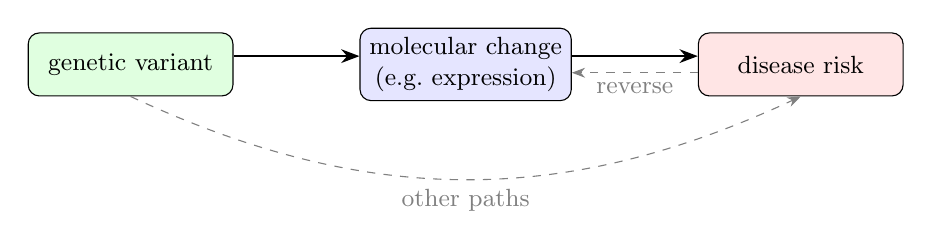
\begin{tikzpicture}[>=Stealth, every node/.style={font=\small}, box/.style={draw, rounded corners, minimum width=2.6cm, minimum height=0.8cm, align=center}]
    \node[box, fill=green!12] (g) {genetic variant};
    \node[box, fill=blue!10, right=1.6cm of g] (m) {molecular change\\(e.g.\ expression)};
    \node[box, fill=red!10, right=1.6cm of m] (d) {disease risk};
    \draw[->, thick] ([yshift=3pt]g.east) -- ([yshift=3pt]m.west);
    \draw[->, thick] ([yshift=3pt]m.east) -- ([yshift=3pt]d.west);
    \draw[->, dashed, gray] ([yshift=-3pt]d.west) -- ([yshift=-3pt]m.east) node[midway, below] {reverse};
    \draw[->, dashed, gray] (g.south) to[out=-25, in=-155] node[midway, below] {other paths} (d.south);
  \end{tikzpicture}
  \caption{Molecular mediators of genetic effects. We would like to find molecular changes on the causal path from a variant to disease. Disease can also change molecular phenotypes (reverse causation), and a variant can affect disease through other paths.}
  \label{fig:mediation}
\end{figure}

%======================================================================
\section{Molecular QTLs}
%======================================================================

\subsection{Layers of omics}

Any molecular readout that can be measured at scale across many individuals can be associated with genotype. The readouts follow the layers of gene regulation met in earlier chapters:
\begin{itemize}
  \item the \emph{genome}: the genetic variants themselves;
  \item the \emph{epigenome}: transcription factor binding (ChIP-seq), DNA methylation (bisulfite sequencing or, more cheaply and at larger scale, methylation arrays), chromatin accessibility (ATAC-seq, DNase-seq) and histone modifications;
  \item the \emph{transcriptome}: gene expression and splicing (RNA-seq);
  \item the \emph{proteome}: protein levels, now measured for a few thousand proteins in tens of thousands of people with affinity-based assays;
  \item the \emph{metabolome}: small molecules in cells or blood.
\end{itemize}
A QTL for each readout gets its own name (Table~\ref{tab:qtl_types}). The most studied are expression QTLs (eQTLs). A gene with at least one significant eQTL is an \emph{eGene}, a variant significantly associated with its expression is an \emph{eVariant}, and the most significant variant for a gene is the \emph{lead} or \emph{top} variant. The terms are awkward but widely used.

\begin{table}[!htbp]
  \centering
  \caption{Types of molecular QTL. Each associates genotype at a variant with a molecular phenotype measured across individuals.}
  \label{tab:qtl_types}
  \small
  \begin{tabular}{p{3.6cm}p{5.6cm}p{3.6cm}}
    \toprule
    QTL & phenotype & typical assay \\
    \midrule
    eQTL (expression) & RNA level of a gene or transcript & RNA-seq \\
    sQTL (splicing) & inclusion ratio of an exon, ratio of isoforms, intron usage & RNA-seq \\
    pQTL (protein) & protein level of a gene & mass spectrometry, affinity assays \\
    meQTL (methylation) & methylation ratio of a CpG site & bisulfite sequencing, arrays \\
    caQTL (chromatin accessibility) & accessibility of a region & ATAC-seq, DNase-seq \\
    hQTL (histone modification) & ChIP-seq peak height of a histone mark & ChIP-seq \\
    \bottomrule
  \end{tabular}
\end{table}

\subsection{Approaches to interpreting GWAS variants}

QTL mapping is one of several ways to interpret a GWAS association~\citep{albert2015}. The simplest is \emph{annotation overlap}: does the variant fall in a gene, a conserved region, or a ChromHMM promoter or enhancer state in a relevant cell type, as in the \textit{FTO} example? A second is \emph{predictive models}, which score how likely a variant is to be functional, either from annotations and conservation or, as in Chapters 2 and 3, from sequence by \emph{in silico} mutagenesis of a deep learning model. A third is \emph{QTL mapping}, the subject of this chapter, which measures the effect of the variant on a molecular phenotype directly in a population. A fourth, \emph{outlier detection}, looks for individuals whose expression is far outside the population distribution and asks whether they carry rare variants; we return to rare variants in the next chapter.

Why not simply predict the effect of each variant from its annotation? For coding variants the consequences are reasonably well understood. A nonsense variant introduces a premature stop codon, a frameshift changes the reading frame, and both usually truncate the protein or trigger nonsense-mediated decay of the RNA. A missense variant changes one amino acid, which may alter the protein's structure or function but not its dosage. For non-coding variants the picture is murkier. Variants in the 5$'$ untranslated region (UTR) can change how efficiently the RNA is translated, variants in the 3$'$ UTR can change its stability, variants near splice sites can change splicing, which can change either the protein sequence or, through decay of a non-productive isoform, the dosage, and variants in promoters and enhancers can change transcription. Most of these variants have no effect at all. Tools exist that label each variant with its possible consequences, but there are few experimentally labelled examples from which to learn which non-coding variants matter. QTL mapping supplies noisy but genome-wide evidence of exactly that.

%======================================================================
\section{Mapping expression QTLs}
%======================================================================

\subsection{Study design}

An eQTL study needs two measurements on the same individuals (Figure~\ref{fig:study_design}). One is genotype, from DNA sequencing or, more cheaply, a genotyping array followed by imputation (Chapter 11). The other is a molecular readout from one or several tissues, most often RNA-seq. RNA-seq gives two kinds of genetic signal. Comparing expression levels across individuals with different genotypes gives eQTLs. Within an individual who is heterozygous at a variant in the transcribed sequence, reads carrying each allele can be counted separately, which gives \emph{allelic expression} (AE), the subject of Section~\ref{sec:ase}.

\begin{figure}[!htbp]
  \centering
  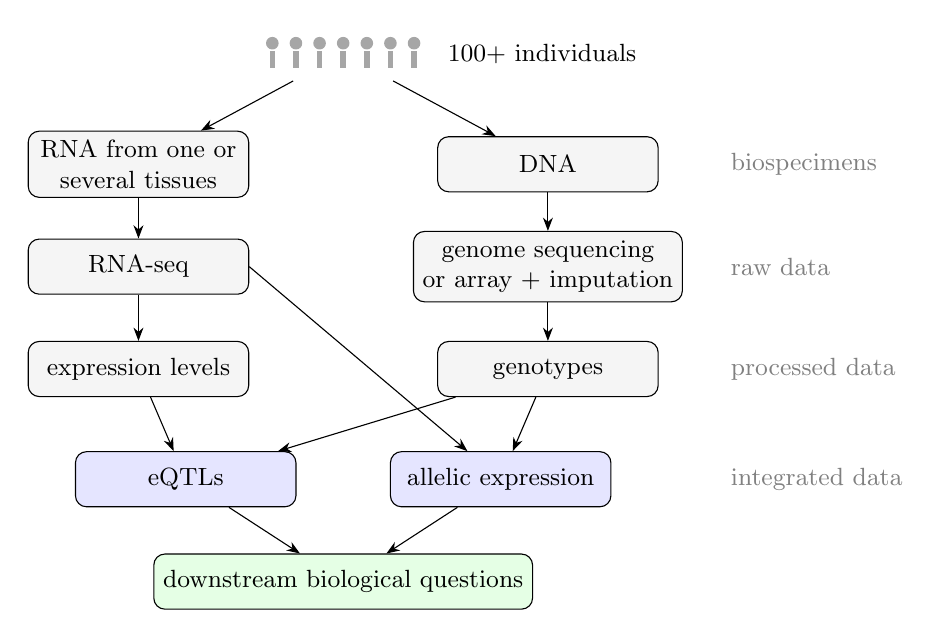
\begin{tikzpicture}[>=Stealth, every node/.style={font=\small}, box/.style={draw, rounded corners, minimum width=2.8cm, minimum height=0.7cm, align=center, fill=gray!8}]
    \node (ppl) at (2.6,0) {\tikz{\foreach \x in {0,0.3,...,2.1} {\fill[gray!70] (\x,0.32) circle (0.08); \draw[gray!70, line width=2pt] (\x,0.22) -- (\x,0);}}};
    \node[right=0.1cm of ppl] {100+ individuals};
    \node[box] (rna) at (0,-1.4) {RNA from one or\\several tissues};
    \node[box] (dna) at (5.2,-1.4) {DNA};
    \node[box] (rseq) at (0,-2.7) {RNA-seq};
    \node[box] (gseq) at (5.2,-2.7) {genome sequencing\\or array + imputation};
    \node[box] (expr) at (0,-4.0) {expression levels};
    \node[box] (geno) at (5.2,-4.0) {genotypes};
    \node[box, fill=blue!10] (eqtl) at (0.6,-5.4) {eQTLs};
    \node[box, fill=blue!10] (ae) at (4.6,-5.4) {allelic expression};
    \node[box, fill=green!10] (down) at (2.6,-6.7) {downstream biological questions};
    \draw[->] (ppl) -- (rna); \draw[->] (ppl) -- (dna);
    \draw[->] (rna) -- (rseq); \draw[->] (dna) -- (gseq);
    \draw[->] (rseq) -- (expr); \draw[->] (gseq) -- (geno);
    \draw[->] (expr) -- (eqtl); \draw[->] (geno) -- (eqtl);
    \draw[->] (rseq.east) -- (ae); \draw[->] (geno) -- (ae);
    \draw[->] (eqtl) -- (down); \draw[->] (ae) -- (down);
    \node[right, gray, align=left] at (7.4,-1.4) {biospecimens};
    \node[right, gray] at (7.4,-2.7) {raw data};
    \node[right, gray] at (7.4,-4.0) {processed data};
    \node[right, gray] at (7.4,-5.4) {integrated data};
  \end{tikzpicture}
  \caption{Design of a molecular QTL study. Genotypes and RNA-seq (or another molecular assay) are measured on the same individuals. Expression levels compared across genotypes give eQTLs; read counts for the two alleles within heterozygous individuals give allelic expression.}
  \label{fig:study_design}
\end{figure}

Sample sizes are modest compared with GWAS. The smallest eQTL studies have around 50 individuals, typical ones a few hundred, well-powered ones around 1000, and meta-analyses tens of thousands. A large GWAS of a disease or of height, by contrast, has hundreds of thousands of individuals. eQTL studies can afford to be smaller because the effects are larger, often a substantial fraction of a gene's expression variance, and, as we discuss next, because they only search a small part of the genome for each gene.

\subsection{The association model}

Let $N$ be the number of individuals and $y_n$ the normalized expression of one gene in individual $n$, for example log counts per million after library size normalization, often followed by an inverse normal transform across individuals. Let $g_n\in\{0,1,2\}$ be the genotype of individual $n$ at one biallelic SNP, coded as the number of copies of the alternative (or minor) allele. Imputed genotypes give an expected count, or \emph{dosage}, in $[0,2]$. The standard model is the linear regression of Chapter 1,
\begin{equation}
  y_n = \mu + \beta g_n + \vx_n^\top\boldsymbol{\delta} + \epsilon_n, \qquad \epsilon_n\sim\Normal(0,\sigma^2),
  \label{eq:eqtl_lm}
\end{equation}
where $\mu$ is the intercept, $\beta$ is the eQTL effect size, $\vx_n\in\R^C$ is a vector of $C$ covariates (sex, genotype principal components for ancestry, technical factors, and the hidden factors of Section~\ref{sec:hidden}) with coefficients $\boldsymbol{\delta}\in\R^C$, and $\sigma^2$ is the noise variance. Coding the genotype as an allele count assumes the two copies of the gene act additively: the heterozygote is halfway between the two homozygotes. This is a reasonable default, since what happens on one chromosome is mostly independent of what happens on the other, and it is the same additive model used for GWAS. We test $H_0:\beta=0$ with the $t$ statistic $\hat\beta/\widehat{\text{se}}(\hat\beta)$, which has a $t$ distribution with $N-2-C$ degrees of freedom under the null. Figure~\ref{fig:eqtl_example} shows a simulated eQTL.

\begin{figure}[!htbp]
  \centering
  \includegraphics[width=0.5\linewidth]{eqtl_example.pdf}
  \caption{A simulated eQTL in $N=300$ individuals: normalized expression of a gene against genotype at a nearby SNP, with the least-squares fit of~\eqref{eq:eqtl_lm} (red). Each copy of allele A raises expression by about half a standard deviation.}
  \label{fig:eqtl_example}
\end{figure}

When individuals are related, or the cohort has strong population structure, the linear mixed models of Chapter 11 replace~\eqref{eq:eqtl_lm}, with a random effect whose covariance is the genetic relatedness matrix. Simple regression remains the most common choice, and fast matrix implementations test all SNP-gene pairs in a study in minutes~\citep{shabalin2012}.

\subsection{Cis windows and the testing burden}

Which SNPs should be tested for each gene? Empirically, by far the strongest genetic effects on a gene's expression come from variants close to it. The usual practice is to test every SNP within a window, typically 1\,Mb on either side of the transcription start site (TSS). These are \emph{cis}-eQTLs. With roughly one common SNP per kilobase, a 2\,Mb window holds of the order of $M=2000$ SNPs, compared with millions for a GWAS. For chromatin phenotypes such as histone marks or accessibility, genetic effects are even more local, and the window is often only the peak itself plus a few kilobases.

The smaller search space is the second reason eQTL studies work at modest sample size. With Bonferroni correction (below), a GWAS needs a p value below $0.05/(3\times10^6)\approx 1.7\times10^{-8}$, while a single gene's cis window needs $0.05/2000=2.5\times10^{-5}$.

\subsection{Multiple testing at two levels}

Multiple testing in an eQTL study has two levels. For each gene we test $M$ SNPs, and we do this for $P$ genes, typically $P\approx 20{,}000$. The usual strategy is first to compute one p value per gene for the null hypothesis that no SNP in its window affects it, and then to control the false discovery rate across genes.

\paragraph{Within a gene.} Let $p_1,\dots,p_M$ be the p values of the SNPs in the window, and $p_{\min}=\min_m p_m$. Under the null each $p_m$ is uniform on $[0,1]$, so for a threshold $t$ the union bound gives
\begin{equation}
  \Pr(p_{\min}\leq t) = \Pr\Big(\bigcup_{m=1}^M\{p_m\leq t\}\Big) \leq \sum_{m=1}^M\Pr(p_m\leq t) = Mt.
\end{equation}
Choosing $t=0.05/M$ controls the probability of any false positive in the window at 5\%; this is the \emph{Bonferroni correction}, and $\min(1,Mp_{\min})$ is the Bonferroni-adjusted gene-level p value. The bound is close to tight when the tests are independent, since then $\Pr(p_{\min}\leq t)=1-(1-t)^M\approx Mt$ for small $t$. SNPs in a cis window are far from independent: LD makes neighbouring SNPs proxies for each other, so the window contains fewer effectively independent tests than $M$, and Bonferroni is conservative.

\emph{Permutation} gives the exact null distribution of $p_{\min}$ for the window. Permuting the expression values across individuals (equivalently, permuting genotype vectors as whole rows, so that LD between SNPs is preserved) breaks any association between genotype and expression while keeping the LD structure and the distribution of expression. For permutations $b=1,\dots,B$ we recompute $p_{\min}^{(b)}$, and the permutation p value is
\begin{equation}
  p_{\text{perm}} = \frac{1+\sum_{b=1}^B\ind\big[p_{\min}^{(b)}\leq p_{\min}\big]}{B+1}.
\end{equation}
Any statistic can be used in place of $p_{\min}$, for example the maximum $|r|$ or $R^2$. Permutation has to recompute the regressions $B$ times for every gene, which is expensive when small gene-level p values must be resolved; FastQTL~\citep{ongen2016} reduces the cost by fitting a beta distribution to a modest number of permuted $p_{\min}$ values and extrapolating. Covariates complicate permutation, because permuting $y$ also breaks its relation to the covariates; the usual remedy is to regress the covariates out of expression first and permute the residuals. Figure~\ref{fig:permutation_null} compares the permutation null of $p_{\min}$ for a window of independent SNPs and for a window with realistic LD. With LD, the 5\% permutation threshold is several times less stringent than Bonferroni, as if the window contained only a quarter of its SNPs.

\begin{figure}[!htbp]
  \centering
  \includegraphics[width=0.85\linewidth]{permutation_null.pdf}
  \caption{Permutation null distribution of the minimum p value across a cis window of $M=330$ SNPs in $N=200$ individuals, from 4000 permutations of a null expression vector. Left, SNPs simulated independently; right, SNPs simulated with block-like LD. The Bonferroni threshold $0.05/M$ (red, dashed) matches the permutation 5\% threshold (blue) for independent SNPs but is conservative with LD. $M_{\text{eff}}=0.05/t_{\text{perm}}$ is the number of independent tests that would give the same threshold.}
  \label{fig:permutation_null}
\end{figure}

\paragraph{Across genes.} Controlling the probability of any false positive across $20{,}000$ genes would be very stringent. Instead we control the \emph{false discovery rate} (FDR), the expected fraction of false positives among the genes we call significant,
\begin{equation}
  \text{FDR} = \E\left[\frac{V}{\max(R,1)}\right],
\end{equation}
where $R$ is the number of genes called eGenes and $V$ the number of those that are null. If we report 5000 eGenes at 10\% FDR, we expect about 500 to be false positives, though we do not know which. The Benjamini-Hochberg (BH) procedure~\citep{benjamini1995} takes the $P$ gene-level p values, sorts them, $p_{(1)}\leq\dots\leq p_{(P)}$, finds the largest $k$ such that
\begin{equation}
  p_{(k)} \leq \frac{k}{P}q,
\end{equation}
and calls the genes with the $k$ smallest p values significant. For independent (or positively dependent) tests this controls the FDR at level $q$. One way to see why: if all $P$ genes were null, about $Pt$ of them would have p values below $t$, so with $k$ genes below $t=p_{(k)}$ the estimated fraction of false discoveries is $Pp_{(k)}/k$, and BH picks the largest set for which this estimate is at most $q$. The $q$-value approach~\citep{storey2003} also estimates the fraction of genes that are null, which gains power when many genes are eGenes. GTEx and most other studies apply the FDR procedure to permutation-based gene-level p values and then, within each eGene, call as eVariants the SNPs whose nominal p values fall below a gene-specific threshold derived from the gene-level cutoff.

%======================================================================
\section{Hidden confounders}
\label{sec:hidden}
%======================================================================

\subsection{Sources of unwanted variation}

Large omics data sets always contain variation that is not the biology we want to study. Some is technical: who prepared the samples, on which day, with which reagent batch, on which sequencing machine. Many eQTL studies use post-mortem tissue, where the \emph{ischaemic time} between death and preservation degrades RNA, and the RNA integrity number (RIN) measures the result. Some is biological but not of interest here: age, sex, environment, recent infections, and in bulk tissue the proportions of different cell types, which vary between people and between pieces of tissue. In GTEx, a study of almost 1000 post-mortem donors and around 50 tissues~\citep{gtex2020}, sample collection variables (ventilator use, ischaemic time, RIN), sequencing batch and library construction are each associated with the main axes of expression variation in many tissues, with $R^2$ up to about 0.3, and estimated cell type proportions are associated to a similar degree.

Such factors affect many genes at once. They do not usually create false eQTLs, because they are not associated with the genotype of a particular SNP, but they add noise to every test and so reduce power. Known factors can be included as covariates in~\eqref{eq:eqtl_lm}. Unknown ones have to be inferred from the expression data.

\subsection{PEER: a factor model for expression}

Chapter 8 introduced factor analysis, $\mY\approx\mX\mW^\top$, and its Bayesian version with an automatic relevance determination (ARD) prior. Because confounders affect many genes, they appear as low-rank structure in the expression matrix, and factor analysis is a natural way to estimate them. PEER (probabilistic estimation of expression residuals)~\citep{stegle2010,stegle2012} combines this with the genetic and known covariate effects in one model (Figure~\ref{fig:peer_model}).

Let $\mY\in\R^{N\times P}$ be the expression matrix of $N$ individuals and $P$ genes (the PEER paper writes the transpose, genes by individuals). The model decomposes it into four parts,
\begin{equation}
  \mY = \underbrace{\mS\mW_S^\top}_{\text{genotype}} + \underbrace{\mF\mW_F^\top}_{\text{known factors}} + \underbrace{\mX\mW^\top}_{\text{hidden factors}} + \mE,
  \label{eq:peer}
\end{equation}
where $\mS\in\{0,1,2\}^{N\times M}$ holds the genotypes of $M$ SNPs with effects $\mW_S\in\R^{P\times M}$; $\mF\in\R^{N\times C}$ holds $C$ measured covariates such as age, sex and batch, with coefficients $\mW_F\in\R^{P\times C}$; $\mX\in\R^{N\times K}$ holds $K$ hidden factors with loadings $\mW\in\R^{P\times K}$; and $\mE\in\R^{N\times P}$ is noise. Element-wise, for gene $p$ and individual $n$,
\begin{equation}
  y_{np}\sim\Normal\Big(\sum_m s_{nm}w^S_{pm}+\sum_c f_{nc}w^F_{pc}+\sum_{k=1}^K x_{nk}w_{pk},\ \tau_p^{-1}\Big),
\end{equation}
with a noise precision $\tau_p$ for each gene, as in factor analysis. The hidden-factor part has the priors of Chapter 8,
\begin{align}
  x_{nk}&\sim\Normal(0,1), & w_{pk}&\sim\Normal(0,\alpha_k^{-1}), & \alpha_k&\sim\Gam(a_\alpha,b_\alpha), & \tau_p&\sim\Gam(a_\tau,b_\tau).
  \label{eq:peer_priors}
\end{align}
The prior precision $\alpha_k$ is shared by all loadings of factor $k$. This is ARD again: if the data do not support factor $k$, $\alpha_k$ grows, the prior variance $1/\alpha_k$ of its loadings shrinks to zero, and the factor is switched off. To see how $\alpha_k$ is set, consider the terms of the log joint density that involve it,
\begin{multline}
  \sum_{p=1}^P\log\Normal(w_{pk}\mid0,\alpha_k^{-1}) + \log\Gam(\alpha_k\mid a_\alpha,b_\alpha) \\ = \frac{P}{2}\log\alpha_k - \frac{\alpha_k}{2}\|\vw_k\|^2 + (a_\alpha-1)\log\alpha_k - b_\alpha\alpha_k + \text{const},
\end{multline}
where $\vw_k\in\R^P$ is column $k$ of $\mW$. Setting the derivative with respect to $\alpha_k$ to zero gives
\begin{equation}
  \hat\alpha_k = \frac{P+2(a_\alpha-1)}{\|\vw_k\|^2+2b_\alpha}\approx\frac{P}{\|\vw_k\|^2},
\end{equation}
the inverse of the mean squared loading. A factor with small loadings gets a large $\alpha_k$, which shrinks its loadings further at the next update, and the iteration drives it to zero. In a variational treatment $\|\vw_k\|^2$ is replaced by its posterior expectation. ARD makes the choice of $K$ less critical: we can set $K$ generously and let the model prune unneeded factors. PEER fits the whole model by mean-field variational Bayes (coordinate ascent variational inference, Chapter 10), which approximates the posterior over $\mX$, $\mW$, $\boldsymbol{\alpha}$ and $\boldsymbol{\tau}$ by a product of independent factors and updates each in turn.

\begin{figure}[!htbp]
  \centering
  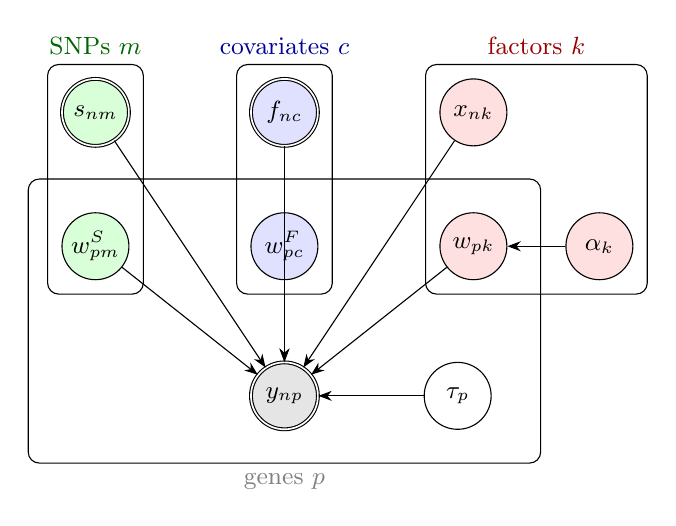
\begin{tikzpicture}[>=Stealth, every node/.style={font=\small},
      lat/.style={circle, draw, minimum size=0.85cm, inner sep=0pt},
      obs/.style={circle, draw, double, minimum size=0.85cm, inner sep=0pt},
      plate/.style={draw, rounded corners, inner sep=5pt}]
    \node[obs, fill=green!15] (s) at (0,2.6) {$s_{nm}$};
    \node[lat, fill=green!15] (ws) at (0,0.9) {$w^S_{pm}$};
    \node[obs, fill=blue!12] (f) at (2.4,2.6) {$f_{nc}$};
    \node[lat, fill=blue!12] (wf) at (2.4,0.9) {$w^F_{pc}$};
    \node[lat, fill=red!12] (x) at (4.8,2.6) {$x_{nk}$};
    \node[lat, fill=red!12] (w) at (4.8,0.9) {$w_{pk}$};
    \node[lat, fill=red!12] (al) at (6.4,0.9) {$\alpha_k$};
    \node[obs, fill=gray!20] (y) at (2.4,-1.0) {$y_{np}$};
    \node[lat] (tau) at (4.6,-1.0) {$\tau_p$};
    \draw[->] (s) -- (y); \draw[->] (ws) -- (y);
    \draw[->] (f) -- (y); \draw[->] (wf) -- (y);
    \draw[->] (x) -- (y); \draw[->] (w) -- (y);
    \draw[->] (al) -- (w); \draw[->] (tau) -- (y);
    \node[plate, fit=(s)(ws), label={[green!40!black]above:SNPs $m$}] {};
    \node[plate, fit=(f)(wf), label={[blue!60!black]above:covariates $c$}] {};
    \node[plate, fit=(x)(w)(al), label={[red!60!black]above:factors $k$}] {};
    \node[plate, fit=(ws)(wf)(w)(y)(tau), inner sep=12pt, label={[gray]below:genes $p$}] {};
  \end{tikzpicture}
  \caption{Graphical model of PEER, after \citet{stegle2010}. Double circles are observed; plates denote replication over SNPs, covariates, hidden factors and genes (the plate over individuals $n$, which contains $s_{nm}$, $f_{nc}$, $x_{nk}$ and $y_{np}$, is omitted for clarity). The ARD precision $\alpha_k$ controls whether hidden factor $k$ is used.}
  \label{fig:peer_model}
\end{figure}

\subsection{PEER in practice}

Fitting all four components of~\eqref{eq:peer} jointly is slow and difficult. In practice the genotype term is left out of the factor model: the known covariates and hidden factors are fitted first, as a pre-processing step, and the eQTL tests are then run with the simple regression~\eqref{eq:eqtl_lm}, either on the residuals or with the inferred factors $\hat\mX$ included as covariates. GTEx chose the number of PEER factors by sample size, using more factors for tissues with more samples. Simpler alternatives work about as well: taking the top principal components of the expression matrix as covariates, as in Chapter 8, matches or outperforms PEER in benchmarks~\citep{zhou2022pca}.

Removing hidden factors greatly increases the number of eQTLs found. In GTEx tissues, the number of eGenes detected at 5\% FDR roughly doubles as the number of PEER factors included as covariates increases from 0 to 60, with diminishing returns beyond that~\citep{fan2020}. Figure~\ref{fig:hidden_factors} shows the same effect on simulated data, which also shows ARD at work. The simulated expression of $P=2000$ genes in $N=200$ individuals has $K=10$ hidden factors and one cis SNP per gene, 30\% of which have a genetic effect. An ARD factor analysis model started with 30 factors keeps exactly 10 (Figure~\ref{fig:hidden_factors}a), and regressing out these factors finds as many eGenes as regressing out the true factors, three times as many as with no correction (Figure~\ref{fig:hidden_factors}b). Regressing out expression principal components improves power up to the true number of factors. Beyond that, extra components capture noise; removing them costs degrees of freedom and removes some genetic signal by chance, so power declines. In real data, with many confounders of decreasing strength, the curve usually rises and then plateaus instead.

\begin{figure}[!htbp]
  \centering
  \begin{subfigure}[b]{0.48\linewidth}
    \includegraphics[width=\linewidth]{ard_factors.pdf}
    \caption{}
  \end{subfigure}\hfill
  \begin{subfigure}[b]{0.48\linewidth}
    \includegraphics[width=\linewidth]{hidden_factors_power.pdf}
    \caption{}
  \end{subfigure}
  \caption{Removing hidden confounders from simulated expression ($N=200$ individuals, $P=2000$ genes, $K=10$ hidden factors). (a) Prior variances $1/\alpha_k$ of the factors of an ARD factor analysis model fitted with 30 factors (the switched-off factors are at the numerical floor $10^{-8}$). (b) eGenes detected at 5\% FDR after regressing out increasing numbers of expression principal components (blue), the 10 active ARD factors (dotted) or the true factors (dashed); the two horizontal lines coincide. The simulation has 617 true eGenes.}
  \label{fig:hidden_factors}
\end{figure}

There are two caveats. First, the factors should capture confounders, not the genetic signal itself. Cis effects are specific to one gene each and are not low-rank, so they survive. A trans-acting variant that changes the expression of many genes, for example through a transcription factor, does produce low-rank structure, and regressing out factors can remove it; hidden-factor correction is therefore risky for trans-eQTL analysis. Second, factors can capture interesting biology, such as cell type composition or an immune response. Removing them helps in finding eQTLs that act in all conditions, at the cost of hiding those whose effect depends on the condition (Section~\ref{sec:interaction}).

%======================================================================
\section{Cis and trans effects}
%======================================================================

A cis-eQTL acts on the copy of the gene on the same chromosome, typically through a promoter or enhancer variant that changes transcription factor binding (Figure~\ref{fig:cis_trans}, top). Cis-eQTLs are the classical eQTL: they are robust, replicate well between studies, and can be found with as few as 70 individuals. A \emph{trans}-eQTL acts at a distance, usually on another chromosome. A typical mechanism is a variant that changes the expression or the protein sequence of a transcription factor, which then changes the expression of the factor's targets throughout the genome (Figure~\ref{fig:cis_trans}, bottom). Trans effects are biologically interesting, since they reveal regulatory networks, but they are hard to find and to replicate. Each effect is small, and without a window to restrict the search we are back to testing millions of SNPs per gene, with a testing burden of millions of SNPs times $20{,}000$ genes. Reliable trans-eQTL mapping needs thousands of individuals, and false positives from technical artefacts, such as reads from one gene mis-mapped to a paralogous gene elsewhere in the genome, are a constant worry.

The cis-trans distinction is about mechanism, not distance alone: a cis effect is one that acts only on the allele on the same DNA molecule. This is what allele-specific expression measures, as we see next. In practice, eQTL studies use physical distance as a proxy and call any SNP within 1\,Mb of a gene cis.

\begin{figure}[!htbp]
  \centering
  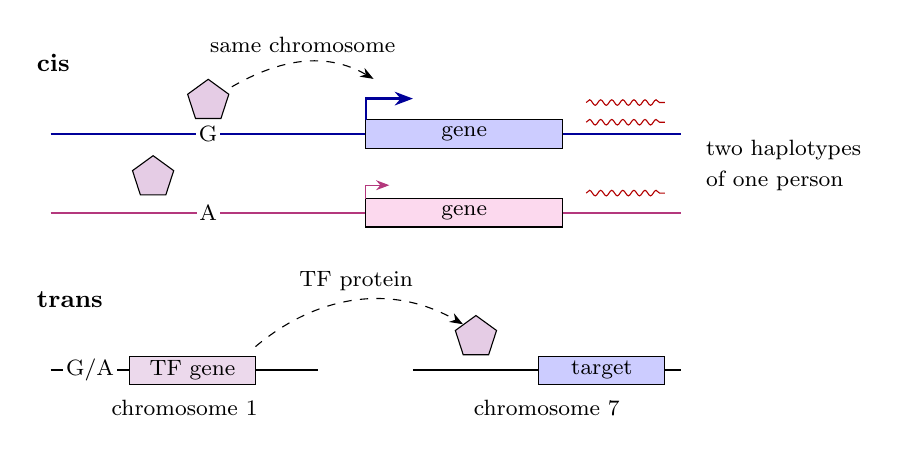
\begin{tikzpicture}[>=Stealth, every node/.style={font=\small}, tf/.style={regular polygon, regular polygon sides=5, draw, fill=violet!20, minimum size=0.55cm, inner sep=0pt}]
    % cis
    \node[anchor=west] at (-0.3,0.9) {\textbf{cis}};
    \draw[thick, blue!60!black] (0,0) -- (8,0);
    \draw[fill=blue!20] (4,-0.18) rectangle (6.5,0.18);
    \node at (5.25,0) {\footnotesize gene};
    \draw[->, thick, blue!60!black] (4,0.18) -- (4,0.45) -- (4.6,0.45);
    \node[tf] at (2,0.42) {};
    \node[fill=white, inner sep=1pt] at (2,0) {\footnotesize G};
    \draw[->, dashed] (2.3,0.6) to[out=30, in=150] node[above] {\footnotesize same chromosome} (4.1,0.7);
    \draw[thick, magenta!70!black] (0,-1.0) -- (8,-1.0);
    \draw[fill=magenta!15] (4,-1.18) rectangle (6.5,-0.82);
    \node at (5.25,-1.0) {\footnotesize gene};
    \draw[->, magenta!70!black] (4,-0.82) -- (4,-0.65) -- (4.3,-0.65);
    \node[fill=white, inner sep=1pt] at (2,-1.0) {\footnotesize A};
    \node[tf] at (1.3,-0.55) {};
    \draw[decorate, decoration={snake, amplitude=1pt, segment length=4pt}, red!70!black] (6.8,0.15) -- (7.8,0.15);
    \draw[decorate, decoration={snake, amplitude=1pt, segment length=4pt}, red!70!black] (6.8,0.40) -- (7.8,0.40);
    \draw[decorate, decoration={snake, amplitude=1pt, segment length=4pt}, red!70!black] (6.8,-0.75) -- (7.8,-0.75);
    \node[right, align=left] at (8.2,-0.4) {\footnotesize two haplotypes\\\footnotesize of one person};
    % trans
    \begin{scope}[yshift=-3.0cm]
      \node[anchor=west] at (-0.3,0.9) {\textbf{trans}};
      \draw[thick] (0,0) -- (3.4,0);
      \draw[fill=violet!15] (1.0,-0.18) rectangle (2.6,0.18);
      \node at (1.8,0) {\footnotesize TF gene};
      \node[fill=white, inner sep=1pt] at (0.5,0) {\footnotesize G/A};
      \node[below] at (1.7,-0.25) {\footnotesize chromosome 1};
      \draw[thick] (4.6,0) -- (8,0);
      \draw[fill=blue!20] (6.2,-0.18) rectangle (7.8,0.18);
      \node at (7.0,0) {\footnotesize target};
      \node[below] at (6.3,-0.25) {\footnotesize chromosome 7};
      \node[tf] (t) at (5.4,0.42) {};
      \draw[->, dashed] (2.6,0.3) to[out=40, in=150] node[above] {\footnotesize TF protein} (t.north west);
    \end{scope}
  \end{tikzpicture}
  \caption{Cis and trans effects. Top: a cis-regulatory variant changes binding of a transcription factor (pentagon) near a gene and so changes expression only of the copy of the gene on the same chromosome, giving more RNA from the G haplotype. Bottom: a trans effect, in which a variant in or near a transcription factor (TF) gene changes the TF's level or activity, which changes expression of its target genes elsewhere in the genome, on both of their copies.}
  \label{fig:cis_trans}
\end{figure}

%======================================================================
\section{Linkage disequilibrium and the causal variant}
%======================================================================

An eQTL association has the same problem as a GWAS association: LD. Figure~\ref{fig:ld_locus} shows a simulated cis window in which one SNP affects expression. Many SNPs in high LD with it are almost as significant, SNPs in moderate LD are moderately significant, and with a little noise the most significant SNP need not be the causal one. SNPs in LD act as proxies, or \emph{tag SNPs}, for the causal variant. The ease of finding an associated locus and the difficulty of finding the variant within it are two sides of the same coin. Fine-mapping methods (Chapter 11), such as SuSiE~\citep{wang2020susie}, compute for each SNP the posterior probability that it is causal and report credible sets that contain a causal variant with high probability, allowing for several causal variants per gene. Functional annotations can sharpen the posterior (Section~\ref{sec:annotations}). The definitive test is experimental: editing the variant with CRISPR and measuring expression, which has been done for the lead variants of some eQTLs.

\begin{figure}[!htbp]
  \centering
  \includegraphics[width=0.7\linewidth]{ld_locus.pdf}
  \caption{A simulated cis-eQTL with one causal SNP (diamond) among 260 SNPs with block-like LD, in $N=500$ individuals. Each point is a SNP, coloured by its LD ($r^2$) with the most significant (lead) SNP. SNPs in high LD with the causal variant are nearly as significant as the causal variant.}
  \label{fig:ld_locus}
\end{figure}

%======================================================================
\section{Allele-specific expression}
\label{sec:ase}
%======================================================================

\subsection{Two views of the same cis effect}

A cis-eQTL can be seen in two ways (Figure~\ref{fig:ase}). Across individuals, those with more copies of the high-expression allele have higher total expression of the gene. Within a single individual who is heterozygous at the regulatory variant, the copy of the gene on the haplotype with the high-expression allele produces more RNA than the copy on the other haplotype. (A \emph{haplotype} is the sequence of one of the two copies of a chromosome, one inherited from each parent.) To see the within-individual difference we need a way to tell the RNA from the two copies apart. If the individual is also heterozygous at a SNP in the transcribed sequence, for example a coding or UTR SNP with alleles T and C, RNA-seq reads that cover it carry one allele or the other, and counting them measures \emph{allele-specific expression} (ASE). An imbalance away from 50:50 indicates a cis-regulatory difference between the two haplotypes.

\begin{figure}[!htbp]
  \centering
  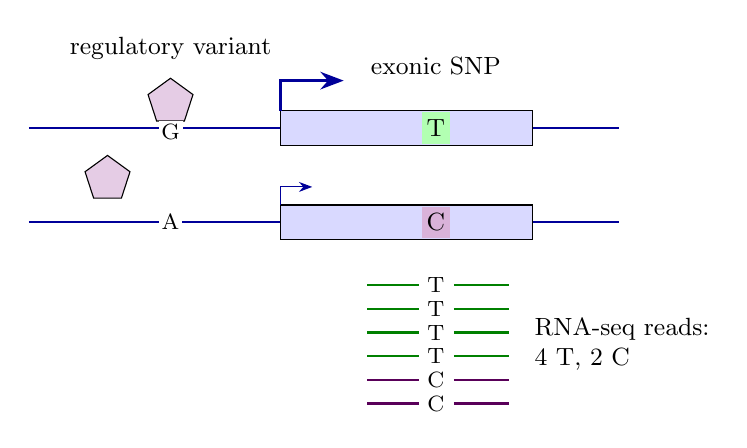
\begin{tikzpicture}[>=Stealth, every node/.style={font=\small}, tf/.style={regular polygon, regular polygon sides=5, draw, fill=violet!20, minimum size=0.6cm, inner sep=0pt}]
    \draw[thick, blue!60!black] (0,0) -- (7.5,0);
    \draw[fill=blue!15] (3.2,-0.22) rectangle (6.4,0.22);
    \fill[green!30] (5.0,-0.2) rectangle (5.35,0.2); \node at (5.17,0) {T};
    \draw[->, very thick, blue!60!black] (3.2,0.22) -- (3.2,0.6) -- (4.0,0.6);
    \node[tf] at (1.8,0.33) {};
    \node[fill=white, inner sep=1pt] at (1.8,-0.05) {\footnotesize G};
    \draw[thick, blue!60!black] (0,-1.2) -- (7.5,-1.2);
    \draw[fill=blue!15] (3.2,-1.42) rectangle (6.4,-0.98);
    \fill[violet!30] (5.0,-1.4) rectangle (5.35,-1.0); \node at (5.17,-1.2) {C};
    \draw[->, blue!60!black] (3.2,-0.98) -- (3.2,-0.75) -- (3.6,-0.75);
    \node[fill=white, inner sep=1pt] at (1.8,-1.2) {\footnotesize A};
    \node[tf] at (1.0,-0.65) {};
    \node[above] at (1.8,0.75) {regulatory variant};
    \node[above] at (5.17,0.55) {exonic SNP};
    % reads
    \foreach \y/\a in {-2.0/T,-2.3/T,-2.6/T,-2.9/T} {
      \draw[green!50!black, thick] (4.3,\y) -- (4.95,\y); \draw[green!50!black, thick] (5.4,\y) -- (6.1,\y);
      \node at (5.17,\y) {\footnotesize \a};}
    \foreach \y/\a in {-3.2/C,-3.5/C} {
      \draw[violet!70!black, thick] (4.3,\y) -- (4.95,\y); \draw[violet!70!black, thick] (5.4,\y) -- (6.1,\y);
      \node at (5.17,\y) {\footnotesize \a};}
    \node[right, align=left] at (6.3,-2.75) {RNA-seq reads:\\4 T, 2 C};
  \end{tikzpicture}
  \caption{Allele-specific expression. In an individual heterozygous at a regulatory variant, a transcription factor (pentagon) binds the G allele but not the A allele, so the copy of the gene on the G haplotype is expressed more. If the individual is also heterozygous at a SNP in the transcript (T/C), RNA-seq reads covering it can be assigned to a haplotype, and the read counts show the imbalance.}
  \label{fig:ase}
\end{figure}

ASE requires an individual to be heterozygous at a transcribed SNP, and, to connect the imbalance to a candidate regulatory variant, the phase of the two SNPs: which allele of the regulatory variant lies on the same haplotype as which allele of the exonic SNP. Phase is estimated statistically from population genotype data or read directly from long reads. The heterozygous exonic SNP is only a marker. It is usually not the cause of the imbalance, which is due to some other variant in cis. The same idea applies to other sequencing assays. In ChIP-seq or ATAC-seq, reads overlapping a heterozygous SNP in a binding site or accessible region measure allele-specific binding or accessibility, and there the SNP being counted is often itself the cause, since a variant inside a binding site can directly change binding.

\subsection{Counting alleles: binomial and beta-binomial models}

Consider one individual and one heterozygous exonic SNP. Let $d$ be the number of reads covering the SNP that carry either allele, $y\leq d$ the number carrying the reference allele, and $\pi$ the expected fraction of reads from the reference haplotype. If reads were independent draws,
\begin{equation}
  y\mid d,\pi \sim \Bin(d,\pi), \qquad \Pr(y\mid d,\pi) = \binom{d}{y}\pi^y(1-\pi)^{d-y},
\end{equation}
and testing for allelic imbalance means testing $H_0:\pi=1/2$. Reads are not independent draws, however. Library preparation amplifies the cDNA by PCR, so several reads can come from one original molecule; mapping and capture efficiencies vary from site to site; and the true imbalance varies between individuals and cells. All of these make the counts more variable than the binomial allows, and a binomial test applied to such data reports far too many significant imbalances.

The \emph{beta-binomial} distribution adds this extra variation by treating $\pi$ as random. Let $\pi\sim\BetaDist(a,b)$ with $a,b>0$ and density
\begin{equation}
  p(\pi\mid a,b) = \frac{\pi^{a-1}(1-\pi)^{b-1}}{\BetaFn(a,b)}, \qquad \BetaFn(a,b)=\int_0^1 u^{a-1}(1-u)^{b-1}du = \frac{\Gamma(a)\Gamma(b)}{\Gamma(a+b)}.
\end{equation}
The beta is the conjugate prior of the binomial (the density has the same form $\pi^{\cdot}(1-\pi)^{\cdot}$ as the likelihood) and is the two-category case of the Dirichlet distribution used for isoform proportions in Chapter 10. Its mean and variance are
\begin{equation}
  \E[\pi] = \frac{a}{a+b}=:\mu, \qquad \Var(\pi) = \frac{ab}{(a+b)^2(a+b+1)} = \frac{\mu(1-\mu)}{c+1},
\end{equation}
where $c=a+b$ is the \emph{concentration}. The ratio of $a$ to $b$ sets the mean, and the concentration sets how tightly $\pi$ is distributed around it. Integrating $\pi$ out gives the beta-binomial,
\begin{align}
  \Pr(y\mid d,a,b) &= \int_0^1\binom{d}{y}\pi^y(1-\pi)^{d-y}\,\frac{\pi^{a-1}(1-\pi)^{b-1}}{\BetaFn(a,b)}\,d\pi \nonumber\\
  &= \binom{d}{y}\frac{1}{\BetaFn(a,b)}\int_0^1\pi^{y+a-1}(1-\pi)^{d-y+b-1}\,d\pi
  = \binom{d}{y}\frac{\BetaFn(y+a,\,d-y+b)}{\BetaFn(a,b)}.
  \label{eq:betabinom}
\end{align}
We write $\BetaBin(y\mid d,\mu,c)$ for this distribution parameterized by its mean fraction $\mu=a/c$ and concentration $c$, so $a=\mu c$ and $b=(1-\mu)c$. The moments follow from the laws of total expectation and variance. The mean is $\E[y]=\E[\E[y\mid\pi]]=d\E[\pi]=d\mu$. For the variance,
\begin{align}
  \Var(y) &= \E[\Var(y\mid\pi)] + \Var(\E[y\mid\pi]) = d\,\E[\pi(1-\pi)] + d^2\Var(\pi) \nonumber\\
  &= d\big(\mu(1-\mu)-\Var(\pi)\big) + d^2\Var(\pi) = d\mu(1-\mu) + d(d-1)\Var(\pi) \nonumber\\
  &= d\mu(1-\mu)\left[1+\frac{d-1}{c+1}\right],
\end{align}
using $\E[\pi(1-\pi)]=\E[\pi]-\E[\pi^2]=\mu-\Var(\pi)-\mu^2$. The first factor is the binomial variance, and the bracket is the overdispersion factor. As $c\to\infty$ it tends to one and the beta-binomial becomes the binomial; small $c$ means noisy allelic counts. Figure~\ref{fig:count_models}a compares a binomial and a beta-binomial with the same mean: the beta-binomial with $c=17$ and $d=30$ has a variance $2.6$ times larger.

\subsection{Counting molecules: Poisson and negative binomial models}

The total read count for a gene in an individual is a count without a fixed number of trials. The basic model is the Poisson, $y\sim\Pois(\lambda)$ with $\Pr(y\mid\lambda)=\lambda^ye^{-\lambda}/y!$, the limit of a binomial with many trials, each with small success probability. Like the binomial it has one parameter: $\E[y]=\Var(y)=\lambda$, so fixing the mean fixes the variance. RNA-seq counts are much more variable between biological replicates than this, for the same reasons as allelic counts and because true expression varies between individuals.

The fix follows the same recipe. Let the rate be random, $\lambda\sim\Gam(\phi,r)$ with shape $\phi$ and rate $r$, density $r^\phi\lambda^{\phi-1}e^{-r\lambda}/\Gamma(\phi)$, mean $\phi/r$ and variance $\phi/r^2$. The gamma is conjugate to the Poisson, and integrating out $\lambda$ gives
\begin{align}
  \Pr(y\mid\phi,r) &= \int_0^\infty \frac{\lambda^ye^{-\lambda}}{y!}\,\frac{r^\phi\lambda^{\phi-1}e^{-r\lambda}}{\Gamma(\phi)}\,d\lambda
  = \frac{r^\phi}{y!\,\Gamma(\phi)}\int_0^\infty\lambda^{y+\phi-1}e^{-(r+1)\lambda}\,d\lambda \nonumber\\
  &= \frac{r^\phi}{y!\,\Gamma(\phi)}\,\frac{\Gamma(y+\phi)}{(r+1)^{y+\phi}}
  = \frac{\Gamma(y+\phi)}{\Gamma(\phi)\,y!}\left(\frac{r}{r+1}\right)^\phi\left(\frac{1}{r+1}\right)^y,
\end{align}
the \emph{negative binomial} distribution, better described as the gamma-Poisson. (Its name comes from another derivation, as the number of failures before the $\phi$-th success in a sequence of coin flips with success probability $r/(r+1)$.) The mean is $m=\E[y]=\E[\lambda]=\phi/r$, and by the law of total variance
\begin{equation}
  \Var(y) = \E[\Var(y\mid\lambda)]+\Var(\E[y\mid\lambda]) = \E[\lambda]+\Var(\lambda) = \frac{\phi}{r}+\frac{\phi}{r^2} = m + \frac{m^2}{\phi}.
\end{equation}
We write $\NB(y\mid m,\phi)$ for the distribution with mean $m$ and shape $\phi$, so $r=\phi/m$. The variance always exceeds the Poisson variance $m$, by an amount controlled by the shape, which plays the role of a concentration: as $\phi\to\infty$ we recover the Poisson. $1/\phi$ is called the dispersion, and the same model underlies standard differential expression tools. Figure~\ref{fig:count_models}b compares a Poisson and a negative binomial with mean 30; with $\phi=8$ the variance is $30+900/8=142.5$ rather than 30.

\begin{figure}[!htbp]
  \centering
  \begin{subfigure}[b]{0.48\linewidth}
    \includegraphics[width=\linewidth]{betabinom.pdf}
    \caption{}
  \end{subfigure}\hfill
  \begin{subfigure}[b]{0.48\linewidth}
    \includegraphics[width=\linewidth]{negbin.pdf}
    \caption{}
  \end{subfigure}
  \caption{Overdispersed count models. (a) Binomial with $d=30$ trials and $\pi=10/17$ and beta-binomial with $d=30$, $a=10$, $b=7$; both have mean 17.6, but the variances are 7.3 and 19.0. (b) Poisson with mean 30 and negative binomial with mean 30 and shape $\phi=8$.}
  \label{fig:count_models}
\end{figure}

\subsection{Combining total and allele-specific counts}

The combined haplotype test (CHT)~\citep{mcvicker2013}, implemented in WASP~\citep{vandegeijn2015}, uses both the between-individual signal in total counts and the within-individual signal in allelic counts to test a candidate cis-regulatory SNP. We describe a simplified version. Let $\theta_R$ and $\theta_A$ be the expression of one copy of the gene on a haplotype carrying the reference and the alternative allele of the test SNP. The expected allelic fraction in a heterozygote is the \emph{allelic imbalance}
\begin{equation}
  \pi = \frac{\theta_R}{\theta_R+\theta_A},
\end{equation}
and the expected total expression of individual $n$ depends on their genotype at the test SNP,
\begin{equation}
  \lambda_n = T_n\times\begin{cases} 2\theta_R & \text{if $n$ is homozygous reference},\\ \theta_R+\theta_A & \text{if $n$ is heterozygous},\\ 2\theta_A & \text{if $n$ is homozygous alternative}, \end{cases}
\end{equation}
where $T_n$ is a scaling factor for how deeply individual $n$ was sequenced. This is the additive model of~\eqref{eq:eqtl_lm} on the count scale. For individual $n$, let $y^t_n$ be the total read count of the gene and $y^a_n$ the number of reads from the haplotype carrying the reference allele of the test SNP, out of $d_n$ reads covering heterozygous exonic SNPs (using the phase to assign reads to haplotypes). The likelihood is
\begin{equation}
  L(\theta_R,\theta_A) = \prod_{n=1}^N \NB\big(y^t_n\mid\lambda_n,\phi\big)\;\prod_{n:\,\text{het}}\BetaBin\big(y^a_n\mid d_n,\pi,c\big)\;\prod_{n:\,\text{hom}}\BetaBin\big(y^a_n\mid d_n,\tfrac12,c\big),
  \label{eq:cht}
\end{equation}
with shape $\phi$ and concentration $c$ estimated across genes. Individuals who are homozygous at the test SNP have the same regulatory allele on both haplotypes, so their allelic counts are expected to be balanced; their term does not depend on $\theta$, but it would show imbalance, and so evidence against this SNP, if the true causal variant were a different one. The test of $H_0:\theta_R=\theta_A$ is a \emph{likelihood ratio test}: maximize~\eqref{eq:cht} with $\theta_R$ and $\theta_A$ free and with $\theta_R=\theta_A$, and compare
\begin{equation}
  \Lambda = 2\left[\log L(\hat\theta_R,\hat\theta_A) - \log L(\hat\theta_0,\hat\theta_0)\right]
\end{equation}
with a $\chi^2_1$ distribution, which by Wilks' theorem is its distribution under the null for large samples. The full CHT also models genotyping errors and estimates the dispersions per individual. WASP also corrects \emph{reference mapping bias}: reads carrying the reference allele align to the reference genome slightly more easily than reads carrying the alternative allele, which mimics allelic imbalance. WASP flips the allele in each read that overlaps a SNP, remaps it, and discards reads that do not map to the same place. RASQUAL~\citep{kumasaka2016} is a related model that combines the two signals and also handles uncertainty in phasing.

\subsection{Calibration and power}

Results of genome-wide tests are summarized by \emph{quantile-quantile (QQ) plots} (Figure~\ref{fig:ase_qq}). If the test is calibrated, its p values are uniform on $[0,1]$ under the null. We sort the $J$ observed p values and plot $-\log_{10}$ of each against $-\log_{10}$ of the corresponding uniform quantile, $(i-0.5)/J$ for the $i$-th smallest. If there is no signal, the points lie on the diagonal. True associations bend the curve upward at the right, while a curve that leaves the diagonal from the start indicates a miscalibrated test or confounding.

Figure~\ref{fig:ase_qq} shows both effects on simulated data with 20 individuals and 2000 SNP-gene pairs, 20\% with a true cis effect, using overdispersed counts ($\phi=10$, $c=30$). On null genes (panel a), a binomial test of allelic imbalance is badly inflated: 14\% of null tests have $p<0.05$. The beta-binomial test with the correct concentration is calibrated (5.4\%). On all genes (panel b), the combined test of~\eqref{eq:cht} finds more than twice as many associations at 5\% FDR as a linear regression on log total counts (232 versus 95 of 407 true effects). \citet{vandegeijn2015} found the same in real data: on H3K27ac ChIP-seq from only 10 lymphoblastoid cell lines, where the linear model found almost nothing, the combined test found many histone QTLs, and it also found substantially more eQTLs in 70 lymphoblastoid cell lines.

\begin{figure}[!htbp]
  \centering
  \includegraphics[width=0.9\linewidth]{ase_qq.pdf}
  \caption{QQ plots of simulated allele-specific tests ($N=20$ individuals, 2000 SNP-gene pairs, 20\% with a cis effect, overdispersed counts). (a) Tests of allelic imbalance among heterozygotes on null genes: the binomial test is inflated, the beta-binomial test is calibrated. (b) eQTL tests on all genes: linear regression of log total counts on genotype, and the combined likelihood ratio test of total (negative binomial) and allelic (beta-binomial) counts. Dashed line, $y=x$.}
  \label{fig:ase_qq}
\end{figure}

Why is the within-individual comparison so powerful? The two haplotypes of an individual are in the same cells, in the same tissue, exposed to the same environment and processed in the same experiment. Comparing them is a built-in control: almost all of the technical and environmental variation that differs between people cancels, leaving the effect of the sequence difference. This gives some insight into regulatory variation even with very small samples, where between-individual eQTL mapping fails. It also separates cis from trans effects, since a trans effect, acting through a diffusible factor, affects both copies of a gene equally. The limitations are that a gene must carry a heterozygous transcribed SNP with enough reads in enough individuals, and that the extra machinery (phasing, mapping bias correction, overdispersion) makes the analysis slower and more involved.

%======================================================================
\section{Lessons from tissue atlases}
%======================================================================

\subsection{eQTLs and sQTLs across tissues}

The Genotype-Tissue Expression (GTEx) project collected RNA-seq from around 50 tissues of almost 1000 post-mortem donors, with whole-genome sequencing of each donor~\citep{gtex2017,gtex2020}. The number of samples per tissue ranges from under 100 to around 700, because some tissues are much harder to collect than others. Figure~\ref{fig:gtex_egenes} shows the fraction of tested genes with a significant cis-eQTL or cis-sQTL in each tissue. Discovery grows steadily with sample size and has not saturated, and eQTLs are easier to detect than sQTLs. Across tissues, 95\% of protein-coding genes have at least one cis-eQTL and 79\% at least one cis-sQTL. With larger samples, conditional analysis (adding the lead variant as a covariate and searching again) finds a second, third or further independent eVariant for an increasing fraction of genes, so the one-causal-variant-per-gene picture is a consequence of limited power rather than biology. Trans-eQTLs were found for only on the order of a hundred genes, consistent with their small effects.

\begin{figure}[!htbp]
  \centering
  \includegraphics[width=0.5\linewidth]{slides/gtex_egenes.pdf}
  \caption{Fraction of tested genes with a cis-eQTL (eGenes, dots) or cis-sQTL (sGenes, stars) at 5\% FDR, against the number of samples, for each GTEx tissue (colours). From the GTEx Consortium~\citep{gtex2020}.}
  \label{fig:gtex_egenes}
\end{figure}

\subsection{Sharing of eQTLs across tissues}

How much of the genetic regulation of expression is shared between tissues? The naive approach maps eQTLs separately in each tissue and counts how often an eQTL significant in one is also significant in another. This confuses the absence of evidence with evidence of absence. Tissues differ in sample size and therefore in power, so an eQTL can be significant in one tissue and not another just because the second has fewer samples. Figure~\ref{fig:sharing_naive} shows this for simulated eQTLs whose true effects are identical in two tissues with 500 and 150 samples: of the eQTLs significant in at least one tissue, 77\% are significant only in the larger one and would be called tissue-specific. Early studies made exactly this mistake and concluded that eQTLs are mostly tissue-specific. The general lesson is that comparing ``significant in condition 1'' with ``significant in condition 2'' is not a test of whether the effect differs; that requires a model of the effects in both conditions together.

\begin{figure}[!htbp]
  \centering
  \includegraphics[width=0.62\linewidth]{sharing_naive.pdf}
  \caption{The ``significant here, not there'' fallacy. Simulated $z$ scores for 3000 eQTLs with the same true effect in two tissues, measured in 500 and 150 individuals. Points are coloured by whether they pass $p<10^{-4}$ in both, one or neither tissue. Most eQTLs significant in the larger tissue are not significant in the smaller one, although none is tissue-specific. Dashed line, the expected ratio $\sqrt{150/500}$ of the $z$ scores.}
  \label{fig:sharing_naive}
\end{figure}

Multivariate adaptive shrinkage (mash)~\citep{urbut2019} models the effects jointly from summary statistics. For SNP-gene pair $j$ and tissue $r=1,\dots,R$, let $b_{jr}$ be the true effect, $\hat b_{jr}$ its estimate (from~\eqref{eq:eqtl_lm} or another test) and $s_{jr}$ the standard error of $\hat b_{jr}$. Collect them into vectors $\vbb_j,\vbhat_j\in\R^R$ and the diagonal matrix $\mS_j=\diag(s_{j1}^2,\dots,s_{jR}^2)$. The likelihood treats the estimates as unbiased and normally distributed,
\begin{equation}
  \vbhat_j\mid\vbb_j \sim \Normal(\vbb_j,\mS_j),
\end{equation}
which can be extended to correlated errors when tissues share donors. The prior on the vector of true effects is a mixture of zero-mean multivariate normals,
\begin{equation}
  \vbb_j \sim \sum_{k=1}^K\sum_{l=1}^L \pi_{kl}\,\Normal(\vzero,\omega_l\mU_k), \qquad \sum_{k,l}\pi_{kl}=1,
  \label{eq:mash_prior}
\end{equation}
where each $\mU_k\in\R^{R\times R}$ is a candidate covariance matrix describing a pattern of sharing across tissues, $\omega_l>0$ is one of $L$ scaling factors on a fixed grid, and $\pi_{kl}\geq0$ are mixture weights. The $\mU_k$ include \emph{canonical} matrices (the identity, for independent effects in each tissue; a matrix of ones, for an identical effect in all tissues; and $R$ matrices with a single non-zero diagonal entry, for an effect in only one tissue) and \emph{data-driven} matrices estimated from the strongest associations, for example by PCA or sparse factor analysis of their $z$ scores. Because the prior and likelihood are Gaussian, $\vbb_j$ can be integrated out within each component,
\begin{equation}
  \vbhat_j \sim \sum_{k,l}\pi_{kl}\,\Normal\big(\vzero,\ \omega_l\mU_k+\mS_j\big),
\end{equation}
and only the weights $\pi_{kl}$ are learned, by maximizing this likelihood over many SNP-gene pairs. The problem is convex in $\pi$ and is solved by EM or convex optimization. With the weights fixed, Bayes' rule gives a posterior for each $\vbb_j$ that is again a mixture of normals. For component $(k,l)$ with prior covariance $\mSigma_{kl}=\omega_l\mU_k$, the posterior covariance and mean are
\begin{equation}
  \mV_{jkl} = \big(\mSigma_{kl}^{-1}+\mS_j^{-1}\big)^{-1}, \qquad \vm_{jkl} = \mV_{jkl}\mS_j^{-1}\vbhat_j,
\end{equation}
and the posterior component weights are $\tilde\pi_{jkl}\propto\pi_{kl}\Normal(\vbhat_j;\vzero,\mSigma_{kl}+\mS_j)$. The posterior means shrink noisy estimates toward the sharing patterns that are common in the data, borrowing strength across tissues. Sharing is then assessed on the posterior effects, for example by asking in which tissues the posterior mean has the same sign as, and is within a factor of two of, the strongest effect, and significance by the \emph{local false sign rate} (lfsr), the posterior probability that the sign of the effect is wrong.

Applied to GTEx, mash estimated that the effects of cis-eQTLs are strongly correlated across tissues (Figure~\ref{fig:mash_heatmap}). The brain regions form a highly correlated block, as do related tissues such as the two skin samples, the arteries and the parts of the gut, while testis, liver, whole blood and lymphoblastoid cells are the most distinct. From an expression genetics point of view the many brain regions sampled by GTEx look much alike; more donors would have given more information than more regions.

\begin{figure}[!htbp]
  \centering
  \includegraphics[width=0.62\linewidth]{slides/mash_tissue_correlation.png}
  \caption{Correlation between tissues of cis-eQTL effects in GTEx, estimated by mash. The colour scale starts at 0.3: all tissue pairs are positively correlated. Reproduced from \citet{urbut2019}.}
  \label{fig:mash_heatmap}
\end{figure}

Counting the number of tissues in which each eQTL is active gives a U-shaped distribution: most eQTLs are either specific to one or a few tissues or active in nearly all of them~\citep{gtex2017}. One explanation is the type of regulatory element. A promoter is used by its gene in every tissue in which the gene is expressed, so a promoter variant can act everywhere, while enhancers are often tissue-specific, so an enhancer variant acts only where its enhancer is active. Tissue-specific eQTLs are often shared between tissues with similar cell types. This suggests that the transcription factors that mediate eQTLs tend to be either constitutive or highly specific. Trans-eQTLs appear more tissue-specific than cis-eQTLs, although their lower power makes this hard to establish.

\subsection{Cell type composition and interaction QTLs}
\label{sec:interaction}

Most eQTL atlases are built from bulk tissue, which mixes many cell types, and the proportions vary between samples. Deconvolution methods, such as CIBERSORT (Chapter 8) or the enrichment scores of xCell~\citep{aran2017}, estimate the abundance of each cell type from expression. In GTEx they recover the expected patterns, such as hepatocytes in liver, keratinocytes in skin, myocytes in skeletal muscle, neurons in brain and neutrophils in blood, spleen and lung, and the similarity of tissues in cell type composition correlates with their similarity in eQTL and sQTL sharing~\citep{kimhellmuth2020}. Cell type composition is a major driver of variation in bulk expression between individuals.

If an eQTL acts in only one cell type, its effect in bulk tissue scales with that cell type's proportion. An \emph{interaction QTL} test looks for this,
\begin{equation}
  y_n = \mu + \beta_g g_n + \beta_c c_n + \beta_{gc}\,g_n c_n + \epsilon_n,
  \label{eq:ieqtl}
\end{equation}
where $c_n$ is the estimated proportion (or enrichment score) of the cell type in sample $n$, $\beta_c$ its effect on expression, and $\beta_{gc}$ the interaction: how much the genetic effect changes per unit change in cell type proportion. Testing $\beta_{gc}=0$ identifies cell type interacting eQTLs, many of which turn out to be cell type-specific eQTLs~\citep{kimhellmuth2020}. The test has limited power, because it depends on variation in proportions between samples and on noisy proportion estimates. Single-cell eQTL studies measure cell type-specific effects directly but are so far smaller and cover few tissues. The same interaction model applies to any measured context, such as age, sex, or a stimulus, which we meet again in Section~\ref{sec:coloc}.

%======================================================================
\section{Which variants are causal? Genomic annotations}
\label{sec:annotations}
%======================================================================

Fine-mapping one gene at a time is limited by LD. Pooling information across all genes can help, because the properties that make a variant more likely to be causal, such as lying in accessible chromatin or near the TSS, are shared. \citet{gaffney2012} built a hierarchical model that learns these properties from eQTL data and uses them as a prior for fine-mapping.

For gene $p$ with $M_p$ SNPs in its cis window, let $z_p\in\{0,1,\dots,M_p\}$ indicate the causal SNP, with $z_p=0$ if the gene has no eQTL; the model assumes at most one causal SNP per gene. Let $\va_{pm}\in\R^A$ be a vector of $A$ annotations of SNP $m$, such as indicators for overlapping a DNase I hypersensitive site, a histone mark peak or a predicted transcription factor binding site, and bins of distance to the TSS. The prior is
\begin{equation}
  \Pr(z_p\neq0) = \Pi, \qquad \Pr(z_p=m\mid z_p\neq0) = q_{pm} = \frac{\exp(\vlambda^\top\va_{pm})}{\sum_{m'=1}^{M_p}\exp(\vlambda^\top\va_{pm'})},
\end{equation}
a softmax over the SNPs in the window with annotation weights $\vlambda\in\R^A$, as in the multiclass logistic regression of Chapter 1. Holding the other annotations fixed, a SNP with annotation $a$ is $e^{\lambda_a}$ times more likely to be causal than one without, so $e^{\lambda_a}$ is the enrichment of the annotation. The data enter through the Bayes factor $\text{BF}_{pm}=p(\vy_p\mid z_p=m)/p(\vy_p\mid z_p=0)$ comparing the model in which SNP $m$ affects the expression $\vy_p\in\R^N$ of gene $p$ with the null model, computed from a single-SNP Bayesian regression. The marginal likelihood of gene $p$, relative to the null, is
\begin{equation}
  \frac{p(\vy_p\mid\Pi,\vlambda)}{p(\vy_p\mid z_p=0)} = (1-\Pi) + \Pi\sum_{m=1}^{M_p}q_{pm}\text{BF}_{pm},
\end{equation}
and the posterior probability that SNP $m$ is causal is
\begin{equation}
  r_{pm} = \Pr(z_p=m\mid\vy_p) = \frac{\Pi\,q_{pm}\text{BF}_{pm}}{(1-\Pi)+\Pi\sum_{m'}q_{pm'}\text{BF}_{pm'}}.
\end{equation}
$\Pi$ and $\vlambda$ are estimated by maximizing the product of the marginal likelihoods over all genes with EM. The E-step computes $r_{pm}$. The M-step sets $\Pi$ to the average of $\sum_m r_{pm}$ over genes and fits $\vlambda$ by maximizing $\sum_p\sum_m r_{pm}\log q_{pm}(\vlambda)$, a multiclass logistic regression in which each gene is one example, the classes are its SNPs and the labels are the soft posteriors $r_{pm}$ rather than observed causal variants. We never observe which variant is causal; the model learns from the noisy evidence summarized by the Bayes factors. The same structure is used for GWAS fine-mapping with annotations in Chapter 11.

Figure~\ref{fig:gaffney} shows the results for lymphoblastoid cell lines. SNPs in DNase I hypersensitive sites, which mark accessible chromatin, are about four times as likely to be causal as other SNPs, SNPs in H3K27ac and other active histone mark peaks are also enriched, and SNPs in regions marked by the repressive H3K27me3 are depleted. The enrichments hold for SNPs more than 5\,kb upstream of the TSS, which excludes promoters. The prior probability that a SNP is causal is highest at the TSS and falls quickly with distance, by an order of magnitude within a few tens of kilobases, and at every distance it is higher inside DNase sites. This is why a 1\,Mb window is generous for most eQTLs. Among transcription factors, SNPs in ChIP-seq peaks of factors such as JunD and NF-$\kappa$B are strongly enriched.

\begin{figure}[!htbp]
  \centering
  \includegraphics[width=\linewidth]{slides/gaffney_annotation_enrichment.png}
  \caption{Annotations of causal eQTL variants in lymphoblastoid cell lines. (a) Enrichment ($\log_2$, with 95\% intervals) of causal variants in DNase I hypersensitive sites and histone mark peaks, for all SNPs and (b) for SNPs more than 5\,kb upstream of the TSS. (c) Prior probability that a SNP is the causal variant as a function of position relative to the TSS, for SNPs in DNase sites and active histone marks (blue), in DNase sites (red), on average (grey) and outside DNase sites (green). Reproduced from \citet{gaffney2012}.}
  \label{fig:gaffney}
\end{figure}

Several related models exist. LirNet~\citep{lee2009lirnet} learns, across genes, how a SNP's regulatory features set the strength of its regularization in a sparse regression of expression on genotype. TORUS~\citep{wen2016} extends the hierarchical model to allow several causal SNPs per gene and controls a Bayesian FDR for eGene discovery. SuSiE~\citep{wang2020susie}, the sum of single effects model of Chapter 11, is now the most widely used fine-mapping method; it allows several causal variants, is fitted by coordinate ascent variational inference, and can take annotation-based priors such as those learned by TORUS.

Could sequence-based deep learning models (Chapters 2 and 3) replace this? Models such as Enformer predict the effects of a sequence on chromatin and expression, and so in principle predict the effect of every variant. They are good at predicting local features such as transcription factor binding and accessibility, and expression differences between genes, but not yet at predicting expression differences between individuals from their genotypes. \citet{sasse2023} compared predictions from personal genome sequences with measured brain expression: for most genes the correlation across individuals was near zero, and among genes with significant correlations, about a third had the wrong sign. The models often predict correctly that a variant matters but get the direction of its effect wrong.

%======================================================================
\section{Explaining GWAS associations with QTLs: colocalization}
\label{sec:coloc}
%======================================================================

A GWAS locus and an eQTL for a nearby gene overlap. Does that mean the gene mediates the disease association? Three questions need answers. Is there a significant eQTL in the locus at all? If so, are the GWAS and eQTL association patterns so similar that they probably share a causal variant, or could two different causal variants in LD produce overlapping signals by coincidence? And is the eQTL measured in the right tissue, cell type or cell state? \emph{Colocalization} analysis addresses the second question.

\subsection{The coloc model}

The coloc method~\citep{giambartolomei2014} considers a region of $M$ SNPs and two traits, say the expression of a gene (trait 1) and a disease (trait 2), measured in different samples. It assumes that each trait has at most one causal variant in the region, and compares five hypotheses (Figure~\ref{fig:coloc}):
\begin{itemize}
  \item $H_0$: no association with either trait;
  \item $H_1$: association with trait 1 only;
  \item $H_2$: association with trait 2 only;
  \item $H_3$: association with both traits, with two different causal variants;
  \item $H_4$: association with both traits, with one shared causal variant.
\end{itemize}
$H_4$ is what we hope to find. It does not prove that the gene causes the disease, since the shared variant could affect the disease through another gene, but it is a necessary condition. $H_3$ is the case a naive overlap analysis gets wrong.

Each hypothesis is a set of \emph{configurations}, which say which SNP, if any, is causal for each trait: one configuration for $H_0$, $M$ each for $H_1$, $H_2$ and $H_4$, and $M(M-1)$ for $H_3$. Each configuration gets a prior probability: $p_1$ for a configuration with a causal SNP for trait 1 only, $p_2$ for trait 2 only, $p_1p_2$ for two different causal SNPs, and $p_{12}$ for one shared SNP, with typical defaults $p_1=p_2=10^{-4}$ and $p_{12}=10^{-5}$. Because the two traits are measured in different samples, the likelihood factorizes over traits, and the Bayes factor of a configuration against $H_0$ is the product of a Bayes factor for each trait. Let $\text{BF}^{(1)}_m$ and $\text{BF}^{(2)}_m$ be the Bayes factors for SNP $m$ being the causal variant for traits 1 and 2. Summing over configurations, the posterior probabilities are proportional to
\begin{align}
  \Pr(H_0\mid D) &\propto 1, &
  \Pr(H_1\mid D) &\propto p_1\sum_m \text{BF}^{(1)}_m, \nonumber\\
  \Pr(H_2\mid D) &\propto p_2\sum_m \text{BF}^{(2)}_m, &
  \Pr(H_3\mid D) &\propto p_1p_2\sum_{m\neq m'}\text{BF}^{(1)}_m\text{BF}^{(2)}_{m'}, \nonumber\\
  \Pr(H_4\mid D) &\propto p_{12}\sum_m\text{BF}^{(1)}_m\text{BF}^{(2)}_m,
\end{align}
where $D$ denotes the data for both traits. The $H_3$ sum is computed as $\big(\sum_m\text{BF}^{(1)}_m\big)\big(\sum_{m'}\text{BF}^{(2)}_{m'}\big)-\sum_m\text{BF}^{(1)}_m\text{BF}^{(2)}_m$. $H_4$ wins when both traits put their Bayes factor mass on the same SNPs, and $H_3$ wins when they put it on different SNPs.

The Bayes factors need only summary statistics. Let $\hat\beta_m$ be the estimated effect of SNP $m$ on a trait, with sampling variance $V_m=\text{se}(\hat\beta_m)^2$, so $\hat\beta_m\mid\beta_m\sim\Normal(\beta_m,V_m)$. Under the null $\beta_m=0$, and under the alternative $\beta_m\sim\Normal(0,W)$ with prior variance $W$, so marginally $\hat\beta_m\sim\Normal(0,V_m+W)$. The ratio of the two densities is Wakefield's approximate Bayes factor~\citep{wakefield2009},
\begin{equation}
  \text{BF}_m = \frac{\Normal(\hat\beta_m;0,V_m+W)}{\Normal(\hat\beta_m;0,V_m)} = \sqrt{\frac{V_m}{V_m+W}}\exp\left(\frac{z_m^2}{2}\,\frac{W}{V_m+W}\right),
  \label{eq:abf-12}
\end{equation}
where $z_m=\hat\beta_m/\sqrt{V_m}$. It increases with $z_m^2$, and the prefactor penalizes the alternative for spreading its prior over effects that the data could have shown but did not. Under the single-causal-variant assumption, the Bayes factor of the configuration ``SNP $m$ is causal'' is $\text{BF}_m$ computed from the marginal statistics of SNP $m$ alone, so no LD matrix is needed. The assumption is restrictive when a locus has several causal variants; extensions combine coloc with SuSiE fine-mapping to test each pair of credible sets.

Figure~\ref{fig:coloc} shows coloc on simulated data, with an eQTL study of 500 individuals and a GWAS of 5000. When the same SNP is causal for both traits, the association patterns match and the posterior probability of $H_4$ is 0.99. When the GWAS causal variant is a different SNP in weak LD ($r^2=0.31$) with the eQTL causal variant, both traits show associations across the same region, but their peaks are at different SNPs, and the posterior probability of $H_3$ is 0.94.

\begin{figure}[!htbp]
  \centering
  \includegraphics[width=0.9\linewidth]{coloc_example.pdf}
  \caption{Colocalization on simulated data. Association $-\log_{10}p$ along a region of 200 SNPs for an eQTL ($N=500$, red) and a GWAS ($N=5000$, blue); diamonds mark the causal variants. Left, one shared causal variant; right, distinct causal variants in weak LD. Panel titles give the coloc posterior probabilities of $H_3$ and $H_4$ with default priors and $W=0.15^2$.}
  \label{fig:coloc}
\end{figure}

\subsection{What colocalization has found}

The GTEx consortium ran colocalization for GWAS of many traits, including lipid levels, BMI and autoimmune diseases~\citep{gtex2017}. A substantial fraction of GWAS loci colocalize with an eQTL in at least one tissue, and the colocalizing gene is often not the gene nearest to the lead GWAS variant, as for \textit{FTO}, \textit{IRX3} and \textit{IRX5}. Many loci, however, do not colocalize with any eQTL. Some of this gap is power, but some is because eQTL studies measure the wrong context. Expression effects relevant to an immune disease may only appear when immune cells respond to a challenge, while blood samples contain mostly resting cells. \citet{kimhellmuth2017} stimulated monocytes from 134 donors with bacterial and viral ligands and found eQTLs that appeared only after stimulation, some of which colocalized with autoimmune disease associations that resting-cell eQTLs did not explain. The cell state can matter, not just the cell type.

Why does this matter? Drug targets with human genetic support are more likely to succeed in clinical trials (Chapter 1). The effects involved are small: a typical eQTL changes expression by perhaps 5--10\%, and each GWAS variant changes disease risk slightly, so these results are of little use for predicting who will get a disease. They do give a view of the causal biology of disease in humans, without the limitations of animal models and without a clinical trial.

%======================================================================
\section{Transcriptome-wide association studies}
%======================================================================

A transcriptome-wide association study (TWAS)~\citep{gamazon2015,gusev2016} links expression to a trait through genetically predicted expression (Figure~\ref{fig:twas}). In a \emph{reference panel} with genotypes and expression, we train a model to predict each gene's expression from the genotypes of its cis SNPs,
\begin{equation}
  e_n = \vx_n^\top\vw + \epsilon_n,
\end{equation}
where $e_n$ is the expression of the gene in individual $n$ of the panel, $\vx_n\in\R^M$ holds the standardized genotypes of the $M$ cis SNPs and $\vw\in\R^M$ the weights, usually fitted with the elastic net or lasso of Chapter 1, or with a Bayesian sparse regression. In a GWAS cohort, which has genotypes and the trait but no expression, we then impute expression, $\hat e_n=\vx_n^\top\hat\vw$, and test the association between $\hat e_n$ and the trait.

\begin{figure}[!htbp]
  \centering
  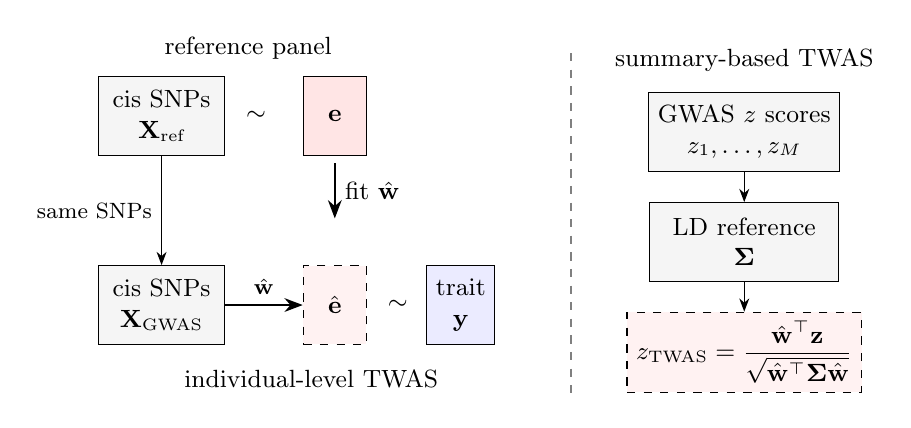
\begin{tikzpicture}[>=Stealth, every node/.style={font=\small},
      mat/.style={draw, minimum width=1.6cm, minimum height=1.0cm, align=center, fill=gray!8}]
    \node[mat] (gref) at (0,0) {cis SNPs\\$\mX_{\text{ref}}$};
    \node[mat, fill=red!10, minimum width=0.8cm] (eref) at (2.2,0) {$\ve$};
    \node at (1.2,0) {$\sim$};
    \node[above] at (1.1,0.6) {reference panel};
    \draw[->, thick] (2.2,-0.6) -- (2.2,-1.3) node[midway, right] {fit $\hat\vw$};
    \node[mat] (ggw) at (0,-2.4) {cis SNPs\\$\mX_{\text{GWAS}}$};
    \node[mat, fill=red!5, minimum width=0.8cm, dashed] (ehat) at (2.2,-2.4) {$\hat\ve$};
    \node[mat, fill=blue!8, minimum width=0.8cm] (trait) at (3.8,-2.4) {trait\\$\vy$};
    \draw[->] (gref.south) -- (ggw.north) node[midway, left] {\footnotesize same SNPs};
    \draw[->, thick] (ggw) -- (ehat) node[midway, above] {\footnotesize$\hat\vw$};
    \node at (3.0,-2.4) {$\sim$};
    \node[below, align=center] at (1.9,-3.1) {individual-level TWAS};
    % summary based
    \node[mat, minimum width=2.4cm] (z) at (7.4,-0.2) {GWAS $z$ scores\\$z_1,\dots,z_M$};
    \node[mat, minimum width=2.4cm] (ld) at (7.4,-1.6) {LD reference\\$\mSigma$};
    \node[mat, fill=red!5, dashed, minimum width=2.6cm] (zt) at (7.4,-3.0) {$z_{\text{TWAS}}=\dfrac{\hat\vw^\top\vz}{\sqrt{\hat\vw^\top\mSigma\hat\vw}}$};
    \draw[->] (z) -- (ld); \draw[->] (ld) -- (zt);
    \node[above] at (7.4,0.45) {summary-based TWAS};
    \draw[dashed, gray] (5.2,0.8) -- (5.2,-3.6);
  \end{tikzpicture}
  \caption{Transcriptome-wide association study. Left: weights $\hat\vw$ predicting a gene's expression from cis SNPs are learned in a reference panel, used to impute expression in a GWAS cohort, and imputed expression is tested for association with the trait. Right: the same test computed from GWAS summary statistics and an LD reference. After \citet{gusev2016}.}
  \label{fig:twas}
\end{figure}

Individual-level GWAS data are often unavailable, but the test can be computed from GWAS summary statistics~\citep{gusev2016}. Let $\mX\in\R^{N\times M}$ be the standardized cis genotypes of the $N$ GWAS individuals and $\vy\in\R^N$ the standardized trait. The marginal $z$ score of SNP $m$ is approximately $z_m=\vx_m^\top\vy/\sqrt N$, where $\vx_m$ is column $m$ of $\mX$, so $\vz=\mX^\top\vy/\sqrt N$. The imputed expression is $\hat\ve=\mX\hat\vw$, with sample variance $\hat\vw^\top\mSigma\hat\vw$, where $\mSigma=\mX^\top\mX/N$ is the LD (correlation) matrix of the SNPs. The $z$ score for the association of $\hat\ve$ with $\vy$ is
\begin{equation}
  z_{\text{TWAS}} = \frac{\hat\ve^\top\vy}{\sqrt N\sqrt{\hat\vw^\top\mSigma\hat\vw}} = \frac{\hat\vw^\top\mX^\top\vy/\sqrt N}{\sqrt{\hat\vw^\top\mSigma\hat\vw}} = \frac{\hat\vw^\top\vz}{\sqrt{\hat\vw^\top\mSigma\hat\vw}},
  \label{eq:twas}
\end{equation}
a weighted sum of the GWAS $z$ scores, normalized by its null standard deviation: under the null $\vz\sim\Normal(\vzero,\mSigma)$, so $\Var(\hat\vw^\top\vz)=\hat\vw^\top\mSigma\hat\vw$. The LD matrix comes from a reference sample of the same ancestry.

TWAS has two attractions. It is signed: the sign of $z_{\text{TWAS}}$ says whether higher genetically predicted expression increases or decreases risk, which is what we need to know to design a drug that inhibits or activates a target. And it is protected against reverse causation. Expression measured in patients reflects the disease as well as causing it; in Alzheimer's disease, for example, microglia in the brain respond to the damage, so much of the expression difference between cases and controls is a consequence of the disease. Genetically predicted expression is fixed at conception and cannot be changed by the disease.

Figure~\ref{fig:twas_pd} shows a TWAS of Parkinson's disease~\citep{li2018leafcutter}, using 537 dorsolateral prefrontal cortex RNA-seq samples from the CommonMind consortium~\citep{fromer2016} as the reference panel and a GWAS of about 14{,}000 cases and 95{,}000 controls~\citep{nalls2014}. With predicted splicing (intron usage quantified by LeafCutter, Chapter 10) as well as predicted expression, 26 genes were associated through splicing and 18 through expression at 5\% FDR. The strongest signal was splicing of \textit{MAPT}, which encodes tau.

\begin{figure}[!htbp]
  \centering
  \includegraphics[width=0.85\linewidth]{slides/twas_parkinsons.png}
  \caption{TWAS of Parkinson's disease using brain expression (blue) and splicing (green) reference panels; dark points are associations shared with monocytes. Each point is a gene's TWAS $z$ score along the genome; dashed lines mark significance at 5\% FDR. Reproduced from \citet{li2018leafcutter}.}
  \label{fig:twas_pd}
\end{figure}

TWAS inherits the limitations of its components. Genes in the same locus have correlated predicted expression, because they share cis SNPs and LD, so a TWAS association, like an overlapping eQTL, can be driven by a neighbouring gene or by a variant acting through another mechanism. TWAS assumes the variants in the predictor affect the trait only through the gene's expression. This is the central assumption of Mendelian randomization, to which TWAS is closely related.

%======================================================================
\section{Mendelian randomization}
%======================================================================

\subsection{Instrumental variables}

Mendelian randomization (MR)~\citep{daveysmith2003} estimates the causal effect of an \emph{exposure} $X$, such as the expression of a gene or a biomarker like LDL cholesterol, on an \emph{outcome} $Y$, such as disease risk. The problem is the usual one of observational data: an association between $X$ and $Y$ can be due to a confounder $U$ that affects both, or to reverse causation. MR uses a genetic variant $G_j$ associated with the exposure as an \emph{instrumental variable} (Figure~\ref{fig:mr_dag}). Alleles are assigned at random at conception, given the parents' genotypes, much as treatments are in a randomized trial, hence the name. The instrument is valid under three assumptions:
\begin{enumerate}
  \item \emph{relevance}: $G_j$ is associated with $X$;
  \item \emph{independence}: $G_j$ is not associated with any confounder $U$ of $X$ and $Y$;
  \item \emph{exclusion restriction}: $G_j$ affects $Y$ only through $X$, with no direct (pleiotropic) path.
\end{enumerate}
In an eQTL setting, the exposure is the expression of a gene and the instrument is a cis-eQTL, which makes the first assumption easy to check and the third plausible but not guaranteed.

\begin{figure}[!htbp]
  \centering
  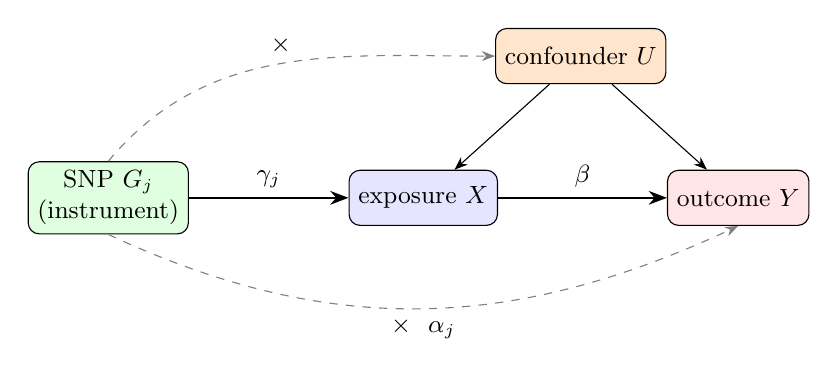
\begin{tikzpicture}[>=Stealth, every node/.style={font=\small}, var/.style={draw, rounded corners, minimum width=1.5cm, minimum height=0.7cm, align=center}]
    \node[var, fill=green!12] (g) at (0,0) {SNP $G_j$\\(instrument)};
    \node[var, fill=blue!10] (x) at (4,0) {exposure $X$};
    \node[var, fill=red!10] (y) at (8,0) {outcome $Y$};
    \node[var, fill=orange!20] (u) at (6,1.8) {confounder $U$};
    \draw[->, thick] (g) -- node[above] {$\gamma_j$} (x);
    \draw[->, thick] (x) -- node[above] {$\beta$} (y);
    \draw[->] (u) -- (x); \draw[->] (u) -- (y);
    \draw[->, dashed, gray] (g.north) to[out=50, in=180] node[midway, above, black] {$\times$} (u.west);
    \draw[->, dashed, gray] (g.south) to[out=-25, in=-155] node[midway, below, black] {$\times$ \ $\alpha_j$} (y.south);
  \end{tikzpicture}
  \caption{Mendelian randomization. A SNP $G_j$ affects the exposure $X$ with effect $\gamma_j$, and $X$ affects the outcome $Y$ with causal effect $\beta$. The SNP must not be associated with the confounder $U$, and must have no direct effect $\alpha_j$ on the outcome (crossed dashed paths).}
  \label{fig:mr_dag}
\end{figure}

\subsection{The ratio estimate}

Write a linear model for the exposure and the outcome,
\begin{equation}
  X = \gamma_jG_j + U + \epsilon_X, \qquad Y = \beta X + \alpha_jG_j + \kappa U + \epsilon_Y,
\end{equation}
where $\gamma_j$ is the effect of SNP $j$ on the exposure, $\beta$ the causal effect of the exposure on the outcome, $\alpha_j$ a direct (pleiotropic) effect of the SNP on the outcome, $\kappa$ the effect of the confounder, and $\epsilon_X,\epsilon_Y$ independent noise. Under the independence assumption $\Cov(G_j,U)=0$, so
\begin{align}
  \Cov(G_j,X) &= \gamma_j\Var(G_j), \\
  \Cov(G_j,Y) &= \beta\Cov(G_j,X) + \alpha_j\Var(G_j) = (\beta\gamma_j+\alpha_j)\Var(G_j).
\end{align}
The regression coefficients of the exposure and the outcome on the SNP are therefore $\gamma_j$ and $\Gamma_j=\beta\gamma_j+\alpha_j$, and these are exactly what GWAS of the exposure and of the outcome estimate. The confounder has dropped out. If the exclusion restriction holds, $\alpha_j=0$ and the \emph{ratio} (Wald) estimate
\begin{equation}
  \hat\beta_j = \frac{\hat\Gamma_j}{\hat\gamma_j} = \frac{\hat\beta_{\text{SNP}\to\text{outcome}}}{\hat\beta_{\text{SNP}\to\text{exposure}}}
\end{equation}
is a consistent estimate of $\beta$. With pleiotropy it estimates $\beta+\alpha_j/\gamma_j$, biased by an amount that is larger for weaker instruments.

\subsection{Multiple instruments}

With $J$ independent instruments (SNPs not in LD with each other), the inverse-variance weighted (IVW) estimate~\citep{burgess2013} combines the ratio estimates. Treating $\hat\gamma_j$ as known and $\text{se}(\hat\beta_j)\approx\text{se}(\hat\Gamma_j)/|\hat\gamma_j|$, weighting each ratio by its inverse variance gives
\begin{equation}
  \hat\beta_{\text{IVW}} = \frac{\sum_j \hat\beta_j\,\hat\gamma_j^2\sigma_j^{-2}}{\sum_j\hat\gamma_j^2\sigma_j^{-2}} = \frac{\sum_j\hat\gamma_j\hat\Gamma_j\sigma_j^{-2}}{\sum_j\hat\gamma_j^2\sigma_j^{-2}},
\end{equation}
where $\sigma_j=\text{se}(\hat\Gamma_j)$. This is the weighted least-squares slope of a regression of $\hat\Gamma_j$ on $\hat\gamma_j$ through the origin. If the pleiotropic effects $\alpha_j$ average to zero (balanced pleiotropy), IVW is still consistent. If they do not (directional pleiotropy, mean $\mu_\alpha\neq0$), IVW is biased.

MR-Egger regression~\citep{bowden2015} relaxes the assumption. Writing $\alpha_j=\mu_\alpha+(\alpha_j-\mu_\alpha)$,
\begin{equation}
  \Gamma_j = \mu_\alpha + \beta\gamma_j + (\alpha_j-\mu_\alpha).
\end{equation}
If the pleiotropic effects are independent of the instrument strengths $\gamma_j$ across SNPs (the InSIDE assumption, instrument strength independent of direct effect), the last term is uncorrelated with $\gamma_j$, and a weighted regression of $\hat\Gamma_j$ on $\hat\gamma_j$ \emph{with an intercept} estimates the causal effect $\beta$ as its slope and the average pleiotropy $\mu_\alpha$ as its intercept. Before fitting, each SNP is oriented so that $\hat\gamma_j>0$; otherwise the intercept would depend on the arbitrary choice of reference allele. A non-zero intercept is evidence of directional pleiotropy. Figure~\ref{fig:mr_egger} shows simulated data in which all SNPs have a small positive direct effect on the outcome: IVW overestimates the causal effect (0.30 against a true 0.2), while the Egger slope is closer (0.24) and its intercept (0.012) estimates the mean direct effect (0.018 in this sample).

\begin{figure}[!htbp]
  \centering
  \includegraphics[width=0.8\linewidth]{mr_egger.pdf}
  \caption{IVW and Egger regression on 25 simulated instruments with directional pleiotropy. Each point is a SNP's estimated effects on the exposure and the outcome, with 95\% intervals. IVW (red) is a regression through the origin and is biased by the positive direct effects; Egger regression (blue) has an intercept and its slope is closer to the true causal effect (dashed).}
  \label{fig:mr_egger}
\end{figure}

The InSIDE assumption fails when pleiotropy is \emph{correlated}: if some SNPs affect both exposure and outcome through a shared heritable factor, their direct effects are correlated with their effects on the exposure, and the Egger slope is biased too. CAUSE~\citep{morrison2020} models a mixture of SNPs with and without such shared effects, and Welch-weighted Egger regression~\citep{brown2021welch} reduces the resulting false positives. All these methods need several valid or nearly valid instruments, and molecular exposures often have only one or two strong cis instruments.

TWAS and MR are closely related. The TWAS statistic~\eqref{eq:twas} is a weighted combination of SNP-outcome associations with weights from the SNP-exposure model, and with a single SNP it is the GWAS $z$ score of that SNP, whose ratio to the eQTL effect is the MR estimate. TWAS tests $\beta=0$ while MR estimates $\beta$, and both rely on the exclusion restriction.

\subsection{Causal networks}

Molecular phenotypes come in large numbers: thousands of genes, splicing events, proteins and metabolites, as well as complex traits. MR between every pair gives a matrix of pairwise causal effect estimates, but these are \emph{total} effects, which include all paths through other phenotypes. We would often rather know the \emph{direct} effects, the edges of a causal network (Figure~\ref{fig:networks}).

\begin{figure}[!htbp]
  \centering
  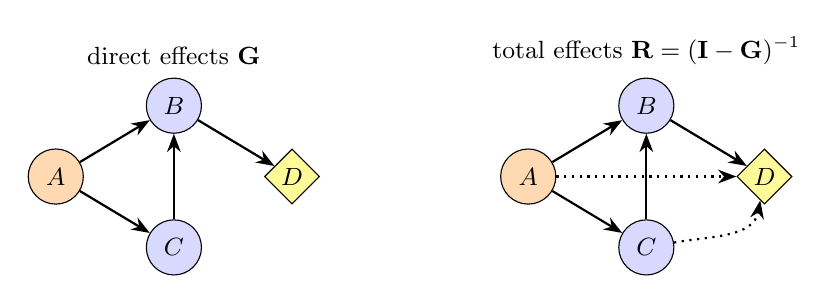
\begin{tikzpicture}[>=Stealth, every node/.style={font=\small}, nd/.style={circle, draw, fill=blue!15, minimum size=0.7cm}]
    \begin{scope}
      \node[above] at (1.5,1.3) {direct effects $\mG$};
      \node[nd, fill=orange!30] (a) at (0,0) {$A$};
      \node[nd] (b) at (1.5,0.9) {$B$};
      \node[nd] (c) at (1.5,-0.9) {$C$};
      \node[nd, fill=yellow!40, diamond, inner sep=1pt] (d) at (3.0,0) {$D$};
      \draw[->, thick] (a) -- (b); \draw[->, thick] (a) -- (c);
      \draw[->, thick] (c) -- (b); \draw[->, thick] (b) -- (d);
    \end{scope}
    \begin{scope}[xshift=6cm]
      \node[above] at (1.5,1.3) {total effects $\mR=(\mI-\mG)^{-1}$};
      \node[nd, fill=orange!30] (a) at (0,0) {$A$};
      \node[nd] (b) at (1.5,0.9) {$B$};
      \node[nd] (c) at (1.5,-0.9) {$C$};
      \node[nd, fill=yellow!40, diamond, inner sep=1pt] (d) at (3.0,0) {$D$};
      \draw[->, thick] (a) -- (b); \draw[->, thick] (a) -- (c);
      \draw[->, thick] (c) -- (b); \draw[->, thick] (b) -- (d);
      \draw[->, dotted, thick] (a) -- (d);
      \draw[->, dotted, thick] (c) to[out=10, in=-100] (d);
    \end{scope}
  \end{tikzpicture}
  \caption{Direct and total effects. Left, a network of direct causal effects in which a transcription factor $A$ regulates genes $B$ and $C$, $C$ regulates $B$, and $B$ affects a trait $D$. Right, the total effects estimated by pairwise MR include indirect effects (dotted), such as $A$ on $D$ through $B$, and $A$ on $B$ both directly and through $C$.}
  \label{fig:networks}
\end{figure}

A linear structural model relates the two. Let $\mY\in\R^{N\times D}$ hold $D$ phenotypes for $N$ individuals and $\mG\in\R^{D\times D}$ the direct effects, with $G_{ij}$ the effect of phenotype $i$ on phenotype $j$ and $G_{ii}=0$. Each phenotype is a linear function of the others plus external perturbations $\mE\in\R^{N\times D}$, which include the effects of genetic instruments and environment,
\begin{equation}
  \mY = \mY\mG + \mE \quad\Rightarrow\quad \mY(\mI-\mG) = \mE \quad\Rightarrow\quad \mY = \mE(\mI-\mG)^{-1}.
\end{equation}
A unit perturbation of phenotype $i$ (row vector $\mE$ with a one in position $i$) therefore changes phenotype $j$ by $[(\mI-\mG)^{-1}]_{ij}$, the total effect. When the network has no feedback loops strong enough to make the series diverge,
\begin{equation}
  (\mI-\mG)^{-1} = \mI + \mG + \mG^2 + \mG^3 + \cdots,
\end{equation}
and $[\mG^2]_{ij}=\sum_kG_{ik}G_{kj}$ sums the paths of length two from $i$ to $j$. In the network of Figure~\ref{fig:networks}, the total effect of $A$ on $B$ is $G_{AB}+G_{AC}G_{CB}$, the direct edge plus the path through $C$, and the total effect of $A$ on $D$ is $(G_{AB}+G_{AC}G_{CB})G_{BD}$.

MR estimates the total effect of a perturbation that changes $i$ by one unit, so the matrix of MR estimates is $\mR=\mD^{-1}(\mI-\mG)^{-1}$ with $\mD$ the diagonal of $(\mI-\mG)^{-1}$, normalizing each row so that $R_{ii}=1$. Then $\mR^{-1}=(\mI-\mG)\mD$, whose off-diagonal entries are $-G_{ij}D_{jj}$ and diagonal entries $D_{ii}$. A sparse network $\mG$ therefore means a sparse inverse of $\mR$, and the direct effects are recovered as $G_{ij}=-[\mR^{-1}]_{ij}/[\mR^{-1}]_{jj}$. Inverting a noisy estimate $\hat\mR$ directly amplifies the noise, so bimmer~\citep{brown2020bimmer} and its successor inspre~\citep{brown2023inspre} solve a regularized problem,
\begin{equation}
  \min_{\mU,\mV}\ \sum_{i,j}w_{ij}\big(\hat R_{ij}-U_{ij}\big)^2 + \lambda\|\mV\|_1 \quad\text{subject to}\quad \mU\mV=\mI,
\end{equation}
where $\mU\in\R^{D\times D}$ is a denoised version of $\hat\mR$, $\mV=\mU^{-1}$ is its sparse inverse, $w_{ij}\geq0$ are weights reflecting the precision of each MR estimate (zero for missing entries), and $\|\mV\|_1=\sum_{ij}|V_{ij}|$. The problem is biconvex (convex in $\mU$ for fixed $\mV$ and vice versa) and is solved with the alternating direction method of multipliers (ADMM)~\citep{boyd2011admm}. It is the directed analogue of the graphical lasso of Chapter 9~\citep{friedman2008}, which finds a sparse inverse of a covariance matrix, and $\lambda$ is chosen by a stability criterion adapted from StARS~\citep{liu2010stars}. In simulations of random, hub-like and scale-free directed networks, this approach recovers the network much more accurately than estimating each node's parents by sparse regression on pairwise MR estimates. Applied with CRISPR knockdowns as the perturbations instead of genetic instruments, the same method estimates gene regulatory networks from Perturb-seq data~\citep{brown2023inspre}.

%======================================================================
\section{Summary}
%======================================================================

\begin{itemize}
  \item Molecular QTLs are associations between genotype and molecular phenotypes such as expression (eQTLs), splicing (sQTLs) and chromatin accessibility (caQTLs). They help interpret GWAS loci, most of which are non-coding, by suggesting causal genes, tissues and cell types, as in the \textit{FTO} locus, where the obesity variants regulate \textit{IRX3} and \textit{IRX5} in adipocyte progenitors.
  \item eQTLs are mapped by linear regression of normalized expression on genotype, usually for SNPs within 1\,Mb of each gene. Multiple testing is handled at two levels: within a gene by Bonferroni or permutation, which accounts for LD, and across genes by FDR control.
  \item Technical and biological confounders affect many genes at once and can be estimated as hidden factors with a factor model with an ARD prior (PEER) or by PCA. Regressing them out greatly increases power for cis-eQTLs but can remove trans signals and context-specific biology.
  \item Cis-eQTLs are common, large and easy to find with tens to hundreds of individuals; trans-eQTLs are small and need thousands. LD makes the causal variant hard to identify; fine-mapping and genome-wide annotation enrichment, which shows causal variants concentrated in accessible chromatin near the TSS, help.
  \item Allele-specific expression compares the two haplotypes within an individual, a built-in control for environmental and technical variation that isolates cis effects. Overdispersed counts are modelled with the beta-binomial (allelic counts) and negative binomial (total counts), and combining the two signals gains power, especially in small samples. QQ plots check calibration.
  \item Tissue atlases show that most genes have cis-eQTLs, often several, that eQTLs are mostly either shared across tissues or specific to a few, and that comparing significance between tissues is misleading; mash models effects jointly. Cell type composition shapes bulk eQTLs, and interaction models can recover cell type-specific effects.
  \item Colocalization tests whether a GWAS and an eQTL signal share a causal variant; TWAS associates genetically predicted expression with a trait; Mendelian randomization estimates causal effects using SNPs as instrumental variables, with Egger and related methods relaxing the no-pleiotropy assumption. Extending MR to many phenotypes leads to sparse causal network inference.
\end{itemize}

%======================================================================
\section*{Exercises}
%======================================================================

\begin{enumerate}
  \item Show that under the null, with $M$ independent SNPs, $\Pr(p_{\min}\leq t)=1-(1-t)^M$, and that the Bonferroni threshold $t=0.05/M$ gives a family-wise error rate between 0.0488 and 0.05 for all $M\geq1$.
  \item Starting from~\eqref{eq:betabinom}, show that $\Pr(y\mid d,\mu,c)\to\binom{d}{y}\mu^y(1-\mu)^{d-y}$ as $c\to\infty$ with $\mu$ fixed. Show similarly that $\NB(y\mid m,\phi)\to\Pois(y\mid m)$ as $\phi\to\infty$.
  \item In the combined model~\eqref{eq:cht}, suppose all individuals are heterozygous at the test SNP and the dispersions are known. Write the log likelihood as a function of $\theta_R$ and $\theta_A$ and explain which terms carry the between-individual and which the within-individual information. What changes if no individual is heterozygous?
  \item Derive Wakefield's approximate Bayes factor~\eqref{eq:abf-12}. Show that for fixed $z_m$ it decreases to zero as $W\to\infty$, and explain why.
  \item Under the null $\vz\sim\Normal(\vzero,\mSigma)$, show that $z_{\text{TWAS}}$ in~\eqref{eq:twas} is standard normal. Show that if $\hat\vw$ has a single non-zero entry, $z_{\text{TWAS}}=\pm z_m$ for that SNP.
  \item For the network in Figure~\ref{fig:networks}, write $\mG$ with symbolic entries, compute $(\mI-\mG)^{-1}$ and check the total effects given in the text. Verify that $\mG$ is nilpotent, so the series for $(\mI-\mG)^{-1}$ terminates.
  \item Simulate genotypes for 300 individuals at 500 SNPs with LD (for example by copying segments of a few founder haplotypes) and expression for 1000 genes, 10\% of which have one causal cis SNP. Call eGenes at 5\% FDR using Bonferroni-adjusted and permutation-based gene-level p values with Benjamini-Hochberg, and compare the number of discoveries.
\end{enumerate}
.
\documentclass[11pt]{book}
\usepackage[T1]{fontenc}
\usepackage{lmodern}
\usepackage{microtype}
\usepackage[margin=1.1in]{geometry}
\usepackage{amsmath,amssymb,bm}
\usepackage{graphicx}
\usepackage{booktabs}
\usepackage{multirow}
\usepackage{xcolor}
\usepackage{caption}
\usepackage{subcaption}
\usepackage{algorithm}
\usepackage{algpseudocode}
\usepackage{tikz}
\usetikzlibrary{arrows.meta,positioning,calc,decorations.pathreplacing,decorations.pathmorphing,shapes.geometric,fit}
\usepackage[numbers,sort&compress]{natbib}
\usepackage{hyperref}
\hypersetup{colorlinks=true,linkcolor=blue!50!black,citecolor=blue!50!black,urlcolor=blue!50!black}
\graphicspath{{figures/}}

\begin{document}
\setcounter{chapter}{11}
% Chapter 12: molecular quantitative trait loci.
% Requires: amsmath, amssymb, bm, graphicx, booktabs, multirow, subcaption,
% tikz (arrows.meta, positioning, calc, decorations.pathreplacing, decorations.pathmorphing, shapes.geometric, fit), natbib.
% Computed figures are produced by scripts/make_figures.py; figures/slides/ holds figures taken from the lecture slides.

\providecommand{\R}{\mathbb{R}}
\providecommand{\E}{\mathbb{E}}
\providecommand{\Normal}{\mathcal{N}}
\providecommand{\argmax}{\operatorname*{arg\,max}}
\providecommand{\argmin}{\operatorname*{arg\,min}}
\providecommand{\vy}{\mathbf{y}}
\providecommand{\vx}{\mathbf{x}}
\providecommand{\mX}{\mathbf{X}}
\providecommand{\mI}{\mathbf{I}}
\providecommand{\vb}{\boldsymbol{\beta}}
\providecommand{\veps}{\boldsymbol{\epsilon}}
\providecommand{\vp}{\mathbf{p}}
\providecommand{\vg}{\mathbf{g}}
\providecommand{\ind}{\mathbf{1}}
% new in this chapter
\providecommand{\mY}{\mathbf{Y}}
\providecommand{\mW}{\mathbf{W}}
\providecommand{\mE}{\mathbf{E}}
\providecommand{\mS}{\mathbf{S}}
\providecommand{\mF}{\mathbf{F}}
\providecommand{\mG}{\mathbf{G}}
\providecommand{\mR}{\mathbf{R}}
\providecommand{\mU}{\mathbf{U}}
\providecommand{\mV}{\mathbf{V}}
\providecommand{\mD}{\mathbf{D}}
\providecommand{\mA}{\mathbf{A}}
\providecommand{\mSigma}{\boldsymbol{\Sigma}}
\providecommand{\vw}{\mathbf{w}}
\providecommand{\vz}{\mathbf{z}}
\providecommand{\va}{\mathbf{a}}
\providecommand{\vs}{\mathbf{s}}
\providecommand{\vf}{\mathbf{f}}
\providecommand{\vbhat}{\hat{\mathbf{b}}}
\providecommand{\vbb}{\mathbf{b}}
\providecommand{\vm}{\mathbf{m}}
\providecommand{\ve}{\mathbf{e}}
\providecommand{\vlambda}{\boldsymbol{\lambda}}
\providecommand{\vzero}{\mathbf{0}}
\providecommand{\diag}{\operatorname{diag}}
\providecommand{\Gam}{\operatorname{Gamma}}
\providecommand{\Var}{\operatorname{Var}}
\providecommand{\Cov}{\operatorname{Cov}}
\providecommand{\Bin}{\operatorname{Bin}}
\providecommand{\BetaBin}{\operatorname{BetaBin}}
\providecommand{\NB}{\operatorname{NB}}
\providecommand{\Pois}{\operatorname{Pois}}
\providecommand{\BetaDist}{\operatorname{Beta}}
\providecommand{\BetaFn}{\mathrm{B}}

\chapter{Molecular quantitative trait loci}
\label{ch:molqtl}

Chapter 11 showed that genome-wide association studies (GWAS) have found tens of thousands of genomic regions associated with traits and diseases, and that most of the associated variants do not change the sequence of a protein. They are thought to act by changing gene regulation: when, where and how much a gene is expressed or how its RNA is spliced. This chapter is about the main tool for studying that regulation in human populations, the \emph{molecular quantitative trait locus} (molecular QTL): a genetic variant associated with a molecular phenotype such as the expression level of a gene. We cover how molecular QTL studies are designed and analysed, how to remove the hidden confounders that plague large omics data sets, how allele-specific measurements give a second, better controlled view of the same genetic effects, what the large tissue atlases have taught us, and finally how molecular QTLs are combined with GWAS to propose causal genes, using colocalization, transcriptome-wide association studies and Mendelian randomization.

%======================================================================
\section{From GWAS loci to molecular mechanisms}
%======================================================================

\subsection{The FTO locus}

The strongest common genetic association with obesity, in adults and in children~\citep{bradfield2012}, lies in a region of chromosome 16 that contains the gene \textit{FTO}. The associated variants fall in an intron of \textit{FTO}, so the locus was named after it and \textit{FTO} was assumed to be the causal gene. \citet{claussnitzer2015} worked through this locus in detail, and their analysis uses many of the ideas of this and earlier chapters, so it is a good place to start.

Figure~\ref{fig:fto_locus-12}a is a LocusZoom plot of the association with body mass index (BMI). Many variants are strongly associated, and their colour, the linkage disequilibrium (LD) $r^2$ with the lead variant, shows that they are all correlated with each other: genetic association alone cannot say which of them is causal (Chapter 11). The authors next looked at chromatin states from the Roadmap Epigenomics project, the ChromHMM annotation of Chapter 6, across many cell types (Figure~\ref{fig:fto_locus-12}b). The associated region is in an active, enhancer-like state in mesenchymal cells, the progenitors of connective tissue that include adipocytes (fat cells) and their precursors, and much less active elsewhere. That points to adipocyte progenitors as the cell type in which the variants act.

\begin{figure}[!htbp]
  \centering
  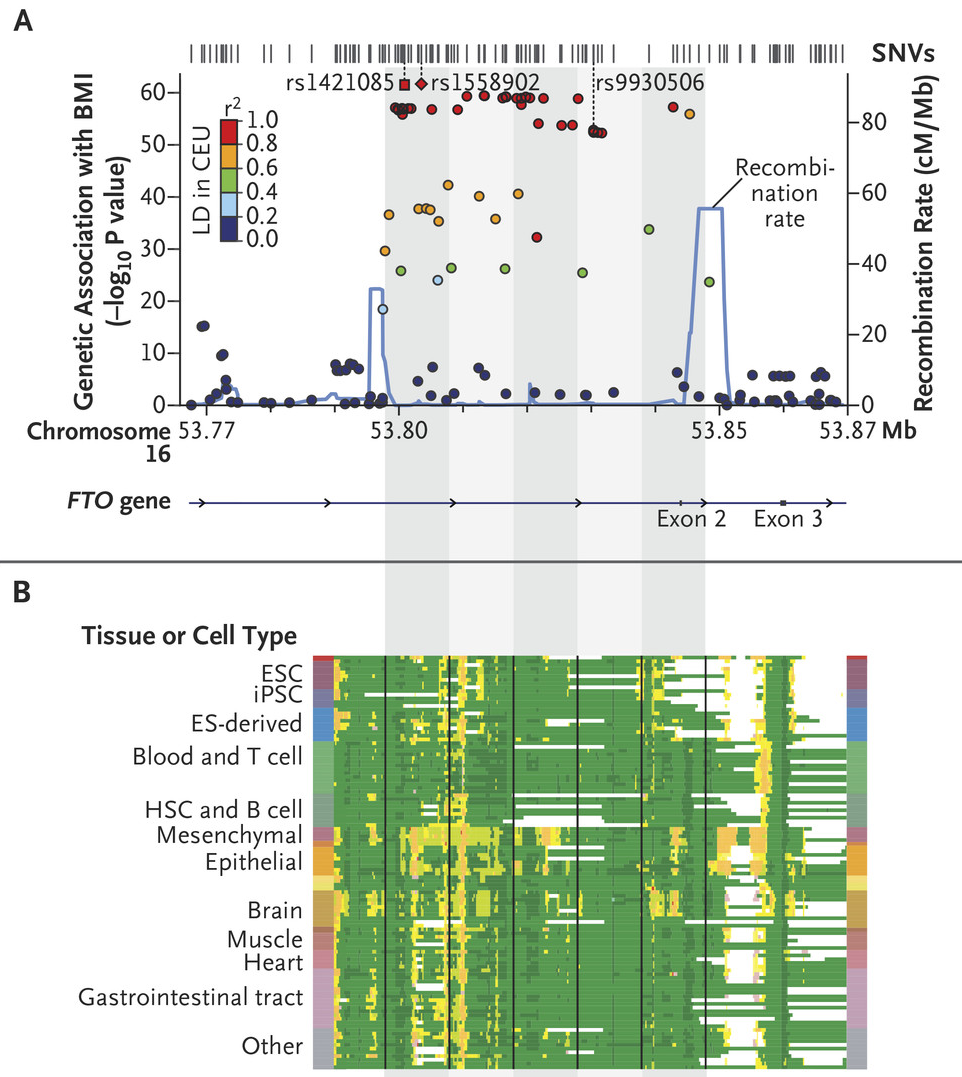
\includegraphics[width=0.72\linewidth]{slides/fto_locus.png}
  \caption{The \textit{FTO} obesity locus. (a) Association of variants with BMI ($-\log_{10}$ p value) along chromosome 16, coloured by LD ($r^2$ in European-ancestry samples) with the lead variants, with the recombination rate and the \textit{FTO} gene below. (b) Roadmap Epigenomics chromatin states across tissues and cell types for the same region; the associated region is in an active enhancer state (yellow) in mesenchymal cells. Reproduced from \citet{claussnitzer2015}.}
  \label{fig:fto_locus-12}
\end{figure}

Which gene does the enhancer regulate? The region contains several genes besides \textit{FTO} (Figure~\ref{fig:fto_expression}, top). In pre-adipocytes from people with the risk and non-risk genotypes, expression of \textit{FTO} itself did not differ, but expression of \textit{IRX3} and \textit{IRX5}, which lie 0.5 and 1.2 megabases (Mb) away, was higher with the risk genotype (Figure~\ref{fig:fto_expression}, bottom). The effect was specific to pre-adipocytes. \textit{IRX3} and \textit{IRX5} encode transcription factors that shift the fate of adipocyte progenitors: higher expression makes a progenitor more likely to become a white adipocyte, which stores lipid, and less likely to become a beige adipocyte, which burns lipid to produce heat (thermogenesis). The risk allele therefore tilts the balance toward fat storage. The authors identified a single nucleotide variant, rs1421085, that disrupts a binding site for the repressor ARID5B, and showed that editing it with CRISPR switched the expression of \textit{IRX3} and \textit{IRX5} and the thermogenic programme. Storing more fat may have been advantageous when food was scarce; in an environment with abundant food the same variant is maladaptive.

\begin{figure}[!htbp]
  \centering
  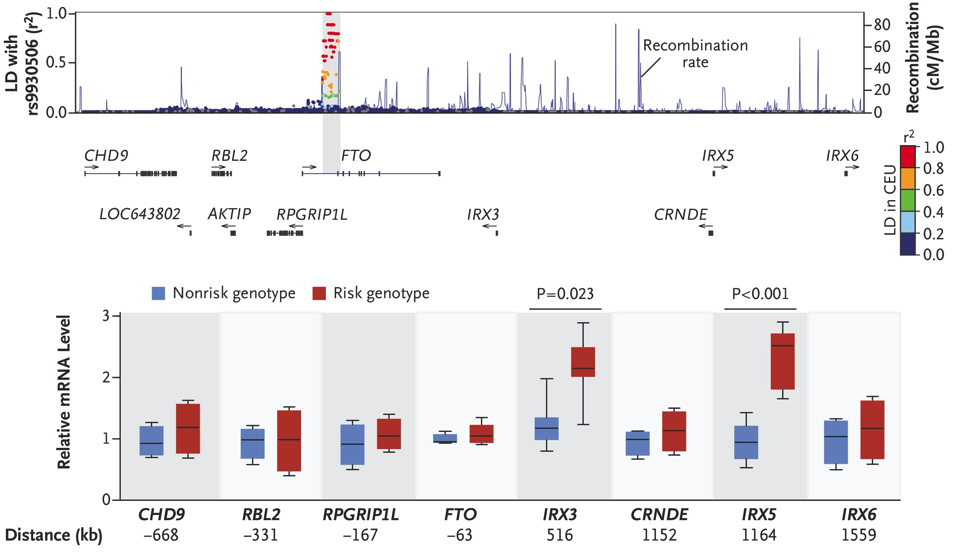
\includegraphics[width=0.85\linewidth]{slides/fto_expression.png}
  \caption{Genes near the \textit{FTO} association (top; LD with the lead variant rs9930506 and recombination rate) and their expression in human pre-adipocytes from carriers of the risk and non-risk genotypes (bottom). Only \textit{IRX3} and \textit{IRX5}, more than 500 kb from the associated variants, differ. Distances are from the associated region. Reproduced from \citet{claussnitzer2015}.}
  \label{fig:fto_expression}
\end{figure}

The example illustrates three general difficulties of interpreting a GWAS locus, which recur throughout this chapter: finding the \emph{causal variant} among many correlated ones, finding the \emph{cell type} (and possibly the cell state) in which it acts, and finding the \emph{target gene}, which need not be the nearest gene. It also shows why we care. Knowing that the locus acts through \textit{IRX3} and \textit{IRX5} in adipocyte progenitors suggests interventions, such as reducing their activity to favour beige adipocytes, and more generally tells us about the human biology of a disease without a clinical trial.

\subsection{Molecular mediators of genetic effects}

The logic of the \textit{FTO} analysis is that of mediation (Figure~\ref{fig:mediation}). A genetic variant is associated with disease risk, and we want to find the molecular changes, such as a change in the expression of a gene, that lie on the causal path between them. Genetic variation is useful here because it gives us one route to causality: genotypes are fixed at conception, so an association between a variant and a molecular trait cannot be caused by the trait. The reverse arrows in Figure~\ref{fig:mediation} are a reminder that the data do not have to follow the simple chain. A variant can raise disease risk through some other route, and the disease can then change gene expression as the body responds to it, so an association between disease and expression measured in patients need not be causal for the disease.

\begin{figure}[!htbp]
  \centering
  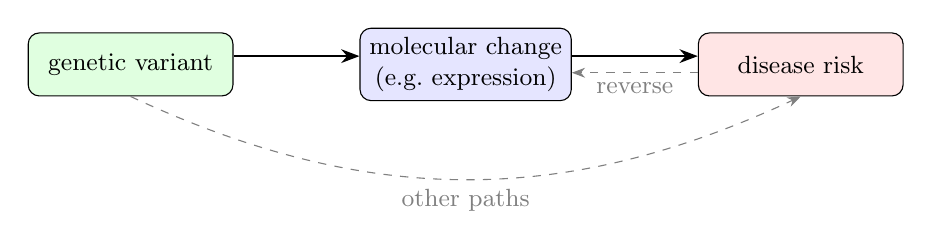
\begin{tikzpicture}[>=Stealth, every node/.style={font=\small}, box/.style={draw, rounded corners, minimum width=2.6cm, minimum height=0.8cm, align=center}]
    \node[box, fill=green!12] (g) {genetic variant};
    \node[box, fill=blue!10, right=1.6cm of g] (m) {molecular change\\(e.g.\ expression)};
    \node[box, fill=red!10, right=1.6cm of m] (d) {disease risk};
    \draw[->, thick] ([yshift=3pt]g.east) -- ([yshift=3pt]m.west);
    \draw[->, thick] ([yshift=3pt]m.east) -- ([yshift=3pt]d.west);
    \draw[->, dashed, gray] ([yshift=-3pt]d.west) -- ([yshift=-3pt]m.east) node[midway, below] {reverse};
    \draw[->, dashed, gray] (g.south) to[out=-25, in=-155] node[midway, below] {other paths} (d.south);
  \end{tikzpicture}
  \caption{Molecular mediators of genetic effects. We would like to find molecular changes on the causal path from a variant to disease. Disease can also change molecular phenotypes (reverse causation), and a variant can affect disease through other paths.}
  \label{fig:mediation}
\end{figure}

%======================================================================
\section{Molecular QTLs}
%======================================================================

\subsection{Layers of omics}

Any molecular readout that can be measured at scale across many individuals can be associated with genotype. The readouts follow the layers of gene regulation met in earlier chapters:
\begin{itemize}
  \item the \emph{genome}: the genetic variants themselves;
  \item the \emph{epigenome}: transcription factor binding (ChIP-seq), DNA methylation (bisulfite sequencing or, more cheaply and at larger scale, methylation arrays), chromatin accessibility (ATAC-seq, DNase-seq) and histone modifications;
  \item the \emph{transcriptome}: gene expression and splicing (RNA-seq);
  \item the \emph{proteome}: protein levels, now measured for a few thousand proteins in tens of thousands of people with affinity-based assays;
  \item the \emph{metabolome}: small molecules in cells or blood.
\end{itemize}
A QTL for each readout gets its own name (Table~\ref{tab:qtl_types}). The most studied are expression QTLs (eQTLs). A gene with at least one significant eQTL is an \emph{eGene}, a variant significantly associated with its expression is an \emph{eVariant}, and the most significant variant for a gene is the \emph{lead} or \emph{top} variant. The terms are awkward but widely used.

\begin{table}[!htbp]
  \centering
  \caption{Types of molecular QTL. Each associates genotype at a variant with a molecular phenotype measured across individuals.}
  \label{tab:qtl_types}
  \small
  \begin{tabular}{p{3.6cm}p{5.6cm}p{3.6cm}}
    \toprule
    QTL & phenotype & typical assay \\
    \midrule
    eQTL (expression) & RNA level of a gene or transcript & RNA-seq \\
    sQTL (splicing) & inclusion ratio of an exon, ratio of isoforms, intron usage & RNA-seq \\
    pQTL (protein) & protein level of a gene & mass spectrometry, affinity assays \\
    meQTL (methylation) & methylation ratio of a CpG site & bisulfite sequencing, arrays \\
    caQTL (chromatin accessibility) & accessibility of a region & ATAC-seq, DNase-seq \\
    hQTL (histone modification) & ChIP-seq peak height of a histone mark & ChIP-seq \\
    \bottomrule
  \end{tabular}
\end{table}

\subsection{Approaches to interpreting GWAS variants}

QTL mapping is one of several ways to interpret a GWAS association~\citep{albert2015}. The simplest is \emph{annotation overlap}: does the variant fall in a gene, a conserved region, or a ChromHMM promoter or enhancer state in a relevant cell type, as in the \textit{FTO} example? A second is \emph{predictive models}, which score how likely a variant is to be functional, either from annotations and conservation or, as in Chapters 2 and 3, from sequence by \emph{in silico} mutagenesis of a deep learning model. A third is \emph{QTL mapping}, the subject of this chapter, which measures the effect of the variant on a molecular phenotype directly in a population. A fourth, \emph{outlier detection}, looks for individuals whose expression is far outside the population distribution and asks whether they carry rare variants; we return to rare variants in the next chapter.

Why not simply predict the effect of each variant from its annotation? For coding variants the consequences are reasonably well understood. A nonsense variant introduces a premature stop codon, a frameshift changes the reading frame, and both usually truncate the protein or trigger nonsense-mediated decay of the RNA. A missense variant changes one amino acid, which may alter the protein's structure or function but not its dosage. For non-coding variants the picture is murkier. Variants in the 5$'$ untranslated region (UTR) can change how efficiently the RNA is translated, variants in the 3$'$ UTR can change its stability, variants near splice sites can change splicing, which can change either the protein sequence or, through decay of a non-productive isoform, the dosage, and variants in promoters and enhancers can change transcription. Most of these variants have no effect at all. Tools exist that label each variant with its possible consequences, but there are few experimentally labelled examples from which to learn which non-coding variants matter. QTL mapping supplies noisy but genome-wide evidence of exactly that.

%======================================================================
\section{Mapping expression QTLs}
%======================================================================

\subsection{Study design}

An eQTL study needs two measurements on the same individuals (Figure~\ref{fig:study_design}). One is genotype, from DNA sequencing or, more cheaply, a genotyping array followed by imputation (Chapter 11). The other is a molecular readout from one or several tissues, most often RNA-seq. RNA-seq gives two kinds of genetic signal. Comparing expression levels across individuals with different genotypes gives eQTLs. Within an individual who is heterozygous at a variant in the transcribed sequence, reads carrying each allele can be counted separately, which gives \emph{allelic expression} (AE), the subject of Section~\ref{sec:ase}.

\begin{figure}[!htbp]
  \centering
  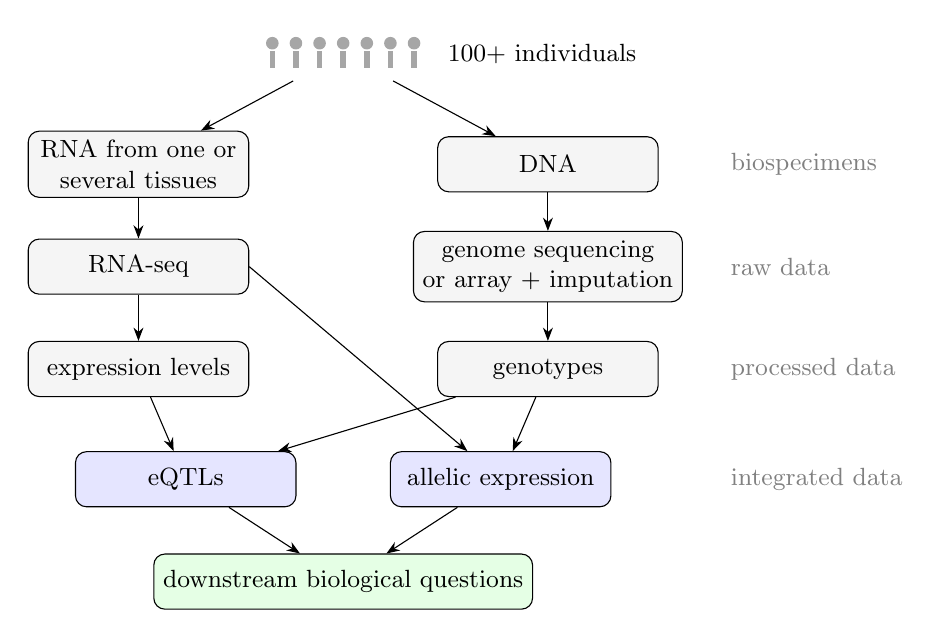
\begin{tikzpicture}[>=Stealth, every node/.style={font=\small}, box/.style={draw, rounded corners, minimum width=2.8cm, minimum height=0.7cm, align=center, fill=gray!8}]
    \node (ppl) at (2.6,0) {\tikz{\foreach \x in {0,0.3,...,2.1} {\fill[gray!70] (\x,0.32) circle (0.08); \draw[gray!70, line width=2pt] (\x,0.22) -- (\x,0);}}};
    \node[right=0.1cm of ppl] {100+ individuals};
    \node[box] (rna) at (0,-1.4) {RNA from one or\\several tissues};
    \node[box] (dna) at (5.2,-1.4) {DNA};
    \node[box] (rseq) at (0,-2.7) {RNA-seq};
    \node[box] (gseq) at (5.2,-2.7) {genome sequencing\\or array + imputation};
    \node[box] (expr) at (0,-4.0) {expression levels};
    \node[box] (geno) at (5.2,-4.0) {genotypes};
    \node[box, fill=blue!10] (eqtl) at (0.6,-5.4) {eQTLs};
    \node[box, fill=blue!10] (ae) at (4.6,-5.4) {allelic expression};
    \node[box, fill=green!10] (down) at (2.6,-6.7) {downstream biological questions};
    \draw[->] (ppl) -- (rna); \draw[->] (ppl) -- (dna);
    \draw[->] (rna) -- (rseq); \draw[->] (dna) -- (gseq);
    \draw[->] (rseq) -- (expr); \draw[->] (gseq) -- (geno);
    \draw[->] (expr) -- (eqtl); \draw[->] (geno) -- (eqtl);
    \draw[->] (rseq.east) -- (ae); \draw[->] (geno) -- (ae);
    \draw[->] (eqtl) -- (down); \draw[->] (ae) -- (down);
    \node[right, gray, align=left] at (7.4,-1.4) {biospecimens};
    \node[right, gray] at (7.4,-2.7) {raw data};
    \node[right, gray] at (7.4,-4.0) {processed data};
    \node[right, gray] at (7.4,-5.4) {integrated data};
  \end{tikzpicture}
  \caption{Design of a molecular QTL study. Genotypes and RNA-seq (or another molecular assay) are measured on the same individuals. Expression levels compared across genotypes give eQTLs; read counts for the two alleles within heterozygous individuals give allelic expression.}
  \label{fig:study_design}
\end{figure}

Sample sizes are modest compared with GWAS. The smallest eQTL studies have around 50 individuals, typical ones a few hundred, well-powered ones around 1000, and meta-analyses tens of thousands. A large GWAS of a disease or of height, by contrast, has hundreds of thousands of individuals. eQTL studies can afford to be smaller because the effects are larger, often a substantial fraction of a gene's expression variance, and, as we discuss next, because they only search a small part of the genome for each gene.

\subsection{The association model}

Let $N$ be the number of individuals and $y_n$ the normalized expression of one gene in individual $n$, for example log counts per million after library size normalization, often followed by an inverse normal transform across individuals. Let $g_n\in\{0,1,2\}$ be the genotype of individual $n$ at one biallelic SNP, coded as the number of copies of the alternative (or minor) allele. Imputed genotypes give an expected count, or \emph{dosage}, in $[0,2]$. The standard model is the linear regression of Chapter 1,
\begin{equation}
  y_n = \mu + \beta g_n + \vx_n^\top\boldsymbol{\delta} + \epsilon_n, \qquad \epsilon_n\sim\Normal(0,\sigma^2),
  \label{eq:eqtl_lm}
\end{equation}
where $\mu$ is the intercept, $\beta$ is the eQTL effect size, $\vx_n\in\R^C$ is a vector of $C$ covariates (sex, genotype principal components for ancestry, technical factors, and the hidden factors of Section~\ref{sec:hidden}) with coefficients $\boldsymbol{\delta}\in\R^C$, and $\sigma^2$ is the noise variance. Coding the genotype as an allele count assumes the two copies of the gene act additively: the heterozygote is halfway between the two homozygotes. This is a reasonable default, since what happens on one chromosome is mostly independent of what happens on the other, and it is the same additive model used for GWAS. We test $H_0:\beta=0$ with the $t$ statistic $\hat\beta/\widehat{\text{se}}(\hat\beta)$, which has a $t$ distribution with $N-2-C$ degrees of freedom under the null. Figure~\ref{fig:eqtl_example} shows a simulated eQTL.

\begin{figure}[!htbp]
  \centering
  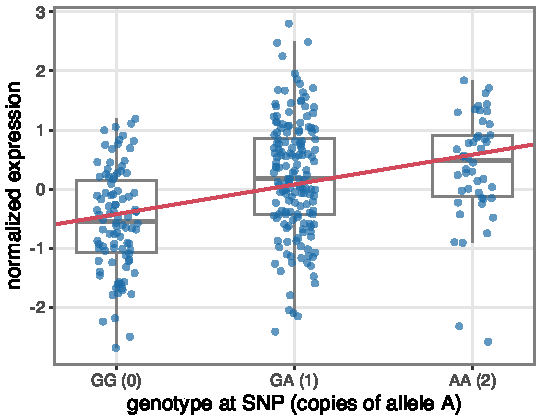
\includegraphics[width=0.5\linewidth]{eqtl_example.pdf}
  \caption{A simulated eQTL in $N=300$ individuals: normalized expression of a gene against genotype at a nearby SNP, with the least-squares fit of~\eqref{eq:eqtl_lm} (red). Each copy of allele A raises expression by about half a standard deviation.}
  \label{fig:eqtl_example}
\end{figure}

When individuals are related, or the cohort has strong population structure, the linear mixed models of Chapter 11 replace~\eqref{eq:eqtl_lm}, with a random effect whose covariance is the genetic relatedness matrix. Simple regression remains the most common choice, and fast matrix implementations test all SNP-gene pairs in a study in minutes~\citep{shabalin2012}.

\subsection{Cis windows and the testing burden}

Which SNPs should be tested for each gene? Empirically, by far the strongest genetic effects on a gene's expression come from variants close to it. The usual practice is to test every SNP within a window, typically 1\,Mb on either side of the transcription start site (TSS). These are \emph{cis}-eQTLs. With roughly one common SNP per kilobase, a 2\,Mb window holds of the order of $M=2000$ SNPs, compared with millions for a GWAS. For chromatin phenotypes such as histone marks or accessibility, genetic effects are even more local, and the window is often only the peak itself plus a few kilobases.

The smaller search space is the second reason eQTL studies work at modest sample size. With Bonferroni correction (below), a GWAS needs a p value below $0.05/(3\times10^6)\approx 1.7\times10^{-8}$, while a single gene's cis window needs $0.05/2000=2.5\times10^{-5}$.

\subsection{Multiple testing at two levels}

Multiple testing in an eQTL study has two levels. For each gene we test $M$ SNPs, and we do this for $P$ genes, typically $P\approx 20{,}000$. The usual strategy is first to compute one p value per gene for the null hypothesis that no SNP in its window affects it, and then to control the false discovery rate across genes.

\paragraph{Within a gene.} Let $p_1,\dots,p_M$ be the p values of the SNPs in the window, and $p_{\min}=\min_m p_m$. Under the null each $p_m$ is uniform on $[0,1]$, so for a threshold $t$ the union bound gives
\begin{equation}
  \Pr(p_{\min}\leq t) = \Pr\Big(\bigcup_{m=1}^M\{p_m\leq t\}\Big) \leq \sum_{m=1}^M\Pr(p_m\leq t) = Mt.
\end{equation}
Choosing $t=0.05/M$ controls the probability of any false positive in the window at 5\%; this is the \emph{Bonferroni correction}, and $\min(1,Mp_{\min})$ is the Bonferroni-adjusted gene-level p value. The bound is close to tight when the tests are independent, since then $\Pr(p_{\min}\leq t)=1-(1-t)^M\approx Mt$ for small $t$. SNPs in a cis window are far from independent: LD makes neighbouring SNPs proxies for each other, so the window contains fewer effectively independent tests than $M$, and Bonferroni is conservative.

\emph{Permutation} gives the exact null distribution of $p_{\min}$ for the window. Permuting the expression values across individuals (equivalently, permuting genotype vectors as whole rows, so that LD between SNPs is preserved) breaks any association between genotype and expression while keeping the LD structure and the distribution of expression. For permutations $b=1,\dots,B$ we recompute $p_{\min}^{(b)}$, and the permutation p value is
\begin{equation}
  p_{\text{perm}} = \frac{1+\sum_{b=1}^B\ind\big[p_{\min}^{(b)}\leq p_{\min}\big]}{B+1}.
\end{equation}
Any statistic can be used in place of $p_{\min}$, for example the maximum $|r|$ or $R^2$. Permutation has to recompute the regressions $B$ times for every gene, which is expensive when small gene-level p values must be resolved; FastQTL~\citep{ongen2016} reduces the cost by fitting a beta distribution to a modest number of permuted $p_{\min}$ values and extrapolating. Covariates complicate permutation, because permuting $y$ also breaks its relation to the covariates; the usual remedy is to regress the covariates out of expression first and permute the residuals. Figure~\ref{fig:permutation_null} compares the permutation null of $p_{\min}$ for a window of independent SNPs and for a window with realistic LD. With LD, the 5\% permutation threshold is several times less stringent than Bonferroni, as if the window contained only a quarter of its SNPs.

\begin{figure}[!htbp]
  \centering
  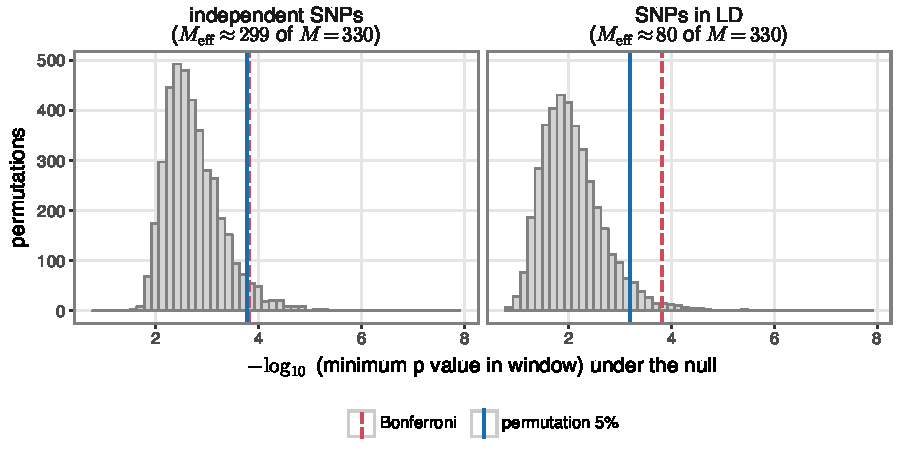
\includegraphics[width=0.85\linewidth]{permutation_null.pdf}
  \caption{Permutation null distribution of the minimum p value across a cis window of $M=330$ SNPs in $N=200$ individuals, from 4000 permutations of a null expression vector. Left, SNPs simulated independently; right, SNPs simulated with block-like LD. The Bonferroni threshold $0.05/M$ (red, dashed) matches the permutation 5\% threshold (blue) for independent SNPs but is conservative with LD. $M_{\text{eff}}=0.05/t_{\text{perm}}$ is the number of independent tests that would give the same threshold.}
  \label{fig:permutation_null}
\end{figure}

\paragraph{Across genes.} Controlling the probability of any false positive across $20{,}000$ genes would be very stringent. Instead we control the \emph{false discovery rate} (FDR), the expected fraction of false positives among the genes we call significant,
\begin{equation}
  \text{FDR} = \E\left[\frac{V}{\max(R,1)}\right],
\end{equation}
where $R$ is the number of genes called eGenes and $V$ the number of those that are null. If we report 5000 eGenes at 10\% FDR, we expect about 500 to be false positives, though we do not know which. The Benjamini-Hochberg (BH) procedure~\citep{benjamini1995} takes the $P$ gene-level p values, sorts them, $p_{(1)}\leq\dots\leq p_{(P)}$, finds the largest $k$ such that
\begin{equation}
  p_{(k)} \leq \frac{k}{P}q,
\end{equation}
and calls the genes with the $k$ smallest p values significant. For independent (or positively dependent) tests this controls the FDR at level $q$. One way to see why: if all $P$ genes were null, about $Pt$ of them would have p values below $t$, so with $k$ genes below $t=p_{(k)}$ the estimated fraction of false discoveries is $Pp_{(k)}/k$, and BH picks the largest set for which this estimate is at most $q$. The $q$-value approach~\citep{storey2003} also estimates the fraction of genes that are null, which gains power when many genes are eGenes. GTEx and most other studies apply the FDR procedure to permutation-based gene-level p values and then, within each eGene, call as eVariants the SNPs whose nominal p values fall below a gene-specific threshold derived from the gene-level cutoff.

%======================================================================
\section{Hidden confounders}
\label{sec:hidden}
%======================================================================

\subsection{Sources of unwanted variation}

Large omics data sets always contain variation that is not the biology we want to study. Some is technical: who prepared the samples, on which day, with which reagent batch, on which sequencing machine. Many eQTL studies use post-mortem tissue, where the \emph{ischaemic time} between death and preservation degrades RNA, and the RNA integrity number (RIN) measures the result. Some is biological but not of interest here: age, sex, environment, recent infections, and in bulk tissue the proportions of different cell types, which vary between people and between pieces of tissue. In GTEx, a study of almost 1000 post-mortem donors and around 50 tissues~\citep{gtex2020}, sample collection variables (ventilator use, ischaemic time, RIN), sequencing batch and library construction are each associated with the main axes of expression variation in many tissues, with $R^2$ up to about 0.3, and estimated cell type proportions are associated to a similar degree.

Such factors affect many genes at once. They do not usually create false eQTLs, because they are not associated with the genotype of a particular SNP, but they add noise to every test and so reduce power. Known factors can be included as covariates in~\eqref{eq:eqtl_lm}. Unknown ones have to be inferred from the expression data.

\subsection{PEER: a factor model for expression}

Chapter 8 introduced factor analysis, $\mY\approx\mX\mW^\top$, and its Bayesian version with an automatic relevance determination (ARD) prior. Because confounders affect many genes, they appear as low-rank structure in the expression matrix, and factor analysis is a natural way to estimate them. PEER (probabilistic estimation of expression residuals)~\citep{stegle2010,stegle2012} combines this with the genetic and known covariate effects in one model (Figure~\ref{fig:peer_model}).

Let $\mY\in\R^{N\times P}$ be the expression matrix of $N$ individuals and $P$ genes (the PEER paper writes the transpose, genes by individuals). The model decomposes it into four parts,
\begin{equation}
  \mY = \underbrace{\mS\mW_S^\top}_{\text{genotype}} + \underbrace{\mF\mW_F^\top}_{\text{known factors}} + \underbrace{\mX\mW^\top}_{\text{hidden factors}} + \mE,
  \label{eq:peer}
\end{equation}
where $\mS\in\{0,1,2\}^{N\times M}$ holds the genotypes of $M$ SNPs with effects $\mW_S\in\R^{P\times M}$; $\mF\in\R^{N\times C}$ holds $C$ measured covariates such as age, sex and batch, with coefficients $\mW_F\in\R^{P\times C}$; $\mX\in\R^{N\times K}$ holds $K$ hidden factors with loadings $\mW\in\R^{P\times K}$; and $\mE\in\R^{N\times P}$ is noise. Element-wise, for gene $p$ and individual $n$,
\begin{equation}
  y_{np}\sim\Normal\Big(\sum_m s_{nm}w^S_{pm}+\sum_c f_{nc}w^F_{pc}+\sum_{k=1}^K x_{nk}w_{pk},\ \tau_p^{-1}\Big),
\end{equation}
with a noise precision $\tau_p$ for each gene, as in factor analysis. The hidden-factor part has the priors of Chapter 8,
\begin{align}
  x_{nk}&\sim\Normal(0,1), & w_{pk}&\sim\Normal(0,\alpha_k^{-1}), & \alpha_k&\sim\Gam(a_\alpha,b_\alpha), & \tau_p&\sim\Gam(a_\tau,b_\tau).
  \label{eq:peer_priors}
\end{align}
The prior precision $\alpha_k$ is shared by all loadings of factor $k$. This is ARD again: if the data do not support factor $k$, $\alpha_k$ grows, the prior variance $1/\alpha_k$ of its loadings shrinks to zero, and the factor is switched off. To see how $\alpha_k$ is set, consider the terms of the log joint density that involve it,
\begin{multline}
  \sum_{p=1}^P\log\Normal(w_{pk}\mid0,\alpha_k^{-1}) + \log\Gam(\alpha_k\mid a_\alpha,b_\alpha) \\ = \frac{P}{2}\log\alpha_k - \frac{\alpha_k}{2}\|\vw_k\|^2 + (a_\alpha-1)\log\alpha_k - b_\alpha\alpha_k + \text{const},
\end{multline}
where $\vw_k\in\R^P$ is column $k$ of $\mW$. Setting the derivative with respect to $\alpha_k$ to zero gives
\begin{equation}
  \hat\alpha_k = \frac{P+2(a_\alpha-1)}{\|\vw_k\|^2+2b_\alpha}\approx\frac{P}{\|\vw_k\|^2},
\end{equation}
the inverse of the mean squared loading. A factor with small loadings gets a large $\alpha_k$, which shrinks its loadings further at the next update, and the iteration drives it to zero. In a variational treatment $\|\vw_k\|^2$ is replaced by its posterior expectation. ARD makes the choice of $K$ less critical: we can set $K$ generously and let the model prune unneeded factors. PEER fits the whole model by mean-field variational Bayes (coordinate ascent variational inference, Chapter 10), which approximates the posterior over $\mX$, $\mW$, $\boldsymbol{\alpha}$ and $\boldsymbol{\tau}$ by a product of independent factors and updates each in turn.

\begin{figure}[!htbp]
  \centering
  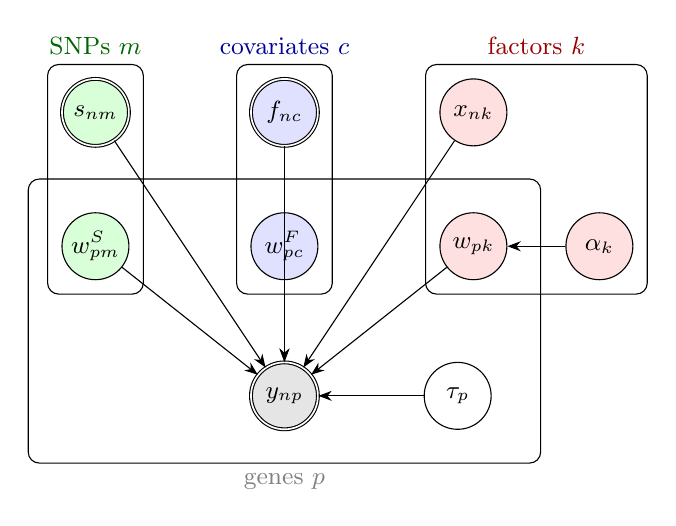
\begin{tikzpicture}[>=Stealth, every node/.style={font=\small},
      lat/.style={circle, draw, minimum size=0.85cm, inner sep=0pt},
      obs/.style={circle, draw, double, minimum size=0.85cm, inner sep=0pt},
      plate/.style={draw, rounded corners, inner sep=5pt}]
    \node[obs, fill=green!15] (s) at (0,2.6) {$s_{nm}$};
    \node[lat, fill=green!15] (ws) at (0,0.9) {$w^S_{pm}$};
    \node[obs, fill=blue!12] (f) at (2.4,2.6) {$f_{nc}$};
    \node[lat, fill=blue!12] (wf) at (2.4,0.9) {$w^F_{pc}$};
    \node[lat, fill=red!12] (x) at (4.8,2.6) {$x_{nk}$};
    \node[lat, fill=red!12] (w) at (4.8,0.9) {$w_{pk}$};
    \node[lat, fill=red!12] (al) at (6.4,0.9) {$\alpha_k$};
    \node[obs, fill=gray!20] (y) at (2.4,-1.0) {$y_{np}$};
    \node[lat] (tau) at (4.6,-1.0) {$\tau_p$};
    \draw[->] (s) -- (y); \draw[->] (ws) -- (y);
    \draw[->] (f) -- (y); \draw[->] (wf) -- (y);
    \draw[->] (x) -- (y); \draw[->] (w) -- (y);
    \draw[->] (al) -- (w); \draw[->] (tau) -- (y);
    \node[plate, fit=(s)(ws), label={[green!40!black]above:SNPs $m$}] {};
    \node[plate, fit=(f)(wf), label={[blue!60!black]above:covariates $c$}] {};
    \node[plate, fit=(x)(w)(al), label={[red!60!black]above:factors $k$}] {};
    \node[plate, fit=(ws)(wf)(w)(y)(tau), inner sep=12pt, label={[gray]below:genes $p$}] {};
  \end{tikzpicture}
  \caption{Graphical model of PEER, after \citet{stegle2010}. Double circles are observed; plates denote replication over SNPs, covariates, hidden factors and genes (the plate over individuals $n$, which contains $s_{nm}$, $f_{nc}$, $x_{nk}$ and $y_{np}$, is omitted for clarity). The ARD precision $\alpha_k$ controls whether hidden factor $k$ is used.}
  \label{fig:peer_model}
\end{figure}

\subsection{PEER in practice}

Fitting all four components of~\eqref{eq:peer} jointly is slow and difficult. In practice the genotype term is left out of the factor model: the known covariates and hidden factors are fitted first, as a pre-processing step, and the eQTL tests are then run with the simple regression~\eqref{eq:eqtl_lm}, either on the residuals or with the inferred factors $\hat\mX$ included as covariates. GTEx chose the number of PEER factors by sample size, using more factors for tissues with more samples. Simpler alternatives work about as well: taking the top principal components of the expression matrix as covariates, as in Chapter 8, matches or outperforms PEER in benchmarks~\citep{zhou2022pca}.

Removing hidden factors greatly increases the number of eQTLs found. In GTEx tissues, the number of eGenes detected at 5\% FDR roughly doubles as the number of PEER factors included as covariates increases from 0 to 60, with diminishing returns beyond that~\citep{fan2020}. Figure~\ref{fig:hidden_factors} shows the same effect on simulated data, which also shows ARD at work. The simulated expression of $P=2000$ genes in $N=200$ individuals has $K=10$ hidden factors and one cis SNP per gene, 30\% of which have a genetic effect. An ARD factor analysis model started with 30 factors keeps exactly 10 (Figure~\ref{fig:hidden_factors}a), and regressing out these factors finds as many eGenes as regressing out the true factors, three times as many as with no correction (Figure~\ref{fig:hidden_factors}b). Regressing out expression principal components improves power up to the true number of factors. Beyond that, extra components capture noise; removing them costs degrees of freedom and removes some genetic signal by chance, so power declines. In real data, with many confounders of decreasing strength, the curve usually rises and then plateaus instead.

\begin{figure}[!htbp]
  \centering
  \begin{subfigure}[b]{0.48\linewidth}
    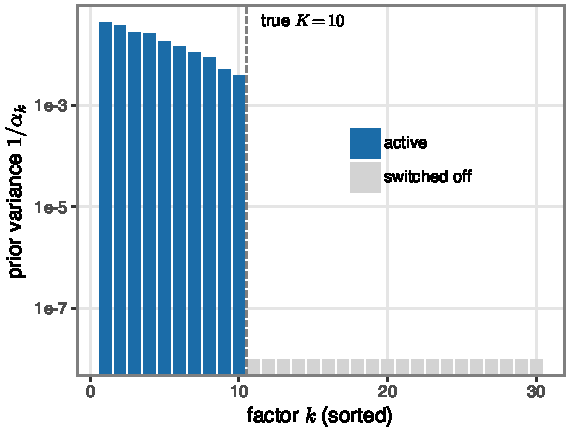
\includegraphics[width=\linewidth]{ard_factors.pdf}
    \caption{}
  \end{subfigure}\hfill
  \begin{subfigure}[b]{0.48\linewidth}
    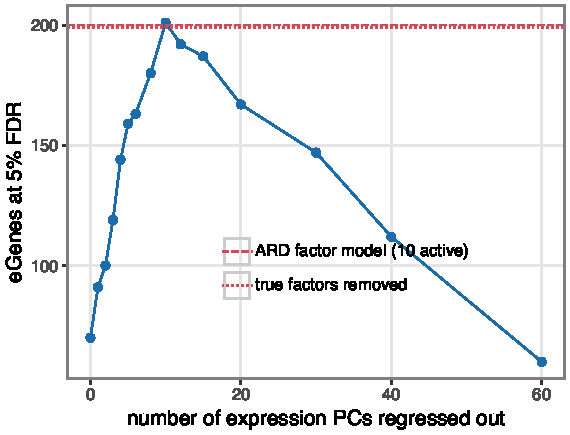
\includegraphics[width=\linewidth]{hidden_factors_power.pdf}
    \caption{}
  \end{subfigure}
  \caption{Removing hidden confounders from simulated expression ($N=200$ individuals, $P=2000$ genes, $K=10$ hidden factors). (a) Prior variances $1/\alpha_k$ of the factors of an ARD factor analysis model fitted with 30 factors (the switched-off factors are at the numerical floor $10^{-8}$). (b) eGenes detected at 5\% FDR after regressing out increasing numbers of expression principal components (blue), the 10 active ARD factors (dotted) or the true factors (dashed); the two horizontal lines coincide. The simulation has 617 true eGenes.}
  \label{fig:hidden_factors}
\end{figure}

There are two caveats. First, the factors should capture confounders, not the genetic signal itself. Cis effects are specific to one gene each and are not low-rank, so they survive. A trans-acting variant that changes the expression of many genes, for example through a transcription factor, does produce low-rank structure, and regressing out factors can remove it; hidden-factor correction is therefore risky for trans-eQTL analysis. Second, factors can capture interesting biology, such as cell type composition or an immune response. Removing them helps in finding eQTLs that act in all conditions, at the cost of hiding those whose effect depends on the condition (Section~\ref{sec:interaction}).

%======================================================================
\section{Cis and trans effects}
%======================================================================

A cis-eQTL acts on the copy of the gene on the same chromosome, typically through a promoter or enhancer variant that changes transcription factor binding (Figure~\ref{fig:cis_trans}, top). Cis-eQTLs are the classical eQTL: they are robust, replicate well between studies, and can be found with as few as 70 individuals. A \emph{trans}-eQTL acts at a distance, usually on another chromosome. A typical mechanism is a variant that changes the expression or the protein sequence of a transcription factor, which then changes the expression of the factor's targets throughout the genome (Figure~\ref{fig:cis_trans}, bottom). Trans effects are biologically interesting, since they reveal regulatory networks, but they are hard to find and to replicate. Each effect is small, and without a window to restrict the search we are back to testing millions of SNPs per gene, with a testing burden of millions of SNPs times $20{,}000$ genes. Reliable trans-eQTL mapping needs thousands of individuals, and false positives from technical artefacts, such as reads from one gene mis-mapped to a paralogous gene elsewhere in the genome, are a constant worry.

The cis-trans distinction is about mechanism, not distance alone: a cis effect is one that acts only on the allele on the same DNA molecule. This is what allele-specific expression measures, as we see next. In practice, eQTL studies use physical distance as a proxy and call any SNP within 1\,Mb of a gene cis.

\begin{figure}[!htbp]
  \centering
  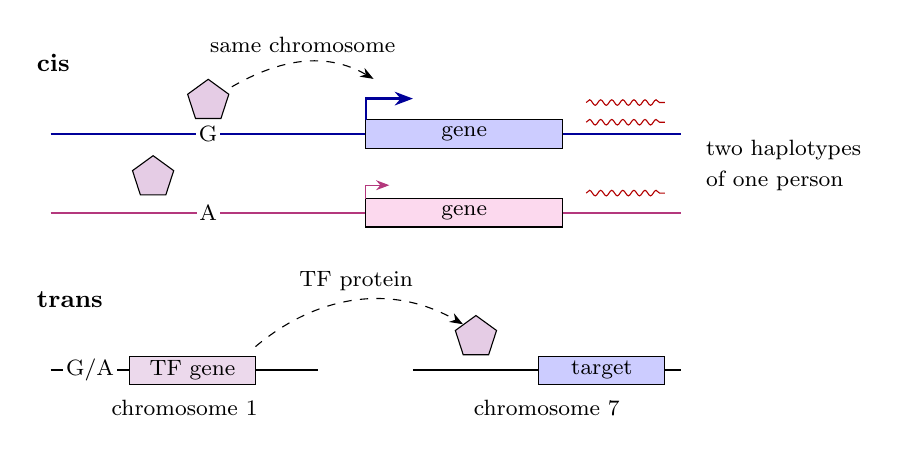
\begin{tikzpicture}[>=Stealth, every node/.style={font=\small}, tf/.style={regular polygon, regular polygon sides=5, draw, fill=violet!20, minimum size=0.55cm, inner sep=0pt}]
    % cis
    \node[anchor=west] at (-0.3,0.9) {\textbf{cis}};
    \draw[thick, blue!60!black] (0,0) -- (8,0);
    \draw[fill=blue!20] (4,-0.18) rectangle (6.5,0.18);
    \node at (5.25,0) {\footnotesize gene};
    \draw[->, thick, blue!60!black] (4,0.18) -- (4,0.45) -- (4.6,0.45);
    \node[tf] at (2,0.42) {};
    \node[fill=white, inner sep=1pt] at (2,0) {\footnotesize G};
    \draw[->, dashed] (2.3,0.6) to[out=30, in=150] node[above] {\footnotesize same chromosome} (4.1,0.7);
    \draw[thick, magenta!70!black] (0,-1.0) -- (8,-1.0);
    \draw[fill=magenta!15] (4,-1.18) rectangle (6.5,-0.82);
    \node at (5.25,-1.0) {\footnotesize gene};
    \draw[->, magenta!70!black] (4,-0.82) -- (4,-0.65) -- (4.3,-0.65);
    \node[fill=white, inner sep=1pt] at (2,-1.0) {\footnotesize A};
    \node[tf] at (1.3,-0.55) {};
    \draw[decorate, decoration={snake, amplitude=1pt, segment length=4pt}, red!70!black] (6.8,0.15) -- (7.8,0.15);
    \draw[decorate, decoration={snake, amplitude=1pt, segment length=4pt}, red!70!black] (6.8,0.40) -- (7.8,0.40);
    \draw[decorate, decoration={snake, amplitude=1pt, segment length=4pt}, red!70!black] (6.8,-0.75) -- (7.8,-0.75);
    \node[right, align=left] at (8.2,-0.4) {\footnotesize two haplotypes\\\footnotesize of one person};
    % trans
    \begin{scope}[yshift=-3.0cm]
      \node[anchor=west] at (-0.3,0.9) {\textbf{trans}};
      \draw[thick] (0,0) -- (3.4,0);
      \draw[fill=violet!15] (1.0,-0.18) rectangle (2.6,0.18);
      \node at (1.8,0) {\footnotesize TF gene};
      \node[fill=white, inner sep=1pt] at (0.5,0) {\footnotesize G/A};
      \node[below] at (1.7,-0.25) {\footnotesize chromosome 1};
      \draw[thick] (4.6,0) -- (8,0);
      \draw[fill=blue!20] (6.2,-0.18) rectangle (7.8,0.18);
      \node at (7.0,0) {\footnotesize target};
      \node[below] at (6.3,-0.25) {\footnotesize chromosome 7};
      \node[tf] (t) at (5.4,0.42) {};
      \draw[->, dashed] (2.6,0.3) to[out=40, in=150] node[above] {\footnotesize TF protein} (t.north west);
    \end{scope}
  \end{tikzpicture}
  \caption{Cis and trans effects. Top: a cis-regulatory variant changes binding of a transcription factor (pentagon) near a gene and so changes expression only of the copy of the gene on the same chromosome, giving more RNA from the G haplotype. Bottom: a trans effect, in which a variant in or near a transcription factor (TF) gene changes the TF's level or activity, which changes expression of its target genes elsewhere in the genome, on both of their copies.}
  \label{fig:cis_trans}
\end{figure}

%======================================================================
\section{Linkage disequilibrium and the causal variant}
%======================================================================

An eQTL association has the same problem as a GWAS association: LD. Figure~\ref{fig:ld_locus} shows a simulated cis window in which one SNP affects expression. Many SNPs in high LD with it are almost as significant, SNPs in moderate LD are moderately significant, and with a little noise the most significant SNP need not be the causal one. SNPs in LD act as proxies, or \emph{tag SNPs}, for the causal variant. The ease of finding an associated locus and the difficulty of finding the variant within it are two sides of the same coin. Fine-mapping methods (Chapter 11), such as SuSiE~\citep{wang2020susie}, compute for each SNP the posterior probability that it is causal and report credible sets that contain a causal variant with high probability, allowing for several causal variants per gene. Functional annotations can sharpen the posterior (Section~\ref{sec:annotations}). The definitive test is experimental: editing the variant with CRISPR and measuring expression, which has been done for the lead variants of some eQTLs.

\begin{figure}[!htbp]
  \centering
  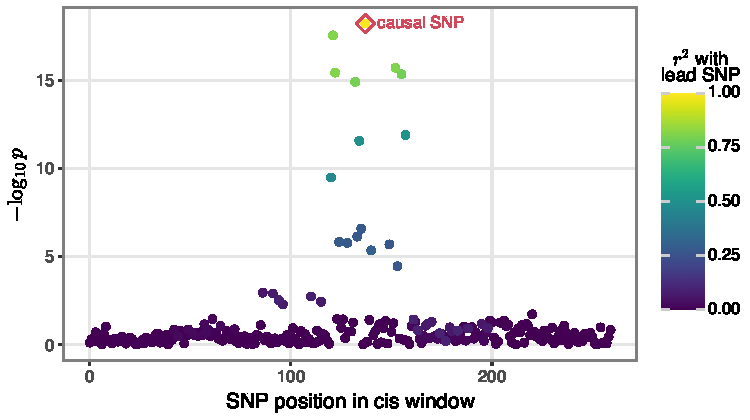
\includegraphics[width=0.7\linewidth]{ld_locus.pdf}
  \caption{A simulated cis-eQTL with one causal SNP (diamond) among 260 SNPs with block-like LD, in $N=500$ individuals. Each point is a SNP, coloured by its LD ($r^2$) with the most significant (lead) SNP. SNPs in high LD with the causal variant are nearly as significant as the causal variant.}
  \label{fig:ld_locus}
\end{figure}

%======================================================================
\section{Allele-specific expression}
\label{sec:ase}
%======================================================================

\subsection{Two views of the same cis effect}

A cis-eQTL can be seen in two ways (Figure~\ref{fig:ase}). Across individuals, those with more copies of the high-expression allele have higher total expression of the gene. Within a single individual who is heterozygous at the regulatory variant, the copy of the gene on the haplotype with the high-expression allele produces more RNA than the copy on the other haplotype. (A \emph{haplotype} is the sequence of one of the two copies of a chromosome, one inherited from each parent.) To see the within-individual difference we need a way to tell the RNA from the two copies apart. If the individual is also heterozygous at a SNP in the transcribed sequence, for example a coding or UTR SNP with alleles T and C, RNA-seq reads that cover it carry one allele or the other, and counting them measures \emph{allele-specific expression} (ASE). An imbalance away from 50:50 indicates a cis-regulatory difference between the two haplotypes.

\begin{figure}[!htbp]
  \centering
  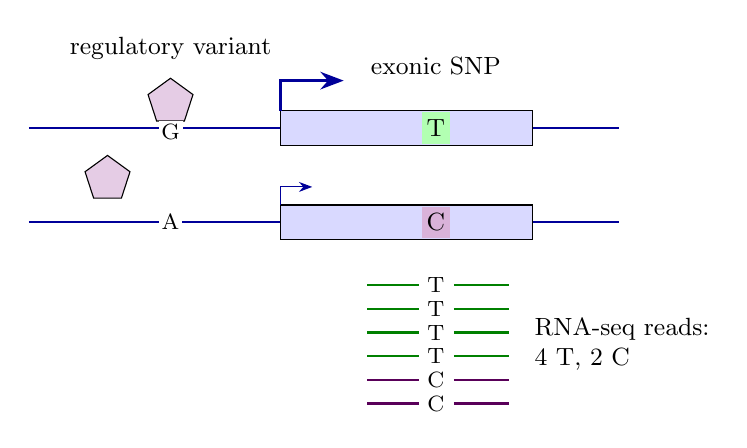
\begin{tikzpicture}[>=Stealth, every node/.style={font=\small}, tf/.style={regular polygon, regular polygon sides=5, draw, fill=violet!20, minimum size=0.6cm, inner sep=0pt}]
    \draw[thick, blue!60!black] (0,0) -- (7.5,0);
    \draw[fill=blue!15] (3.2,-0.22) rectangle (6.4,0.22);
    \fill[green!30] (5.0,-0.2) rectangle (5.35,0.2); \node at (5.17,0) {T};
    \draw[->, very thick, blue!60!black] (3.2,0.22) -- (3.2,0.6) -- (4.0,0.6);
    \node[tf] at (1.8,0.33) {};
    \node[fill=white, inner sep=1pt] at (1.8,-0.05) {\footnotesize G};
    \draw[thick, blue!60!black] (0,-1.2) -- (7.5,-1.2);
    \draw[fill=blue!15] (3.2,-1.42) rectangle (6.4,-0.98);
    \fill[violet!30] (5.0,-1.4) rectangle (5.35,-1.0); \node at (5.17,-1.2) {C};
    \draw[->, blue!60!black] (3.2,-0.98) -- (3.2,-0.75) -- (3.6,-0.75);
    \node[fill=white, inner sep=1pt] at (1.8,-1.2) {\footnotesize A};
    \node[tf] at (1.0,-0.65) {};
    \node[above] at (1.8,0.75) {regulatory variant};
    \node[above] at (5.17,0.55) {exonic SNP};
    % reads
    \foreach \y/\a in {-2.0/T,-2.3/T,-2.6/T,-2.9/T} {
      \draw[green!50!black, thick] (4.3,\y) -- (4.95,\y); \draw[green!50!black, thick] (5.4,\y) -- (6.1,\y);
      \node at (5.17,\y) {\footnotesize \a};}
    \foreach \y/\a in {-3.2/C,-3.5/C} {
      \draw[violet!70!black, thick] (4.3,\y) -- (4.95,\y); \draw[violet!70!black, thick] (5.4,\y) -- (6.1,\y);
      \node at (5.17,\y) {\footnotesize \a};}
    \node[right, align=left] at (6.3,-2.75) {RNA-seq reads:\\4 T, 2 C};
  \end{tikzpicture}
  \caption{Allele-specific expression. In an individual heterozygous at a regulatory variant, a transcription factor (pentagon) binds the G allele but not the A allele, so the copy of the gene on the G haplotype is expressed more. If the individual is also heterozygous at a SNP in the transcript (T/C), RNA-seq reads covering it can be assigned to a haplotype, and the read counts show the imbalance.}
  \label{fig:ase}
\end{figure}

ASE requires an individual to be heterozygous at a transcribed SNP, and, to connect the imbalance to a candidate regulatory variant, the phase of the two SNPs: which allele of the regulatory variant lies on the same haplotype as which allele of the exonic SNP. Phase is estimated statistically from population genotype data or read directly from long reads. The heterozygous exonic SNP is only a marker. It is usually not the cause of the imbalance, which is due to some other variant in cis. The same idea applies to other sequencing assays. In ChIP-seq or ATAC-seq, reads overlapping a heterozygous SNP in a binding site or accessible region measure allele-specific binding or accessibility, and there the SNP being counted is often itself the cause, since a variant inside a binding site can directly change binding.

\subsection{Counting alleles: binomial and beta-binomial models}

Consider one individual and one heterozygous exonic SNP. Let $d$ be the number of reads covering the SNP that carry either allele, $y\leq d$ the number carrying the reference allele, and $\pi$ the expected fraction of reads from the reference haplotype. If reads were independent draws,
\begin{equation}
  y\mid d,\pi \sim \Bin(d,\pi), \qquad \Pr(y\mid d,\pi) = \binom{d}{y}\pi^y(1-\pi)^{d-y},
\end{equation}
and testing for allelic imbalance means testing $H_0:\pi=1/2$. Reads are not independent draws, however. Library preparation amplifies the cDNA by PCR, so several reads can come from one original molecule; mapping and capture efficiencies vary from site to site; and the true imbalance varies between individuals and cells. All of these make the counts more variable than the binomial allows, and a binomial test applied to such data reports far too many significant imbalances.

The \emph{beta-binomial} distribution adds this extra variation by treating $\pi$ as random. Let $\pi\sim\BetaDist(a,b)$ with $a,b>0$ and density
\begin{equation}
  p(\pi\mid a,b) = \frac{\pi^{a-1}(1-\pi)^{b-1}}{\BetaFn(a,b)}, \qquad \BetaFn(a,b)=\int_0^1 u^{a-1}(1-u)^{b-1}du = \frac{\Gamma(a)\Gamma(b)}{\Gamma(a+b)}.
\end{equation}
The beta is the conjugate prior of the binomial (the density has the same form $\pi^{\cdot}(1-\pi)^{\cdot}$ as the likelihood) and is the two-category case of the Dirichlet distribution used for isoform proportions in Chapter 10. Its mean and variance are
\begin{equation}
  \E[\pi] = \frac{a}{a+b}=:\mu, \qquad \Var(\pi) = \frac{ab}{(a+b)^2(a+b+1)} = \frac{\mu(1-\mu)}{c+1},
\end{equation}
where $c=a+b$ is the \emph{concentration}. The ratio of $a$ to $b$ sets the mean, and the concentration sets how tightly $\pi$ is distributed around it. Integrating $\pi$ out gives the beta-binomial,
\begin{align}
  \Pr(y\mid d,a,b) &= \int_0^1\binom{d}{y}\pi^y(1-\pi)^{d-y}\,\frac{\pi^{a-1}(1-\pi)^{b-1}}{\BetaFn(a,b)}\,d\pi \nonumber\\
  &= \binom{d}{y}\frac{1}{\BetaFn(a,b)}\int_0^1\pi^{y+a-1}(1-\pi)^{d-y+b-1}\,d\pi
  = \binom{d}{y}\frac{\BetaFn(y+a,\,d-y+b)}{\BetaFn(a,b)}.
  \label{eq:betabinom}
\end{align}
We write $\BetaBin(y\mid d,\mu,c)$ for this distribution parameterized by its mean fraction $\mu=a/c$ and concentration $c$, so $a=\mu c$ and $b=(1-\mu)c$. The moments follow from the laws of total expectation and variance. The mean is $\E[y]=\E[\E[y\mid\pi]]=d\E[\pi]=d\mu$. For the variance,
\begin{align}
  \Var(y) &= \E[\Var(y\mid\pi)] + \Var(\E[y\mid\pi]) = d\,\E[\pi(1-\pi)] + d^2\Var(\pi) \nonumber\\
  &= d\big(\mu(1-\mu)-\Var(\pi)\big) + d^2\Var(\pi) = d\mu(1-\mu) + d(d-1)\Var(\pi) \nonumber\\
  &= d\mu(1-\mu)\left[1+\frac{d-1}{c+1}\right],
\end{align}
using $\E[\pi(1-\pi)]=\E[\pi]-\E[\pi^2]=\mu-\Var(\pi)-\mu^2$. The first factor is the binomial variance, and the bracket is the overdispersion factor. As $c\to\infty$ it tends to one and the beta-binomial becomes the binomial; small $c$ means noisy allelic counts. Figure~\ref{fig:count_models}a compares a binomial and a beta-binomial with the same mean: the beta-binomial with $c=17$ and $d=30$ has a variance $2.6$ times larger.

\subsection{Counting molecules: Poisson and negative binomial models}

The total read count for a gene in an individual is a count without a fixed number of trials. The basic model is the Poisson, $y\sim\Pois(\lambda)$ with $\Pr(y\mid\lambda)=\lambda^ye^{-\lambda}/y!$, the limit of a binomial with many trials, each with small success probability. Like the binomial it has one parameter: $\E[y]=\Var(y)=\lambda$, so fixing the mean fixes the variance. RNA-seq counts are much more variable between biological replicates than this, for the same reasons as allelic counts and because true expression varies between individuals.

The fix follows the same recipe. Let the rate be random, $\lambda\sim\Gam(\phi,r)$ with shape $\phi$ and rate $r$, density $r^\phi\lambda^{\phi-1}e^{-r\lambda}/\Gamma(\phi)$, mean $\phi/r$ and variance $\phi/r^2$. The gamma is conjugate to the Poisson, and integrating out $\lambda$ gives
\begin{align}
  \Pr(y\mid\phi,r) &= \int_0^\infty \frac{\lambda^ye^{-\lambda}}{y!}\,\frac{r^\phi\lambda^{\phi-1}e^{-r\lambda}}{\Gamma(\phi)}\,d\lambda
  = \frac{r^\phi}{y!\,\Gamma(\phi)}\int_0^\infty\lambda^{y+\phi-1}e^{-(r+1)\lambda}\,d\lambda \nonumber\\
  &= \frac{r^\phi}{y!\,\Gamma(\phi)}\,\frac{\Gamma(y+\phi)}{(r+1)^{y+\phi}}
  = \frac{\Gamma(y+\phi)}{\Gamma(\phi)\,y!}\left(\frac{r}{r+1}\right)^\phi\left(\frac{1}{r+1}\right)^y,
\end{align}
the \emph{negative binomial} distribution, better described as the gamma-Poisson. (Its name comes from another derivation, as the number of failures before the $\phi$-th success in a sequence of coin flips with success probability $r/(r+1)$.) The mean is $m=\E[y]=\E[\lambda]=\phi/r$, and by the law of total variance
\begin{equation}
  \Var(y) = \E[\Var(y\mid\lambda)]+\Var(\E[y\mid\lambda]) = \E[\lambda]+\Var(\lambda) = \frac{\phi}{r}+\frac{\phi}{r^2} = m + \frac{m^2}{\phi}.
\end{equation}
We write $\NB(y\mid m,\phi)$ for the distribution with mean $m$ and shape $\phi$, so $r=\phi/m$. The variance always exceeds the Poisson variance $m$, by an amount controlled by the shape, which plays the role of a concentration: as $\phi\to\infty$ we recover the Poisson. $1/\phi$ is called the dispersion, and the same model underlies standard differential expression tools. Figure~\ref{fig:count_models}b compares a Poisson and a negative binomial with mean 30; with $\phi=8$ the variance is $30+900/8=142.5$ rather than 30.

\begin{figure}[!htbp]
  \centering
  \begin{subfigure}[b]{0.48\linewidth}
    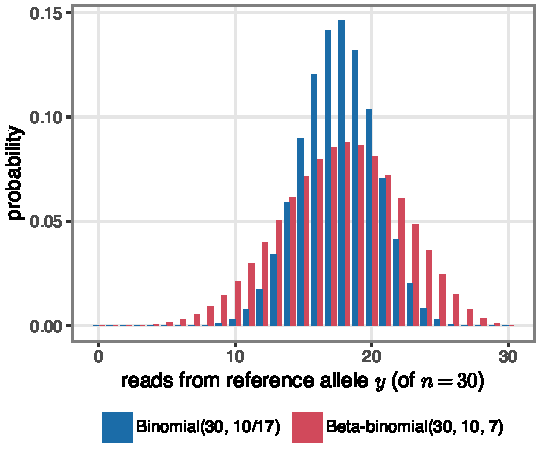
\includegraphics[width=\linewidth]{betabinom.pdf}
    \caption{}
  \end{subfigure}\hfill
  \begin{subfigure}[b]{0.48\linewidth}
    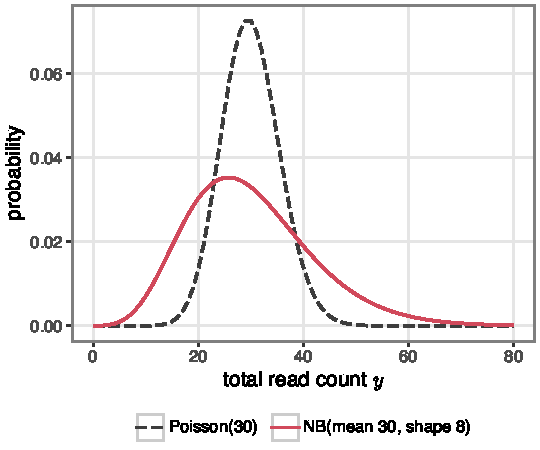
\includegraphics[width=\linewidth]{negbin.pdf}
    \caption{}
  \end{subfigure}
  \caption{Overdispersed count models. (a) Binomial with $d=30$ trials and $\pi=10/17$ and beta-binomial with $d=30$, $a=10$, $b=7$; both have mean 17.6, but the variances are 7.3 and 19.0. (b) Poisson with mean 30 and negative binomial with mean 30 and shape $\phi=8$.}
  \label{fig:count_models}
\end{figure}

\subsection{Combining total and allele-specific counts}

The combined haplotype test (CHT)~\citep{mcvicker2013}, implemented in WASP~\citep{vandegeijn2015}, uses both the between-individual signal in total counts and the within-individual signal in allelic counts to test a candidate cis-regulatory SNP. We describe a simplified version. Let $\theta_R$ and $\theta_A$ be the expression of one copy of the gene on a haplotype carrying the reference and the alternative allele of the test SNP. The expected allelic fraction in a heterozygote is the \emph{allelic imbalance}
\begin{equation}
  \pi = \frac{\theta_R}{\theta_R+\theta_A},
\end{equation}
and the expected total expression of individual $n$ depends on their genotype at the test SNP,
\begin{equation}
  \lambda_n = T_n\times\begin{cases} 2\theta_R & \text{if $n$ is homozygous reference},\\ \theta_R+\theta_A & \text{if $n$ is heterozygous},\\ 2\theta_A & \text{if $n$ is homozygous alternative}, \end{cases}
\end{equation}
where $T_n$ is a scaling factor for how deeply individual $n$ was sequenced. This is the additive model of~\eqref{eq:eqtl_lm} on the count scale. For individual $n$, let $y^t_n$ be the total read count of the gene and $y^a_n$ the number of reads from the haplotype carrying the reference allele of the test SNP, out of $d_n$ reads covering heterozygous exonic SNPs (using the phase to assign reads to haplotypes). The likelihood is
\begin{equation}
  L(\theta_R,\theta_A) = \prod_{n=1}^N \NB\big(y^t_n\mid\lambda_n,\phi\big)\;\prod_{n:\,\text{het}}\BetaBin\big(y^a_n\mid d_n,\pi,c\big)\;\prod_{n:\,\text{hom}}\BetaBin\big(y^a_n\mid d_n,\tfrac12,c\big),
  \label{eq:cht}
\end{equation}
with shape $\phi$ and concentration $c$ estimated across genes. Individuals who are homozygous at the test SNP have the same regulatory allele on both haplotypes, so their allelic counts are expected to be balanced; their term does not depend on $\theta$, but it would show imbalance, and so evidence against this SNP, if the true causal variant were a different one. The test of $H_0:\theta_R=\theta_A$ is a \emph{likelihood ratio test}: maximize~\eqref{eq:cht} with $\theta_R$ and $\theta_A$ free and with $\theta_R=\theta_A$, and compare
\begin{equation}
  \Lambda = 2\left[\log L(\hat\theta_R,\hat\theta_A) - \log L(\hat\theta_0,\hat\theta_0)\right]
\end{equation}
with a $\chi^2_1$ distribution, which by Wilks' theorem is its distribution under the null for large samples. The full CHT also models genotyping errors and estimates the dispersions per individual. WASP also corrects \emph{reference mapping bias}: reads carrying the reference allele align to the reference genome slightly more easily than reads carrying the alternative allele, which mimics allelic imbalance. WASP flips the allele in each read that overlaps a SNP, remaps it, and discards reads that do not map to the same place. RASQUAL~\citep{kumasaka2016} is a related model that combines the two signals and also handles uncertainty in phasing.

\subsection{Calibration and power}

Results of genome-wide tests are summarized by \emph{quantile-quantile (QQ) plots} (Figure~\ref{fig:ase_qq}). If the test is calibrated, its p values are uniform on $[0,1]$ under the null. We sort the $J$ observed p values and plot $-\log_{10}$ of each against $-\log_{10}$ of the corresponding uniform quantile, $(i-0.5)/J$ for the $i$-th smallest. If there is no signal, the points lie on the diagonal. True associations bend the curve upward at the right, while a curve that leaves the diagonal from the start indicates a miscalibrated test or confounding.

Figure~\ref{fig:ase_qq} shows both effects on simulated data with 20 individuals and 2000 SNP-gene pairs, 20\% with a true cis effect, using overdispersed counts ($\phi=10$, $c=30$). On null genes (panel a), a binomial test of allelic imbalance is badly inflated: 14\% of null tests have $p<0.05$. The beta-binomial test with the correct concentration is calibrated (5.4\%). On all genes (panel b), the combined test of~\eqref{eq:cht} finds more than twice as many associations at 5\% FDR as a linear regression on log total counts (232 versus 95 of 407 true effects). \citet{vandegeijn2015} found the same in real data: on H3K27ac ChIP-seq from only 10 lymphoblastoid cell lines, where the linear model found almost nothing, the combined test found many histone QTLs, and it also found substantially more eQTLs in 70 lymphoblastoid cell lines.

\begin{figure}[!htbp]
  \centering
  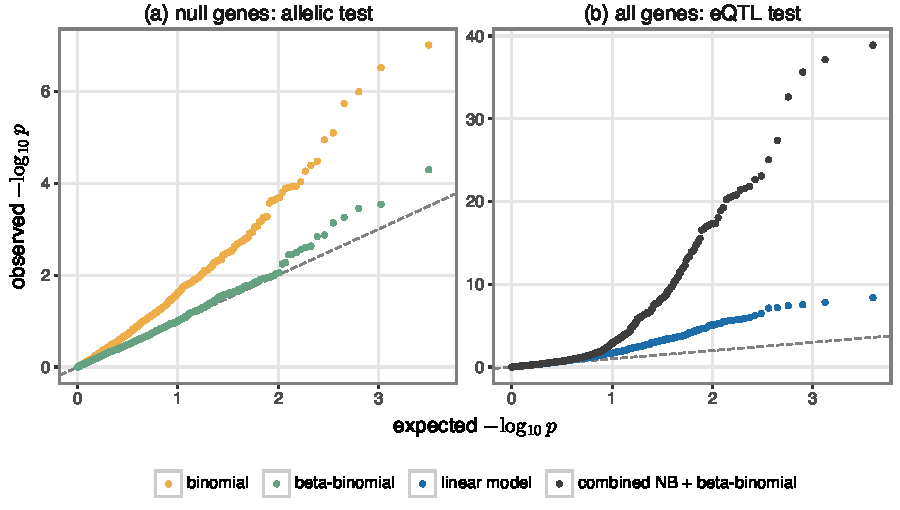
\includegraphics[width=0.9\linewidth]{ase_qq.pdf}
  \caption{QQ plots of simulated allele-specific tests ($N=20$ individuals, 2000 SNP-gene pairs, 20\% with a cis effect, overdispersed counts). (a) Tests of allelic imbalance among heterozygotes on null genes: the binomial test is inflated, the beta-binomial test is calibrated. (b) eQTL tests on all genes: linear regression of log total counts on genotype, and the combined likelihood ratio test of total (negative binomial) and allelic (beta-binomial) counts. Dashed line, $y=x$.}
  \label{fig:ase_qq}
\end{figure}

Why is the within-individual comparison so powerful? The two haplotypes of an individual are in the same cells, in the same tissue, exposed to the same environment and processed in the same experiment. Comparing them is a built-in control: almost all of the technical and environmental variation that differs between people cancels, leaving the effect of the sequence difference. This gives some insight into regulatory variation even with very small samples, where between-individual eQTL mapping fails. It also separates cis from trans effects, since a trans effect, acting through a diffusible factor, affects both copies of a gene equally. The limitations are that a gene must carry a heterozygous transcribed SNP with enough reads in enough individuals, and that the extra machinery (phasing, mapping bias correction, overdispersion) makes the analysis slower and more involved.

%======================================================================
\section{Lessons from tissue atlases}
%======================================================================

\subsection{eQTLs and sQTLs across tissues}

The Genotype-Tissue Expression (GTEx) project collected RNA-seq from around 50 tissues of almost 1000 post-mortem donors, with whole-genome sequencing of each donor~\citep{gtex2017,gtex2020}. The number of samples per tissue ranges from under 100 to around 700, because some tissues are much harder to collect than others. Figure~\ref{fig:gtex_egenes} shows the fraction of tested genes with a significant cis-eQTL or cis-sQTL in each tissue. Discovery grows steadily with sample size and has not saturated, and eQTLs are easier to detect than sQTLs. Across tissues, 95\% of protein-coding genes have at least one cis-eQTL and 79\% at least one cis-sQTL. With larger samples, conditional analysis (adding the lead variant as a covariate and searching again) finds a second, third or further independent eVariant for an increasing fraction of genes, so the one-causal-variant-per-gene picture is a consequence of limited power rather than biology. Trans-eQTLs were found for only on the order of a hundred genes, consistent with their small effects.

\begin{figure}[!htbp]
  \centering
  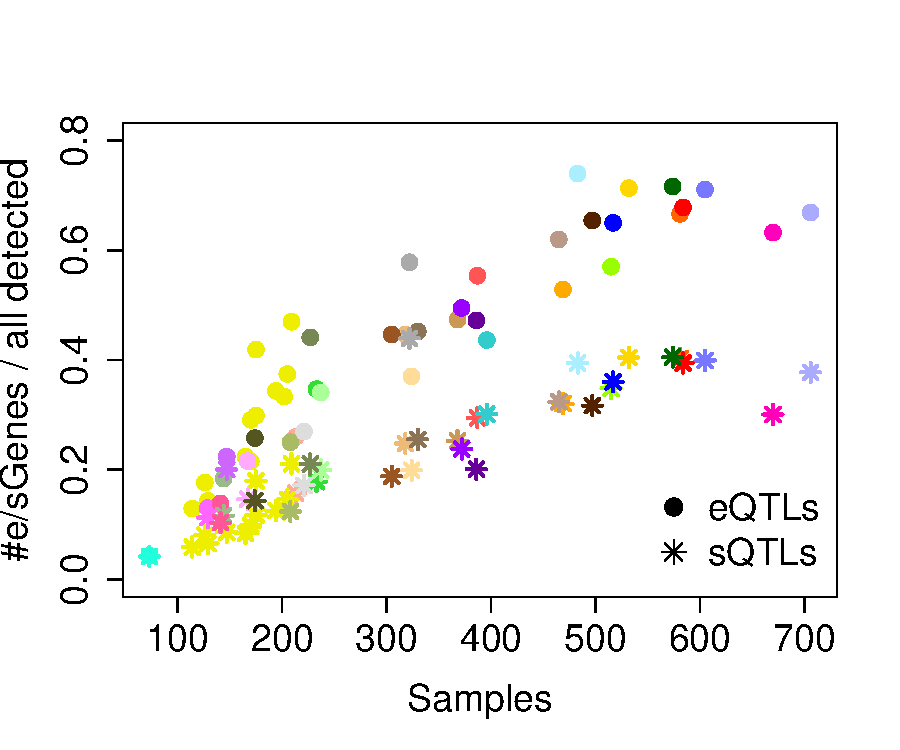
\includegraphics[width=0.5\linewidth]{slides/gtex_egenes.pdf}
  \caption{Fraction of tested genes with a cis-eQTL (eGenes, dots) or cis-sQTL (sGenes, stars) at 5\% FDR, against the number of samples, for each GTEx tissue (colours). From the GTEx Consortium~\citep{gtex2020}.}
  \label{fig:gtex_egenes}
\end{figure}

\subsection{Sharing of eQTLs across tissues}

How much of the genetic regulation of expression is shared between tissues? The naive approach maps eQTLs separately in each tissue and counts how often an eQTL significant in one is also significant in another. This confuses the absence of evidence with evidence of absence. Tissues differ in sample size and therefore in power, so an eQTL can be significant in one tissue and not another just because the second has fewer samples. Figure~\ref{fig:sharing_naive} shows this for simulated eQTLs whose true effects are identical in two tissues with 500 and 150 samples: of the eQTLs significant in at least one tissue, 77\% are significant only in the larger one and would be called tissue-specific. Early studies made exactly this mistake and concluded that eQTLs are mostly tissue-specific. The general lesson is that comparing ``significant in condition 1'' with ``significant in condition 2'' is not a test of whether the effect differs; that requires a model of the effects in both conditions together.

\begin{figure}[!htbp]
  \centering
  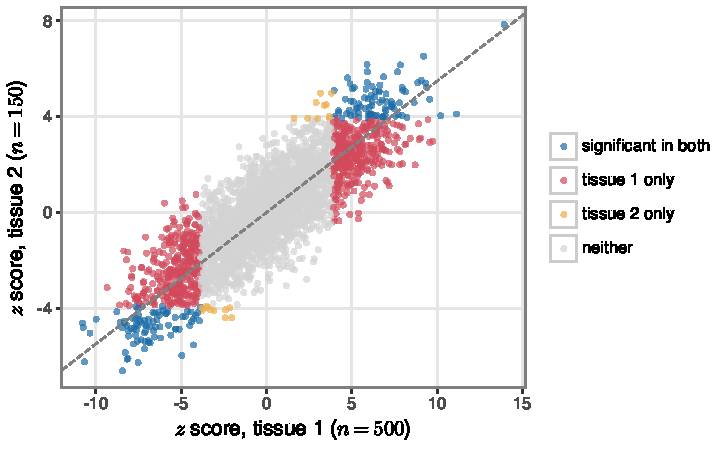
\includegraphics[width=0.62\linewidth]{sharing_naive.pdf}
  \caption{The ``significant here, not there'' fallacy. Simulated $z$ scores for 3000 eQTLs with the same true effect in two tissues, measured in 500 and 150 individuals. Points are coloured by whether they pass $p<10^{-4}$ in both, one or neither tissue. Most eQTLs significant in the larger tissue are not significant in the smaller one, although none is tissue-specific. Dashed line, the expected ratio $\sqrt{150/500}$ of the $z$ scores.}
  \label{fig:sharing_naive}
\end{figure}

Multivariate adaptive shrinkage (mash)~\citep{urbut2019} models the effects jointly from summary statistics. For SNP-gene pair $j$ and tissue $r=1,\dots,R$, let $b_{jr}$ be the true effect, $\hat b_{jr}$ its estimate (from~\eqref{eq:eqtl_lm} or another test) and $s_{jr}$ the standard error of $\hat b_{jr}$. Collect them into vectors $\vbb_j,\vbhat_j\in\R^R$ and the diagonal matrix $\mS_j=\diag(s_{j1}^2,\dots,s_{jR}^2)$. The likelihood treats the estimates as unbiased and normally distributed,
\begin{equation}
  \vbhat_j\mid\vbb_j \sim \Normal(\vbb_j,\mS_j),
\end{equation}
which can be extended to correlated errors when tissues share donors. The prior on the vector of true effects is a mixture of zero-mean multivariate normals,
\begin{equation}
  \vbb_j \sim \sum_{k=1}^K\sum_{l=1}^L \pi_{kl}\,\Normal(\vzero,\omega_l\mU_k), \qquad \sum_{k,l}\pi_{kl}=1,
  \label{eq:mash_prior}
\end{equation}
where each $\mU_k\in\R^{R\times R}$ is a candidate covariance matrix describing a pattern of sharing across tissues, $\omega_l>0$ is one of $L$ scaling factors on a fixed grid, and $\pi_{kl}\geq0$ are mixture weights. The $\mU_k$ include \emph{canonical} matrices (the identity, for independent effects in each tissue; a matrix of ones, for an identical effect in all tissues; and $R$ matrices with a single non-zero diagonal entry, for an effect in only one tissue) and \emph{data-driven} matrices estimated from the strongest associations, for example by PCA or sparse factor analysis of their $z$ scores. Because the prior and likelihood are Gaussian, $\vbb_j$ can be integrated out within each component,
\begin{equation}
  \vbhat_j \sim \sum_{k,l}\pi_{kl}\,\Normal\big(\vzero,\ \omega_l\mU_k+\mS_j\big),
\end{equation}
and only the weights $\pi_{kl}$ are learned, by maximizing this likelihood over many SNP-gene pairs. The problem is convex in $\pi$ and is solved by EM or convex optimization. With the weights fixed, Bayes' rule gives a posterior for each $\vbb_j$ that is again a mixture of normals. For component $(k,l)$ with prior covariance $\mSigma_{kl}=\omega_l\mU_k$, the posterior covariance and mean are
\begin{equation}
  \mV_{jkl} = \big(\mSigma_{kl}^{-1}+\mS_j^{-1}\big)^{-1}, \qquad \vm_{jkl} = \mV_{jkl}\mS_j^{-1}\vbhat_j,
\end{equation}
and the posterior component weights are $\tilde\pi_{jkl}\propto\pi_{kl}\Normal(\vbhat_j;\vzero,\mSigma_{kl}+\mS_j)$. The posterior means shrink noisy estimates toward the sharing patterns that are common in the data, borrowing strength across tissues. Sharing is then assessed on the posterior effects, for example by asking in which tissues the posterior mean has the same sign as, and is within a factor of two of, the strongest effect, and significance by the \emph{local false sign rate} (lfsr), the posterior probability that the sign of the effect is wrong.

Applied to GTEx, mash estimated that the effects of cis-eQTLs are strongly correlated across tissues (Figure~\ref{fig:mash_heatmap}). The brain regions form a highly correlated block, as do related tissues such as the two skin samples, the arteries and the parts of the gut, while testis, liver, whole blood and lymphoblastoid cells are the most distinct. From an expression genetics point of view the many brain regions sampled by GTEx look much alike; more donors would have given more information than more regions.

\begin{figure}[!htbp]
  \centering
  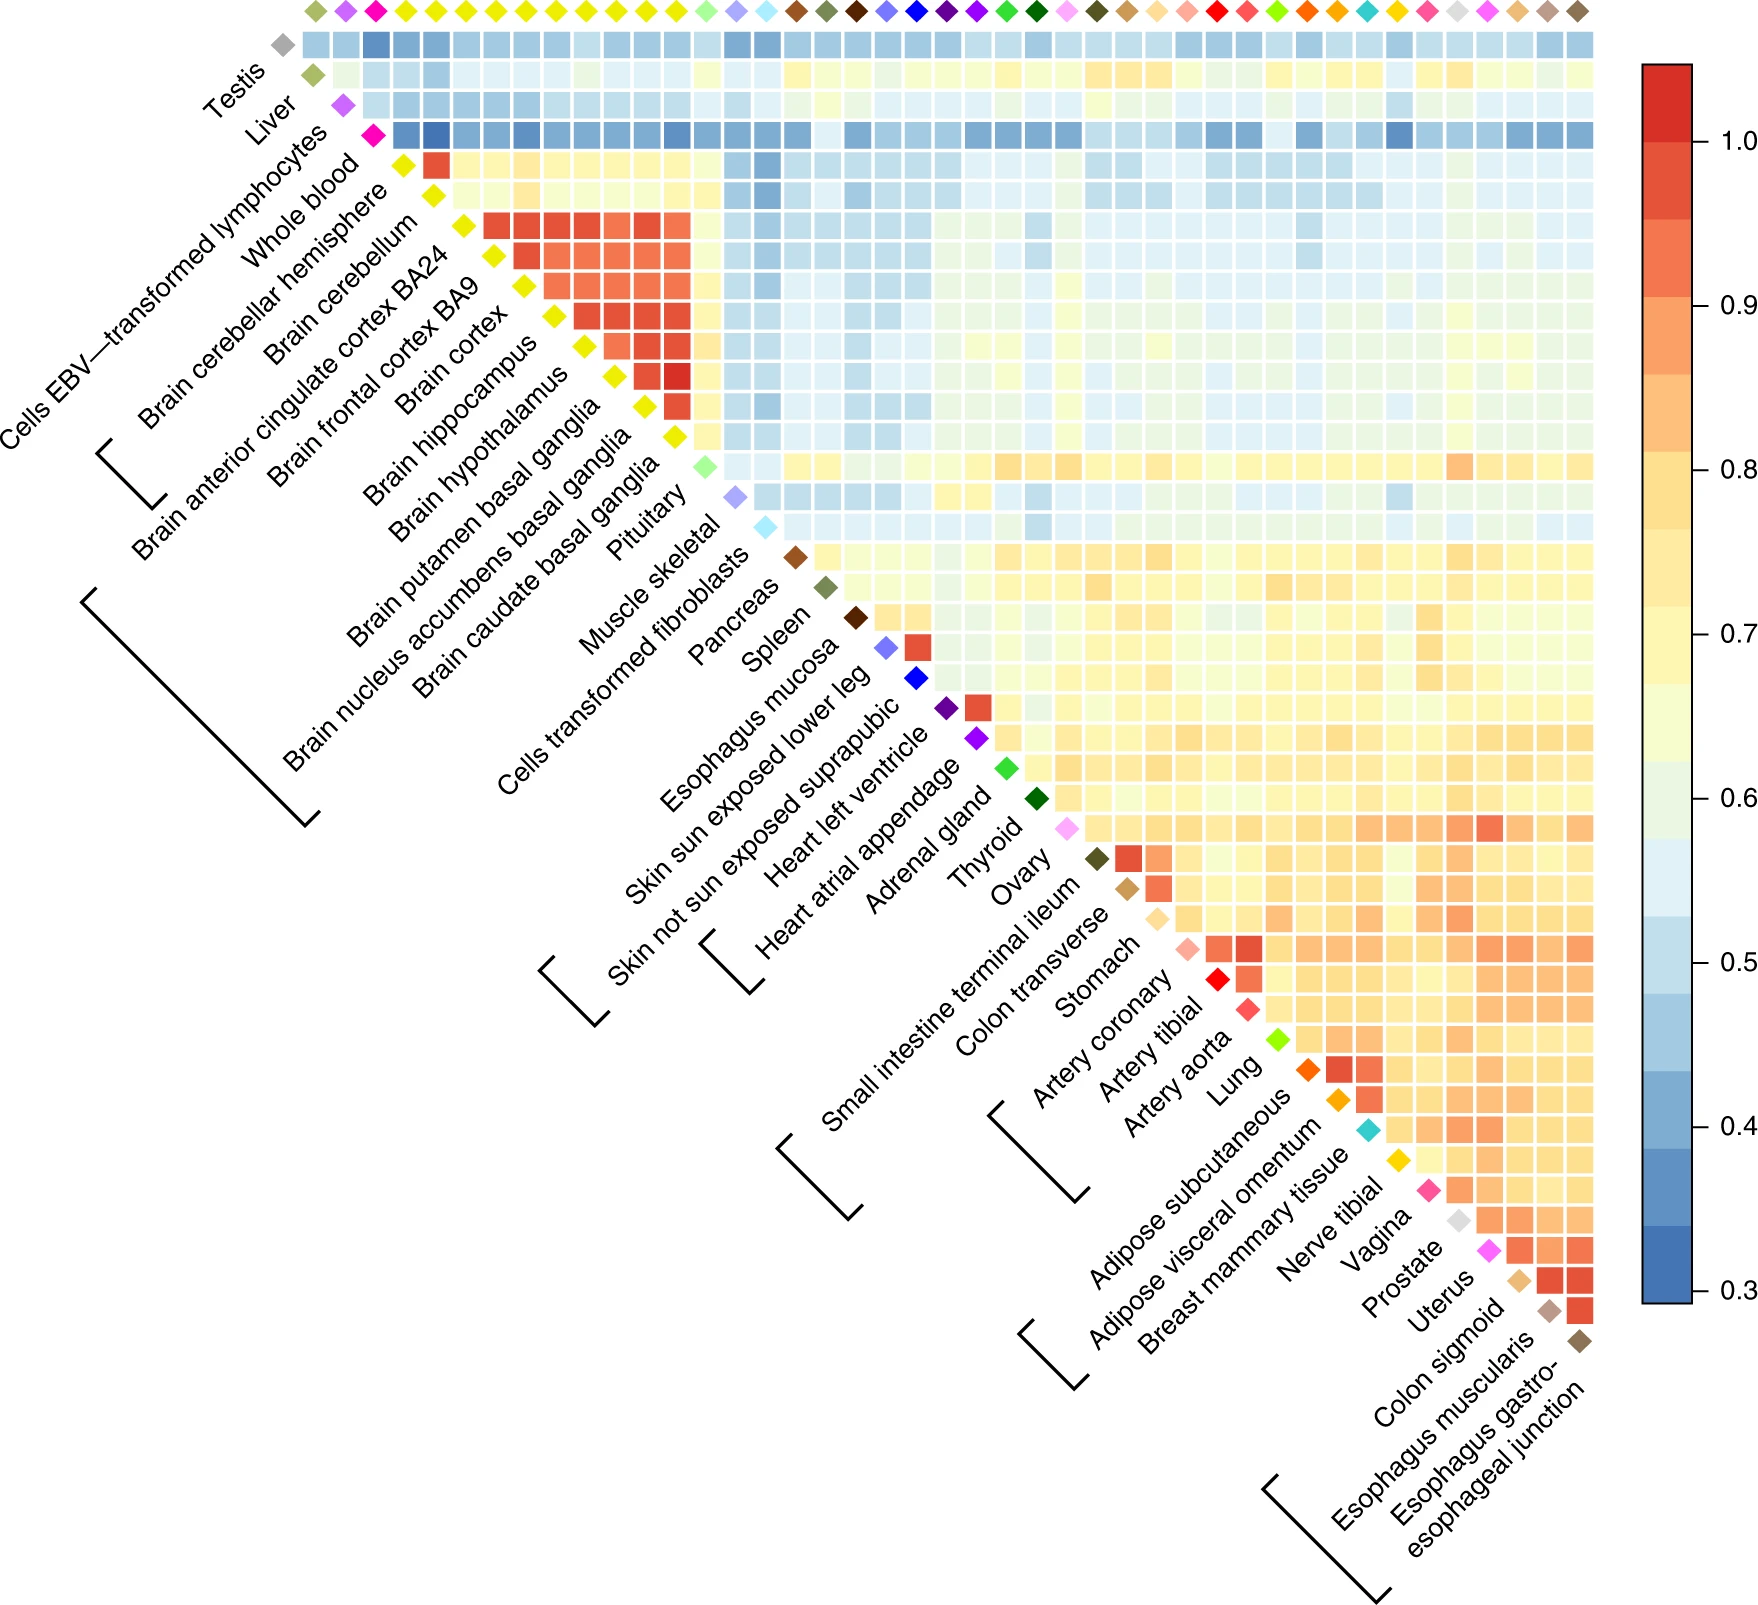
\includegraphics[width=0.62\linewidth]{slides/mash_tissue_correlation.png}
  \caption{Correlation between tissues of cis-eQTL effects in GTEx, estimated by mash. The colour scale starts at 0.3: all tissue pairs are positively correlated. Reproduced from \citet{urbut2019}.}
  \label{fig:mash_heatmap}
\end{figure}

Counting the number of tissues in which each eQTL is active gives a U-shaped distribution: most eQTLs are either specific to one or a few tissues or active in nearly all of them~\citep{gtex2017}. One explanation is the type of regulatory element. A promoter is used by its gene in every tissue in which the gene is expressed, so a promoter variant can act everywhere, while enhancers are often tissue-specific, so an enhancer variant acts only where its enhancer is active. Tissue-specific eQTLs are often shared between tissues with similar cell types. This suggests that the transcription factors that mediate eQTLs tend to be either constitutive or highly specific. Trans-eQTLs appear more tissue-specific than cis-eQTLs, although their lower power makes this hard to establish.

\subsection{Cell type composition and interaction QTLs}
\label{sec:interaction}

Most eQTL atlases are built from bulk tissue, which mixes many cell types, and the proportions vary between samples. Deconvolution methods, such as CIBERSORT (Chapter 8) or the enrichment scores of xCell~\citep{aran2017}, estimate the abundance of each cell type from expression. In GTEx they recover the expected patterns, such as hepatocytes in liver, keratinocytes in skin, myocytes in skeletal muscle, neurons in brain and neutrophils in blood, spleen and lung, and the similarity of tissues in cell type composition correlates with their similarity in eQTL and sQTL sharing~\citep{kimhellmuth2020}. Cell type composition is a major driver of variation in bulk expression between individuals.

If an eQTL acts in only one cell type, its effect in bulk tissue scales with that cell type's proportion. An \emph{interaction QTL} test looks for this,
\begin{equation}
  y_n = \mu + \beta_g g_n + \beta_c c_n + \beta_{gc}\,g_n c_n + \epsilon_n,
  \label{eq:ieqtl}
\end{equation}
where $c_n$ is the estimated proportion (or enrichment score) of the cell type in sample $n$, $\beta_c$ its effect on expression, and $\beta_{gc}$ the interaction: how much the genetic effect changes per unit change in cell type proportion. Testing $\beta_{gc}=0$ identifies cell type interacting eQTLs, many of which turn out to be cell type-specific eQTLs~\citep{kimhellmuth2020}. The test has limited power, because it depends on variation in proportions between samples and on noisy proportion estimates. Single-cell eQTL studies measure cell type-specific effects directly but are so far smaller and cover few tissues. The same interaction model applies to any measured context, such as age, sex, or a stimulus, which we meet again in Section~\ref{sec:coloc}.

%======================================================================
\section{Which variants are causal? Genomic annotations}
\label{sec:annotations}
%======================================================================

Fine-mapping one gene at a time is limited by LD. Pooling information across all genes can help, because the properties that make a variant more likely to be causal, such as lying in accessible chromatin or near the TSS, are shared. \citet{gaffney2012} built a hierarchical model that learns these properties from eQTL data and uses them as a prior for fine-mapping.

For gene $p$ with $M_p$ SNPs in its cis window, let $z_p\in\{0,1,\dots,M_p\}$ indicate the causal SNP, with $z_p=0$ if the gene has no eQTL; the model assumes at most one causal SNP per gene. Let $\va_{pm}\in\R^A$ be a vector of $A$ annotations of SNP $m$, such as indicators for overlapping a DNase I hypersensitive site, a histone mark peak or a predicted transcription factor binding site, and bins of distance to the TSS. The prior is
\begin{equation}
  \Pr(z_p\neq0) = \Pi, \qquad \Pr(z_p=m\mid z_p\neq0) = q_{pm} = \frac{\exp(\vlambda^\top\va_{pm})}{\sum_{m'=1}^{M_p}\exp(\vlambda^\top\va_{pm'})},
\end{equation}
a softmax over the SNPs in the window with annotation weights $\vlambda\in\R^A$, as in the multiclass logistic regression of Chapter 1. Holding the other annotations fixed, a SNP with annotation $a$ is $e^{\lambda_a}$ times more likely to be causal than one without, so $e^{\lambda_a}$ is the enrichment of the annotation. The data enter through the Bayes factor $\text{BF}_{pm}=p(\vy_p\mid z_p=m)/p(\vy_p\mid z_p=0)$ comparing the model in which SNP $m$ affects the expression $\vy_p\in\R^N$ of gene $p$ with the null model, computed from a single-SNP Bayesian regression. The marginal likelihood of gene $p$, relative to the null, is
\begin{equation}
  \frac{p(\vy_p\mid\Pi,\vlambda)}{p(\vy_p\mid z_p=0)} = (1-\Pi) + \Pi\sum_{m=1}^{M_p}q_{pm}\text{BF}_{pm},
\end{equation}
and the posterior probability that SNP $m$ is causal is
\begin{equation}
  r_{pm} = \Pr(z_p=m\mid\vy_p) = \frac{\Pi\,q_{pm}\text{BF}_{pm}}{(1-\Pi)+\Pi\sum_{m'}q_{pm'}\text{BF}_{pm'}}.
\end{equation}
$\Pi$ and $\vlambda$ are estimated by maximizing the product of the marginal likelihoods over all genes with EM. The E-step computes $r_{pm}$. The M-step sets $\Pi$ to the average of $\sum_m r_{pm}$ over genes and fits $\vlambda$ by maximizing $\sum_p\sum_m r_{pm}\log q_{pm}(\vlambda)$, a multiclass logistic regression in which each gene is one example, the classes are its SNPs and the labels are the soft posteriors $r_{pm}$ rather than observed causal variants. We never observe which variant is causal; the model learns from the noisy evidence summarized by the Bayes factors. The same structure is used for GWAS fine-mapping with annotations in Chapter 11.

Figure~\ref{fig:gaffney} shows the results for lymphoblastoid cell lines. SNPs in DNase I hypersensitive sites, which mark accessible chromatin, are about four times as likely to be causal as other SNPs, SNPs in H3K27ac and other active histone mark peaks are also enriched, and SNPs in regions marked by the repressive H3K27me3 are depleted. The enrichments hold for SNPs more than 5\,kb upstream of the TSS, which excludes promoters. The prior probability that a SNP is causal is highest at the TSS and falls quickly with distance, by an order of magnitude within a few tens of kilobases, and at every distance it is higher inside DNase sites. This is why a 1\,Mb window is generous for most eQTLs. Among transcription factors, SNPs in ChIP-seq peaks of factors such as JunD and NF-$\kappa$B are strongly enriched.

\begin{figure}[!htbp]
  \centering
  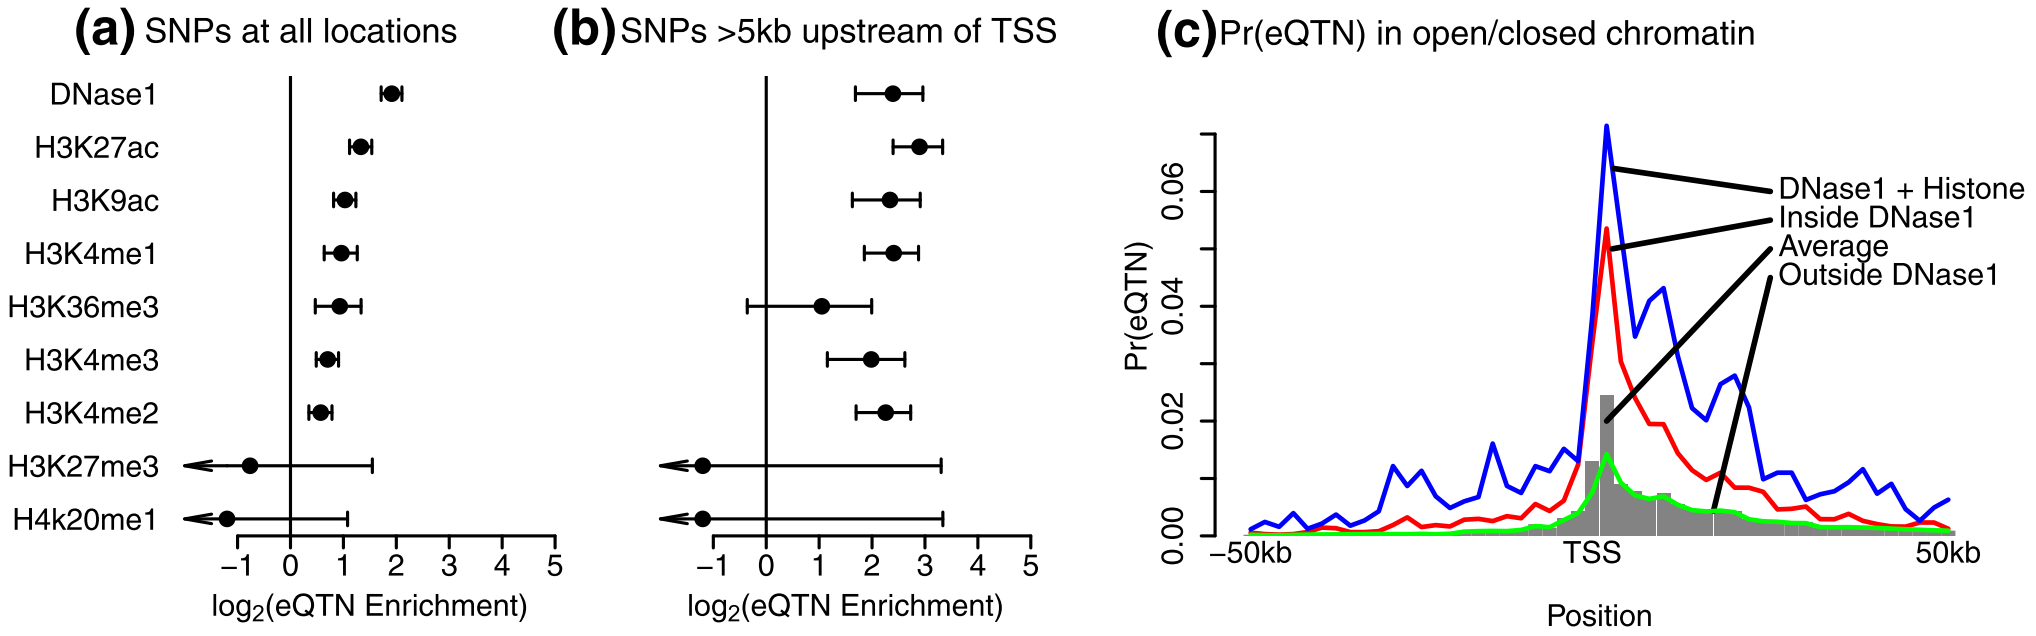
\includegraphics[width=\linewidth]{slides/gaffney_annotation_enrichment.png}
  \caption{Annotations of causal eQTL variants in lymphoblastoid cell lines. (a) Enrichment ($\log_2$, with 95\% intervals) of causal variants in DNase I hypersensitive sites and histone mark peaks, for all SNPs and (b) for SNPs more than 5\,kb upstream of the TSS. (c) Prior probability that a SNP is the causal variant as a function of position relative to the TSS, for SNPs in DNase sites and active histone marks (blue), in DNase sites (red), on average (grey) and outside DNase sites (green). Reproduced from \citet{gaffney2012}.}
  \label{fig:gaffney}
\end{figure}

Several related models exist. LirNet~\citep{lee2009lirnet} learns, across genes, how a SNP's regulatory features set the strength of its regularization in a sparse regression of expression on genotype. TORUS~\citep{wen2016} extends the hierarchical model to allow several causal SNPs per gene and controls a Bayesian FDR for eGene discovery. SuSiE~\citep{wang2020susie}, the sum of single effects model of Chapter 11, is now the most widely used fine-mapping method; it allows several causal variants, is fitted by coordinate ascent variational inference, and can take annotation-based priors such as those learned by TORUS.

Could sequence-based deep learning models (Chapters 2 and 3) replace this? Models such as Enformer predict the effects of a sequence on chromatin and expression, and so in principle predict the effect of every variant. They are good at predicting local features such as transcription factor binding and accessibility, and expression differences between genes, but not yet at predicting expression differences between individuals from their genotypes. \citet{sasse2023} compared predictions from personal genome sequences with measured brain expression: for most genes the correlation across individuals was near zero, and among genes with significant correlations, about a third had the wrong sign. The models often predict correctly that a variant matters but get the direction of its effect wrong.

%======================================================================
\section{Explaining GWAS associations with QTLs: colocalization}
\label{sec:coloc}
%======================================================================

A GWAS locus and an eQTL for a nearby gene overlap. Does that mean the gene mediates the disease association? Three questions need answers. Is there a significant eQTL in the locus at all? If so, are the GWAS and eQTL association patterns so similar that they probably share a causal variant, or could two different causal variants in LD produce overlapping signals by coincidence? And is the eQTL measured in the right tissue, cell type or cell state? \emph{Colocalization} analysis addresses the second question.

\subsection{The coloc model}

The coloc method~\citep{giambartolomei2014} considers a region of $M$ SNPs and two traits, say the expression of a gene (trait 1) and a disease (trait 2), measured in different samples. It assumes that each trait has at most one causal variant in the region, and compares five hypotheses (Figure~\ref{fig:coloc}):
\begin{itemize}
  \item $H_0$: no association with either trait;
  \item $H_1$: association with trait 1 only;
  \item $H_2$: association with trait 2 only;
  \item $H_3$: association with both traits, with two different causal variants;
  \item $H_4$: association with both traits, with one shared causal variant.
\end{itemize}
$H_4$ is what we hope to find. It does not prove that the gene causes the disease, since the shared variant could affect the disease through another gene, but it is a necessary condition. $H_3$ is the case a naive overlap analysis gets wrong.

Each hypothesis is a set of \emph{configurations}, which say which SNP, if any, is causal for each trait: one configuration for $H_0$, $M$ each for $H_1$, $H_2$ and $H_4$, and $M(M-1)$ for $H_3$. Each configuration gets a prior probability: $p_1$ for a configuration with a causal SNP for trait 1 only, $p_2$ for trait 2 only, $p_1p_2$ for two different causal SNPs, and $p_{12}$ for one shared SNP, with typical defaults $p_1=p_2=10^{-4}$ and $p_{12}=10^{-5}$. Because the two traits are measured in different samples, the likelihood factorizes over traits, and the Bayes factor of a configuration against $H_0$ is the product of a Bayes factor for each trait. Let $\text{BF}^{(1)}_m$ and $\text{BF}^{(2)}_m$ be the Bayes factors for SNP $m$ being the causal variant for traits 1 and 2. Summing over configurations, the posterior probabilities are proportional to
\begin{align}
  \Pr(H_0\mid D) &\propto 1, &
  \Pr(H_1\mid D) &\propto p_1\sum_m \text{BF}^{(1)}_m, \nonumber\\
  \Pr(H_2\mid D) &\propto p_2\sum_m \text{BF}^{(2)}_m, &
  \Pr(H_3\mid D) &\propto p_1p_2\sum_{m\neq m'}\text{BF}^{(1)}_m\text{BF}^{(2)}_{m'}, \nonumber\\
  \Pr(H_4\mid D) &\propto p_{12}\sum_m\text{BF}^{(1)}_m\text{BF}^{(2)}_m,
\end{align}
where $D$ denotes the data for both traits. The $H_3$ sum is computed as $\big(\sum_m\text{BF}^{(1)}_m\big)\big(\sum_{m'}\text{BF}^{(2)}_{m'}\big)-\sum_m\text{BF}^{(1)}_m\text{BF}^{(2)}_m$. $H_4$ wins when both traits put their Bayes factor mass on the same SNPs, and $H_3$ wins when they put it on different SNPs.

The Bayes factors need only summary statistics. Let $\hat\beta_m$ be the estimated effect of SNP $m$ on a trait, with sampling variance $V_m=\text{se}(\hat\beta_m)^2$, so $\hat\beta_m\mid\beta_m\sim\Normal(\beta_m,V_m)$. Under the null $\beta_m=0$, and under the alternative $\beta_m\sim\Normal(0,W)$ with prior variance $W$, so marginally $\hat\beta_m\sim\Normal(0,V_m+W)$. The ratio of the two densities is Wakefield's approximate Bayes factor~\citep{wakefield2009},
\begin{equation}
  \text{BF}_m = \frac{\Normal(\hat\beta_m;0,V_m+W)}{\Normal(\hat\beta_m;0,V_m)} = \sqrt{\frac{V_m}{V_m+W}}\exp\left(\frac{z_m^2}{2}\,\frac{W}{V_m+W}\right),
  \label{eq:abf-12}
\end{equation}
where $z_m=\hat\beta_m/\sqrt{V_m}$. It increases with $z_m^2$, and the prefactor penalizes the alternative for spreading its prior over effects that the data could have shown but did not. Under the single-causal-variant assumption, the Bayes factor of the configuration ``SNP $m$ is causal'' is $\text{BF}_m$ computed from the marginal statistics of SNP $m$ alone, so no LD matrix is needed. The assumption is restrictive when a locus has several causal variants; extensions combine coloc with SuSiE fine-mapping to test each pair of credible sets.

Figure~\ref{fig:coloc} shows coloc on simulated data, with an eQTL study of 500 individuals and a GWAS of 5000. When the same SNP is causal for both traits, the association patterns match and the posterior probability of $H_4$ is 0.99. When the GWAS causal variant is a different SNP in weak LD ($r^2=0.31$) with the eQTL causal variant, both traits show associations across the same region, but their peaks are at different SNPs, and the posterior probability of $H_3$ is 0.94.

\begin{figure}[!htbp]
  \centering
  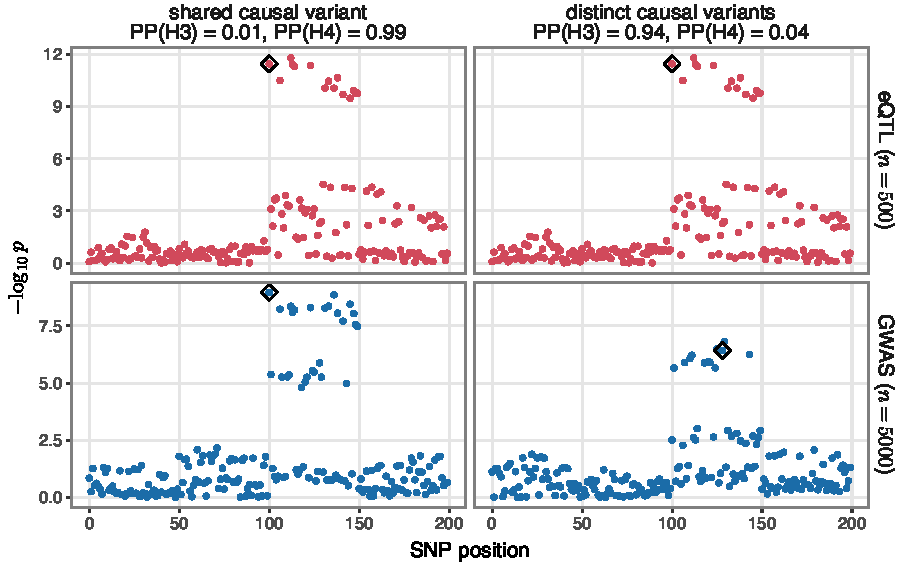
\includegraphics[width=0.9\linewidth]{coloc_example.pdf}
  \caption{Colocalization on simulated data. Association $-\log_{10}p$ along a region of 200 SNPs for an eQTL ($N=500$, red) and a GWAS ($N=5000$, blue); diamonds mark the causal variants. Left, one shared causal variant; right, distinct causal variants in weak LD. Panel titles give the coloc posterior probabilities of $H_3$ and $H_4$ with default priors and $W=0.15^2$.}
  \label{fig:coloc}
\end{figure}

\subsection{What colocalization has found}

The GTEx consortium ran colocalization for GWAS of many traits, including lipid levels, BMI and autoimmune diseases~\citep{gtex2017}. A substantial fraction of GWAS loci colocalize with an eQTL in at least one tissue, and the colocalizing gene is often not the gene nearest to the lead GWAS variant, as for \textit{FTO}, \textit{IRX3} and \textit{IRX5}. Many loci, however, do not colocalize with any eQTL. Some of this gap is power, but some is because eQTL studies measure the wrong context. Expression effects relevant to an immune disease may only appear when immune cells respond to a challenge, while blood samples contain mostly resting cells. \citet{kimhellmuth2017} stimulated monocytes from 134 donors with bacterial and viral ligands and found eQTLs that appeared only after stimulation, some of which colocalized with autoimmune disease associations that resting-cell eQTLs did not explain. The cell state can matter, not just the cell type.

Why does this matter? Drug targets with human genetic support are more likely to succeed in clinical trials (Chapter 1). The effects involved are small: a typical eQTL changes expression by perhaps 5--10\%, and each GWAS variant changes disease risk slightly, so these results are of little use for predicting who will get a disease. They do give a view of the causal biology of disease in humans, without the limitations of animal models and without a clinical trial.

%======================================================================
\section{Transcriptome-wide association studies}
%======================================================================

A transcriptome-wide association study (TWAS)~\citep{gamazon2015,gusev2016} links expression to a trait through genetically predicted expression (Figure~\ref{fig:twas}). In a \emph{reference panel} with genotypes and expression, we train a model to predict each gene's expression from the genotypes of its cis SNPs,
\begin{equation}
  e_n = \vx_n^\top\vw + \epsilon_n,
\end{equation}
where $e_n$ is the expression of the gene in individual $n$ of the panel, $\vx_n\in\R^M$ holds the standardized genotypes of the $M$ cis SNPs and $\vw\in\R^M$ the weights, usually fitted with the elastic net or lasso of Chapter 1, or with a Bayesian sparse regression. In a GWAS cohort, which has genotypes and the trait but no expression, we then impute expression, $\hat e_n=\vx_n^\top\hat\vw$, and test the association between $\hat e_n$ and the trait.

\begin{figure}[!htbp]
  \centering
  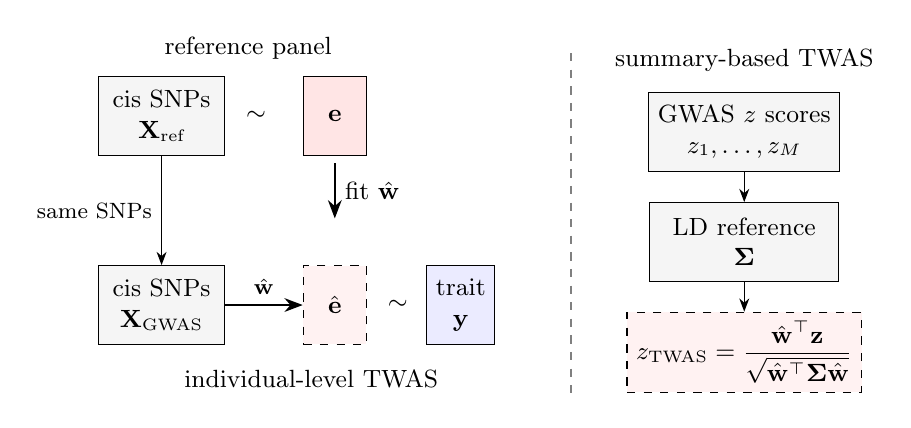
\begin{tikzpicture}[>=Stealth, every node/.style={font=\small},
      mat/.style={draw, minimum width=1.6cm, minimum height=1.0cm, align=center, fill=gray!8}]
    \node[mat] (gref) at (0,0) {cis SNPs\\$\mX_{\text{ref}}$};
    \node[mat, fill=red!10, minimum width=0.8cm] (eref) at (2.2,0) {$\ve$};
    \node at (1.2,0) {$\sim$};
    \node[above] at (1.1,0.6) {reference panel};
    \draw[->, thick] (2.2,-0.6) -- (2.2,-1.3) node[midway, right] {fit $\hat\vw$};
    \node[mat] (ggw) at (0,-2.4) {cis SNPs\\$\mX_{\text{GWAS}}$};
    \node[mat, fill=red!5, minimum width=0.8cm, dashed] (ehat) at (2.2,-2.4) {$\hat\ve$};
    \node[mat, fill=blue!8, minimum width=0.8cm] (trait) at (3.8,-2.4) {trait\\$\vy$};
    \draw[->] (gref.south) -- (ggw.north) node[midway, left] {\footnotesize same SNPs};
    \draw[->, thick] (ggw) -- (ehat) node[midway, above] {\footnotesize$\hat\vw$};
    \node at (3.0,-2.4) {$\sim$};
    \node[below, align=center] at (1.9,-3.1) {individual-level TWAS};
    % summary based
    \node[mat, minimum width=2.4cm] (z) at (7.4,-0.2) {GWAS $z$ scores\\$z_1,\dots,z_M$};
    \node[mat, minimum width=2.4cm] (ld) at (7.4,-1.6) {LD reference\\$\mSigma$};
    \node[mat, fill=red!5, dashed, minimum width=2.6cm] (zt) at (7.4,-3.0) {$z_{\text{TWAS}}=\dfrac{\hat\vw^\top\vz}{\sqrt{\hat\vw^\top\mSigma\hat\vw}}$};
    \draw[->] (z) -- (ld); \draw[->] (ld) -- (zt);
    \node[above] at (7.4,0.45) {summary-based TWAS};
    \draw[dashed, gray] (5.2,0.8) -- (5.2,-3.6);
  \end{tikzpicture}
  \caption{Transcriptome-wide association study. Left: weights $\hat\vw$ predicting a gene's expression from cis SNPs are learned in a reference panel, used to impute expression in a GWAS cohort, and imputed expression is tested for association with the trait. Right: the same test computed from GWAS summary statistics and an LD reference. After \citet{gusev2016}.}
  \label{fig:twas}
\end{figure}

Individual-level GWAS data are often unavailable, but the test can be computed from GWAS summary statistics~\citep{gusev2016}. Let $\mX\in\R^{N\times M}$ be the standardized cis genotypes of the $N$ GWAS individuals and $\vy\in\R^N$ the standardized trait. The marginal $z$ score of SNP $m$ is approximately $z_m=\vx_m^\top\vy/\sqrt N$, where $\vx_m$ is column $m$ of $\mX$, so $\vz=\mX^\top\vy/\sqrt N$. The imputed expression is $\hat\ve=\mX\hat\vw$, with sample variance $\hat\vw^\top\mSigma\hat\vw$, where $\mSigma=\mX^\top\mX/N$ is the LD (correlation) matrix of the SNPs. The $z$ score for the association of $\hat\ve$ with $\vy$ is
\begin{equation}
  z_{\text{TWAS}} = \frac{\hat\ve^\top\vy}{\sqrt N\sqrt{\hat\vw^\top\mSigma\hat\vw}} = \frac{\hat\vw^\top\mX^\top\vy/\sqrt N}{\sqrt{\hat\vw^\top\mSigma\hat\vw}} = \frac{\hat\vw^\top\vz}{\sqrt{\hat\vw^\top\mSigma\hat\vw}},
  \label{eq:twas}
\end{equation}
a weighted sum of the GWAS $z$ scores, normalized by its null standard deviation: under the null $\vz\sim\Normal(\vzero,\mSigma)$, so $\Var(\hat\vw^\top\vz)=\hat\vw^\top\mSigma\hat\vw$. The LD matrix comes from a reference sample of the same ancestry.

TWAS has two attractions. It is signed: the sign of $z_{\text{TWAS}}$ says whether higher genetically predicted expression increases or decreases risk, which is what we need to know to design a drug that inhibits or activates a target. And it is protected against reverse causation. Expression measured in patients reflects the disease as well as causing it; in Alzheimer's disease, for example, microglia in the brain respond to the damage, so much of the expression difference between cases and controls is a consequence of the disease. Genetically predicted expression is fixed at conception and cannot be changed by the disease.

Figure~\ref{fig:twas_pd} shows a TWAS of Parkinson's disease~\citep{li2018leafcutter}, using 537 dorsolateral prefrontal cortex RNA-seq samples from the CommonMind consortium~\citep{fromer2016} as the reference panel and a GWAS of about 14{,}000 cases and 95{,}000 controls~\citep{nalls2014}. With predicted splicing (intron usage quantified by LeafCutter, Chapter 10) as well as predicted expression, 26 genes were associated through splicing and 18 through expression at 5\% FDR. The strongest signal was splicing of \textit{MAPT}, which encodes tau.

\begin{figure}[!htbp]
  \centering
  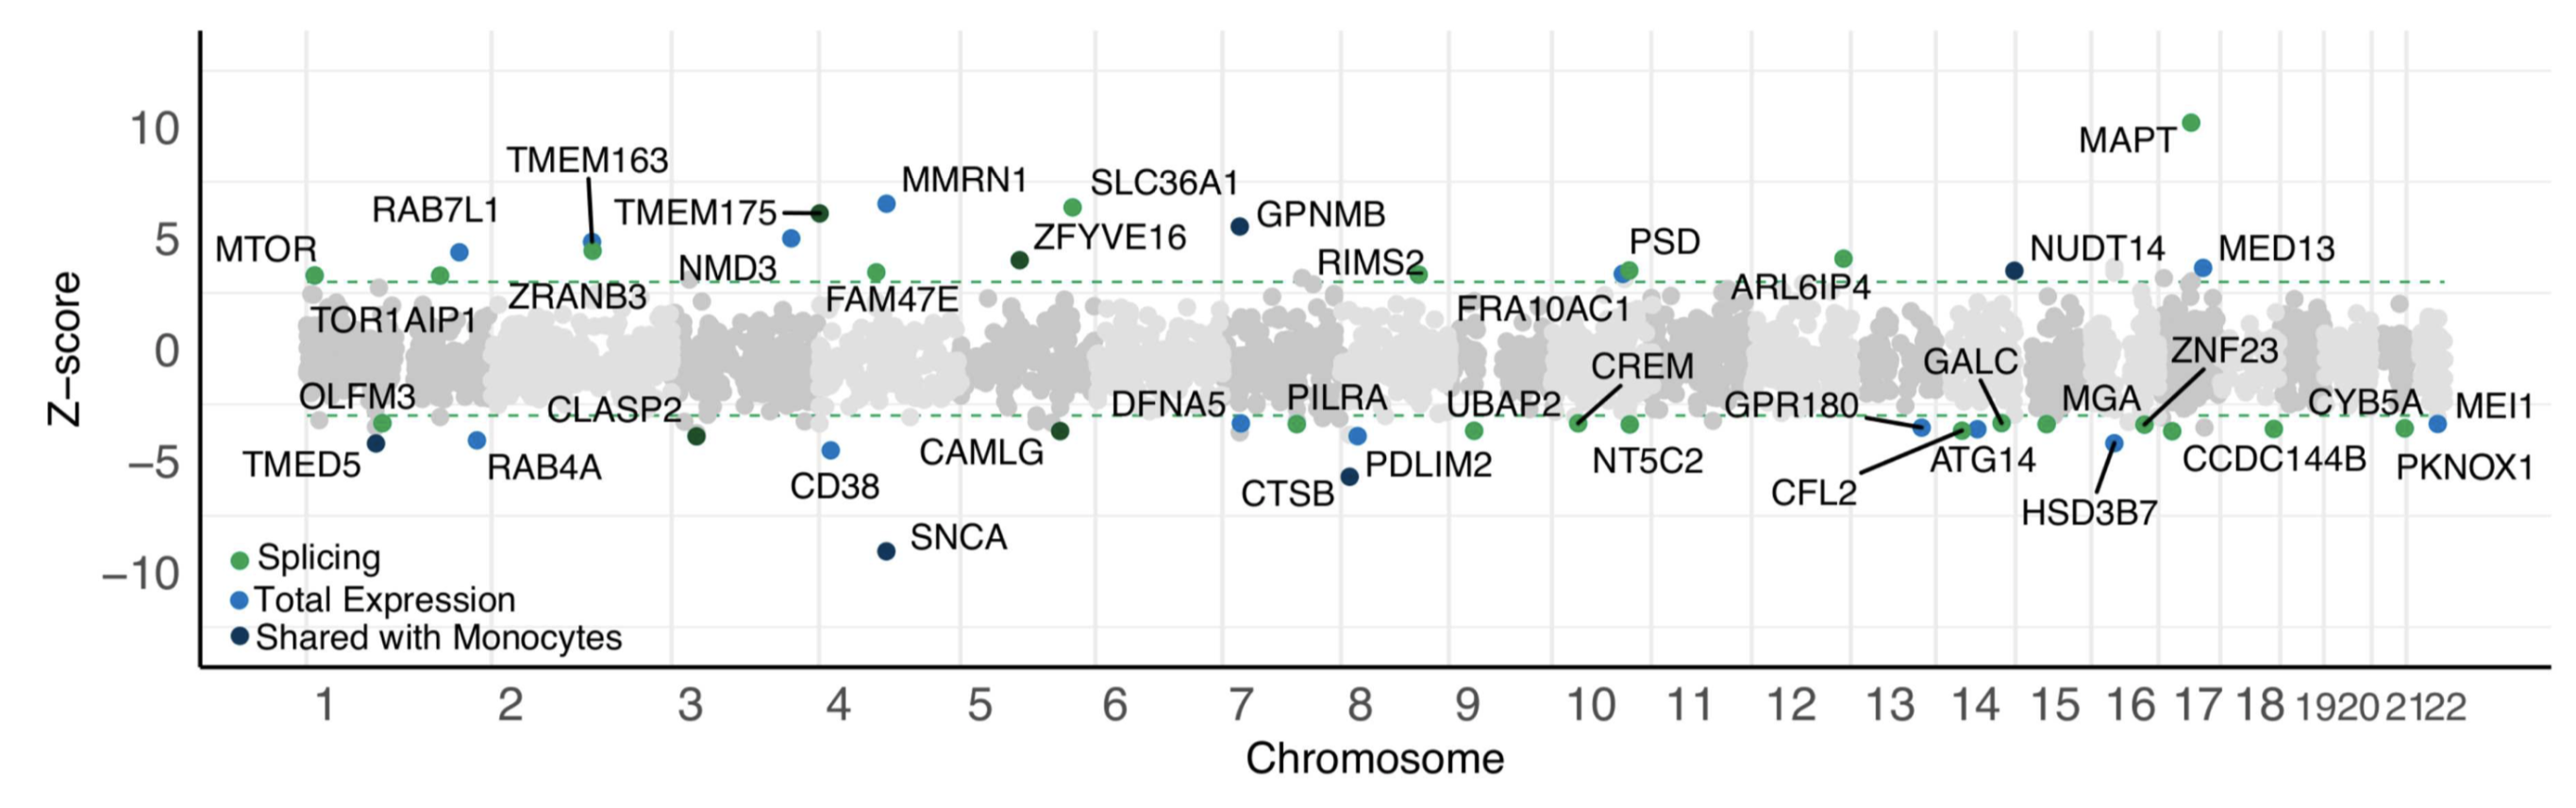
\includegraphics[width=0.85\linewidth]{slides/twas_parkinsons.png}
  \caption{TWAS of Parkinson's disease using brain expression (blue) and splicing (green) reference panels; dark points are associations shared with monocytes. Each point is a gene's TWAS $z$ score along the genome; dashed lines mark significance at 5\% FDR. Reproduced from \citet{li2018leafcutter}.}
  \label{fig:twas_pd}
\end{figure}

TWAS inherits the limitations of its components. Genes in the same locus have correlated predicted expression, because they share cis SNPs and LD, so a TWAS association, like an overlapping eQTL, can be driven by a neighbouring gene or by a variant acting through another mechanism. TWAS assumes the variants in the predictor affect the trait only through the gene's expression. This is the central assumption of Mendelian randomization, to which TWAS is closely related.

%======================================================================
\section{Mendelian randomization}
%======================================================================

\subsection{Instrumental variables}

Mendelian randomization (MR)~\citep{daveysmith2003} estimates the causal effect of an \emph{exposure} $X$, such as the expression of a gene or a biomarker like LDL cholesterol, on an \emph{outcome} $Y$, such as disease risk. The problem is the usual one of observational data: an association between $X$ and $Y$ can be due to a confounder $U$ that affects both, or to reverse causation. MR uses a genetic variant $G_j$ associated with the exposure as an \emph{instrumental variable} (Figure~\ref{fig:mr_dag}). Alleles are assigned at random at conception, given the parents' genotypes, much as treatments are in a randomized trial, hence the name. The instrument is valid under three assumptions:
\begin{enumerate}
  \item \emph{relevance}: $G_j$ is associated with $X$;
  \item \emph{independence}: $G_j$ is not associated with any confounder $U$ of $X$ and $Y$;
  \item \emph{exclusion restriction}: $G_j$ affects $Y$ only through $X$, with no direct (pleiotropic) path.
\end{enumerate}
In an eQTL setting, the exposure is the expression of a gene and the instrument is a cis-eQTL, which makes the first assumption easy to check and the third plausible but not guaranteed.

\begin{figure}[!htbp]
  \centering
  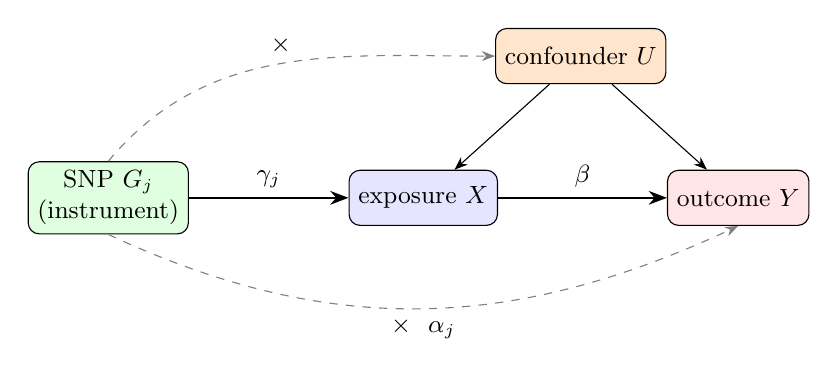
\begin{tikzpicture}[>=Stealth, every node/.style={font=\small}, var/.style={draw, rounded corners, minimum width=1.5cm, minimum height=0.7cm, align=center}]
    \node[var, fill=green!12] (g) at (0,0) {SNP $G_j$\\(instrument)};
    \node[var, fill=blue!10] (x) at (4,0) {exposure $X$};
    \node[var, fill=red!10] (y) at (8,0) {outcome $Y$};
    \node[var, fill=orange!20] (u) at (6,1.8) {confounder $U$};
    \draw[->, thick] (g) -- node[above] {$\gamma_j$} (x);
    \draw[->, thick] (x) -- node[above] {$\beta$} (y);
    \draw[->] (u) -- (x); \draw[->] (u) -- (y);
    \draw[->, dashed, gray] (g.north) to[out=50, in=180] node[midway, above, black] {$\times$} (u.west);
    \draw[->, dashed, gray] (g.south) to[out=-25, in=-155] node[midway, below, black] {$\times$ \ $\alpha_j$} (y.south);
  \end{tikzpicture}
  \caption{Mendelian randomization. A SNP $G_j$ affects the exposure $X$ with effect $\gamma_j$, and $X$ affects the outcome $Y$ with causal effect $\beta$. The SNP must not be associated with the confounder $U$, and must have no direct effect $\alpha_j$ on the outcome (crossed dashed paths).}
  \label{fig:mr_dag}
\end{figure}

\subsection{The ratio estimate}

Write a linear model for the exposure and the outcome,
\begin{equation}
  X = \gamma_jG_j + U + \epsilon_X, \qquad Y = \beta X + \alpha_jG_j + \kappa U + \epsilon_Y,
\end{equation}
where $\gamma_j$ is the effect of SNP $j$ on the exposure, $\beta$ the causal effect of the exposure on the outcome, $\alpha_j$ a direct (pleiotropic) effect of the SNP on the outcome, $\kappa$ the effect of the confounder, and $\epsilon_X,\epsilon_Y$ independent noise. Under the independence assumption $\Cov(G_j,U)=0$, so
\begin{align}
  \Cov(G_j,X) &= \gamma_j\Var(G_j), \\
  \Cov(G_j,Y) &= \beta\Cov(G_j,X) + \alpha_j\Var(G_j) = (\beta\gamma_j+\alpha_j)\Var(G_j).
\end{align}
The regression coefficients of the exposure and the outcome on the SNP are therefore $\gamma_j$ and $\Gamma_j=\beta\gamma_j+\alpha_j$, and these are exactly what GWAS of the exposure and of the outcome estimate. The confounder has dropped out. If the exclusion restriction holds, $\alpha_j=0$ and the \emph{ratio} (Wald) estimate
\begin{equation}
  \hat\beta_j = \frac{\hat\Gamma_j}{\hat\gamma_j} = \frac{\hat\beta_{\text{SNP}\to\text{outcome}}}{\hat\beta_{\text{SNP}\to\text{exposure}}}
\end{equation}
is a consistent estimate of $\beta$. With pleiotropy it estimates $\beta+\alpha_j/\gamma_j$, biased by an amount that is larger for weaker instruments.

\subsection{Multiple instruments}

With $J$ independent instruments (SNPs not in LD with each other), the inverse-variance weighted (IVW) estimate~\citep{burgess2013} combines the ratio estimates. Treating $\hat\gamma_j$ as known and $\text{se}(\hat\beta_j)\approx\text{se}(\hat\Gamma_j)/|\hat\gamma_j|$, weighting each ratio by its inverse variance gives
\begin{equation}
  \hat\beta_{\text{IVW}} = \frac{\sum_j \hat\beta_j\,\hat\gamma_j^2\sigma_j^{-2}}{\sum_j\hat\gamma_j^2\sigma_j^{-2}} = \frac{\sum_j\hat\gamma_j\hat\Gamma_j\sigma_j^{-2}}{\sum_j\hat\gamma_j^2\sigma_j^{-2}},
\end{equation}
where $\sigma_j=\text{se}(\hat\Gamma_j)$. This is the weighted least-squares slope of a regression of $\hat\Gamma_j$ on $\hat\gamma_j$ through the origin. If the pleiotropic effects $\alpha_j$ average to zero (balanced pleiotropy), IVW is still consistent. If they do not (directional pleiotropy, mean $\mu_\alpha\neq0$), IVW is biased.

MR-Egger regression~\citep{bowden2015} relaxes the assumption. Writing $\alpha_j=\mu_\alpha+(\alpha_j-\mu_\alpha)$,
\begin{equation}
  \Gamma_j = \mu_\alpha + \beta\gamma_j + (\alpha_j-\mu_\alpha).
\end{equation}
If the pleiotropic effects are independent of the instrument strengths $\gamma_j$ across SNPs (the InSIDE assumption, instrument strength independent of direct effect), the last term is uncorrelated with $\gamma_j$, and a weighted regression of $\hat\Gamma_j$ on $\hat\gamma_j$ \emph{with an intercept} estimates the causal effect $\beta$ as its slope and the average pleiotropy $\mu_\alpha$ as its intercept. Before fitting, each SNP is oriented so that $\hat\gamma_j>0$; otherwise the intercept would depend on the arbitrary choice of reference allele. A non-zero intercept is evidence of directional pleiotropy. Figure~\ref{fig:mr_egger} shows simulated data in which all SNPs have a small positive direct effect on the outcome: IVW overestimates the causal effect (0.30 against a true 0.2), while the Egger slope is closer (0.24) and its intercept (0.012) estimates the mean direct effect (0.018 in this sample).

\begin{figure}[!htbp]
  \centering
  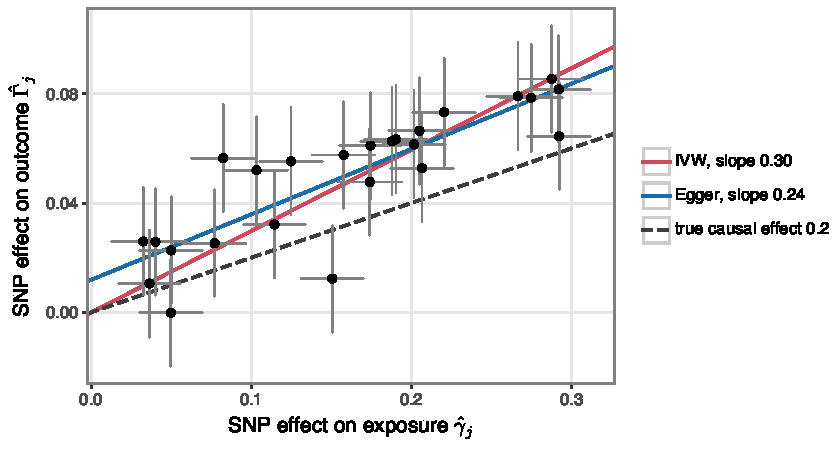
\includegraphics[width=0.8\linewidth]{mr_egger.pdf}
  \caption{IVW and Egger regression on 25 simulated instruments with directional pleiotropy. Each point is a SNP's estimated effects on the exposure and the outcome, with 95\% intervals. IVW (red) is a regression through the origin and is biased by the positive direct effects; Egger regression (blue) has an intercept and its slope is closer to the true causal effect (dashed).}
  \label{fig:mr_egger}
\end{figure}

The InSIDE assumption fails when pleiotropy is \emph{correlated}: if some SNPs affect both exposure and outcome through a shared heritable factor, their direct effects are correlated with their effects on the exposure, and the Egger slope is biased too. CAUSE~\citep{morrison2020} models a mixture of SNPs with and without such shared effects, and Welch-weighted Egger regression~\citep{brown2021welch} reduces the resulting false positives. All these methods need several valid or nearly valid instruments, and molecular exposures often have only one or two strong cis instruments.

TWAS and MR are closely related. The TWAS statistic~\eqref{eq:twas} is a weighted combination of SNP-outcome associations with weights from the SNP-exposure model, and with a single SNP it is the GWAS $z$ score of that SNP, whose ratio to the eQTL effect is the MR estimate. TWAS tests $\beta=0$ while MR estimates $\beta$, and both rely on the exclusion restriction.

\subsection{Causal networks}

Molecular phenotypes come in large numbers: thousands of genes, splicing events, proteins and metabolites, as well as complex traits. MR between every pair gives a matrix of pairwise causal effect estimates, but these are \emph{total} effects, which include all paths through other phenotypes. We would often rather know the \emph{direct} effects, the edges of a causal network (Figure~\ref{fig:networks}).

\begin{figure}[!htbp]
  \centering
  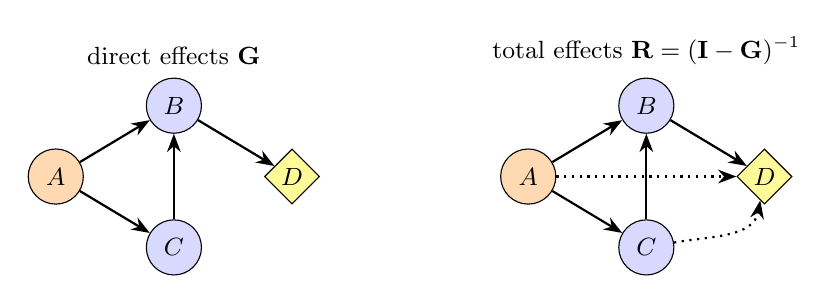
\begin{tikzpicture}[>=Stealth, every node/.style={font=\small}, nd/.style={circle, draw, fill=blue!15, minimum size=0.7cm}]
    \begin{scope}
      \node[above] at (1.5,1.3) {direct effects $\mG$};
      \node[nd, fill=orange!30] (a) at (0,0) {$A$};
      \node[nd] (b) at (1.5,0.9) {$B$};
      \node[nd] (c) at (1.5,-0.9) {$C$};
      \node[nd, fill=yellow!40, diamond, inner sep=1pt] (d) at (3.0,0) {$D$};
      \draw[->, thick] (a) -- (b); \draw[->, thick] (a) -- (c);
      \draw[->, thick] (c) -- (b); \draw[->, thick] (b) -- (d);
    \end{scope}
    \begin{scope}[xshift=6cm]
      \node[above] at (1.5,1.3) {total effects $\mR=(\mI-\mG)^{-1}$};
      \node[nd, fill=orange!30] (a) at (0,0) {$A$};
      \node[nd] (b) at (1.5,0.9) {$B$};
      \node[nd] (c) at (1.5,-0.9) {$C$};
      \node[nd, fill=yellow!40, diamond, inner sep=1pt] (d) at (3.0,0) {$D$};
      \draw[->, thick] (a) -- (b); \draw[->, thick] (a) -- (c);
      \draw[->, thick] (c) -- (b); \draw[->, thick] (b) -- (d);
      \draw[->, dotted, thick] (a) -- (d);
      \draw[->, dotted, thick] (c) to[out=10, in=-100] (d);
    \end{scope}
  \end{tikzpicture}
  \caption{Direct and total effects. Left, a network of direct causal effects in which a transcription factor $A$ regulates genes $B$ and $C$, $C$ regulates $B$, and $B$ affects a trait $D$. Right, the total effects estimated by pairwise MR include indirect effects (dotted), such as $A$ on $D$ through $B$, and $A$ on $B$ both directly and through $C$.}
  \label{fig:networks}
\end{figure}

A linear structural model relates the two. Let $\mY\in\R^{N\times D}$ hold $D$ phenotypes for $N$ individuals and $\mG\in\R^{D\times D}$ the direct effects, with $G_{ij}$ the effect of phenotype $i$ on phenotype $j$ and $G_{ii}=0$. Each phenotype is a linear function of the others plus external perturbations $\mE\in\R^{N\times D}$, which include the effects of genetic instruments and environment,
\begin{equation}
  \mY = \mY\mG + \mE \quad\Rightarrow\quad \mY(\mI-\mG) = \mE \quad\Rightarrow\quad \mY = \mE(\mI-\mG)^{-1}.
\end{equation}
A unit perturbation of phenotype $i$ (row vector $\mE$ with a one in position $i$) therefore changes phenotype $j$ by $[(\mI-\mG)^{-1}]_{ij}$, the total effect. When the network has no feedback loops strong enough to make the series diverge,
\begin{equation}
  (\mI-\mG)^{-1} = \mI + \mG + \mG^2 + \mG^3 + \cdots,
\end{equation}
and $[\mG^2]_{ij}=\sum_kG_{ik}G_{kj}$ sums the paths of length two from $i$ to $j$. In the network of Figure~\ref{fig:networks}, the total effect of $A$ on $B$ is $G_{AB}+G_{AC}G_{CB}$, the direct edge plus the path through $C$, and the total effect of $A$ on $D$ is $(G_{AB}+G_{AC}G_{CB})G_{BD}$.

MR estimates the total effect of a perturbation that changes $i$ by one unit, so the matrix of MR estimates is $\mR=\mD^{-1}(\mI-\mG)^{-1}$ with $\mD$ the diagonal of $(\mI-\mG)^{-1}$, normalizing each row so that $R_{ii}=1$. Then $\mR^{-1}=(\mI-\mG)\mD$, whose off-diagonal entries are $-G_{ij}D_{jj}$ and diagonal entries $D_{ii}$. A sparse network $\mG$ therefore means a sparse inverse of $\mR$, and the direct effects are recovered as $G_{ij}=-[\mR^{-1}]_{ij}/[\mR^{-1}]_{jj}$. Inverting a noisy estimate $\hat\mR$ directly amplifies the noise, so bimmer~\citep{brown2020bimmer} and its successor inspre~\citep{brown2023inspre} solve a regularized problem,
\begin{equation}
  \min_{\mU,\mV}\ \sum_{i,j}w_{ij}\big(\hat R_{ij}-U_{ij}\big)^2 + \lambda\|\mV\|_1 \quad\text{subject to}\quad \mU\mV=\mI,
\end{equation}
where $\mU\in\R^{D\times D}$ is a denoised version of $\hat\mR$, $\mV=\mU^{-1}$ is its sparse inverse, $w_{ij}\geq0$ are weights reflecting the precision of each MR estimate (zero for missing entries), and $\|\mV\|_1=\sum_{ij}|V_{ij}|$. The problem is biconvex (convex in $\mU$ for fixed $\mV$ and vice versa) and is solved with the alternating direction method of multipliers (ADMM)~\citep{boyd2011admm}. It is the directed analogue of the graphical lasso of Chapter 9~\citep{friedman2008}, which finds a sparse inverse of a covariance matrix, and $\lambda$ is chosen by a stability criterion adapted from StARS~\citep{liu2010stars}. In simulations of random, hub-like and scale-free directed networks, this approach recovers the network much more accurately than estimating each node's parents by sparse regression on pairwise MR estimates. Applied with CRISPR knockdowns as the perturbations instead of genetic instruments, the same method estimates gene regulatory networks from Perturb-seq data~\citep{brown2023inspre}.

%======================================================================
\section{Summary}
%======================================================================

\begin{itemize}
  \item Molecular QTLs are associations between genotype and molecular phenotypes such as expression (eQTLs), splicing (sQTLs) and chromatin accessibility (caQTLs). They help interpret GWAS loci, most of which are non-coding, by suggesting causal genes, tissues and cell types, as in the \textit{FTO} locus, where the obesity variants regulate \textit{IRX3} and \textit{IRX5} in adipocyte progenitors.
  \item eQTLs are mapped by linear regression of normalized expression on genotype, usually for SNPs within 1\,Mb of each gene. Multiple testing is handled at two levels: within a gene by Bonferroni or permutation, which accounts for LD, and across genes by FDR control.
  \item Technical and biological confounders affect many genes at once and can be estimated as hidden factors with a factor model with an ARD prior (PEER) or by PCA. Regressing them out greatly increases power for cis-eQTLs but can remove trans signals and context-specific biology.
  \item Cis-eQTLs are common, large and easy to find with tens to hundreds of individuals; trans-eQTLs are small and need thousands. LD makes the causal variant hard to identify; fine-mapping and genome-wide annotation enrichment, which shows causal variants concentrated in accessible chromatin near the TSS, help.
  \item Allele-specific expression compares the two haplotypes within an individual, a built-in control for environmental and technical variation that isolates cis effects. Overdispersed counts are modelled with the beta-binomial (allelic counts) and negative binomial (total counts), and combining the two signals gains power, especially in small samples. QQ plots check calibration.
  \item Tissue atlases show that most genes have cis-eQTLs, often several, that eQTLs are mostly either shared across tissues or specific to a few, and that comparing significance between tissues is misleading; mash models effects jointly. Cell type composition shapes bulk eQTLs, and interaction models can recover cell type-specific effects.
  \item Colocalization tests whether a GWAS and an eQTL signal share a causal variant; TWAS associates genetically predicted expression with a trait; Mendelian randomization estimates causal effects using SNPs as instrumental variables, with Egger and related methods relaxing the no-pleiotropy assumption. Extending MR to many phenotypes leads to sparse causal network inference.
\end{itemize}

%======================================================================
\section*{Exercises}
%======================================================================

\begin{enumerate}
  \item Show that under the null, with $M$ independent SNPs, $\Pr(p_{\min}\leq t)=1-(1-t)^M$, and that the Bonferroni threshold $t=0.05/M$ gives a family-wise error rate between 0.0488 and 0.05 for all $M\geq1$.
  \item Starting from~\eqref{eq:betabinom}, show that $\Pr(y\mid d,\mu,c)\to\binom{d}{y}\mu^y(1-\mu)^{d-y}$ as $c\to\infty$ with $\mu$ fixed. Show similarly that $\NB(y\mid m,\phi)\to\Pois(y\mid m)$ as $\phi\to\infty$.
  \item In the combined model~\eqref{eq:cht}, suppose all individuals are heterozygous at the test SNP and the dispersions are known. Write the log likelihood as a function of $\theta_R$ and $\theta_A$ and explain which terms carry the between-individual and which the within-individual information. What changes if no individual is heterozygous?
  \item Derive Wakefield's approximate Bayes factor~\eqref{eq:abf-12}. Show that for fixed $z_m$ it decreases to zero as $W\to\infty$, and explain why.
  \item Under the null $\vz\sim\Normal(\vzero,\mSigma)$, show that $z_{\text{TWAS}}$ in~\eqref{eq:twas} is standard normal. Show that if $\hat\vw$ has a single non-zero entry, $z_{\text{TWAS}}=\pm z_m$ for that SNP.
  \item For the network in Figure~\ref{fig:networks}, write $\mG$ with symbolic entries, compute $(\mI-\mG)^{-1}$ and check the total effects given in the text. Verify that $\mG$ is nilpotent, so the series for $(\mI-\mG)^{-1}$ terminates.
  \item Simulate genotypes for 300 individuals at 500 SNPs with LD (for example by copying segments of a few founder haplotypes) and expression for 1000 genes, 10\% of which have one causal cis SNP. Call eGenes at 5\% FDR using Bonferroni-adjusted and permutation-based gene-level p values with Benjamini-Hochberg, and compare the number of discoveries.
\end{enumerate}

\bibliographystyle{abbrvnat}
\bibliography{chapter12}
\end{document}
